\documentclass[a4paper,12pt,oneside,openary]{jsbook}
%\documentclass[a4paper,12pt,oneside,openany]{jbook}
\setlength{\textwidth}{\fullwidth}
\setlength{\evensidemargin}{\oddsidemargin}
\usepackage{thesis}
\usepackage{makeidx}
\usepackage{amsmath}
\usepackage{txfonts, float}
\usepackage{here}
\usepackage[dvipdfmx]{graphicx}
\usepackage[noto-otc, unicode]{pxchfon}

\begin{document}

% 表紙

\thesis{\scalebox{1.3}{修  士  学  位  論  文}}

\title{
    \scalebox{1.2}{LHC-ATLAS 実験における}\\
    \vspace{0.3zh}
    \scalebox{1.2}{トリガー用前後方ミューオン検出器の}\\
    \vspace{0.3zh}
    \scalebox{1.2}{詳細なタイミング較正による性能改善}\\
    \vspace{1.2zh}
}
\date{
    \scalebox{1}{令和4年2月4日}
}
\major{
    \scalebox{1.3}{専攻名 物理学専攻}
    \vspace{0.3zh}
}
\studentId{
    \scalebox{1.3}{学籍番号 207S114S}
    \vspace{0.3zh}
}
\author{
    \scalebox{1.3}{氏 名 寺村七都}
}
\organization{
    \scalebox{1.3}{神戸大学大学院理学研究科博士課程前期課程}
}

\maketitle




% 前書き
\begin{center}
    \textbf{概要}
\end{center}
\thispagestyle{empty}
\vspace{10pt}
欧州原子核研究機構(CERN)では、素粒子物理学の発展を目指し様々な研究が行われている。CERN~が建設した~LHC(Large~Hadron~Collider)と呼ばれる陽子陽子衝突型円形加速器は、世界最高のエネルギーを誇っており~2012~年には標準模型で唯一未発見であったヒッグス粒子の発見に至った。ATLAS~実験は、LHC~の衝突点の一つで行われている実験であり、標準模型の精密測定や新物理の発見を目指している。2022~年より~ATLAS~実験第三期運転(Run~3)が開始される予定であり、運転に向けたアップグレードも佳境を迎えている。

ATLAS~実験は大型の汎用測定器を用いており、最外部に位置するミューオン検出器は、新物理探索の重要なプローブとなるミューオンをとらえる上で非常に重要な役割を担っている。中でも~TGC(Thin~Gap~Chamber)検出器は、ATLAS~検出器の前後方に位置し、高速に粒子の事象選別(トリガー)を行う上で欠かすことのできない装置となっている。
LHC~では~40~MHzという非常に高い頻度での陽子衝突が行われている。トリガーを行うには複数の検出器に異なるタイミングで飛来してくる同一事象の粒子を一括して読み取ることが必要となる。
各検出器における同一事象の情報を一致させるには、タイミングのパラメータが大切であるが、粒子信号を読み取るまでには様々な過程があり、検出器の位置やケーブルの長さ等を考慮しなくてはならない。

本研究では~TGC~の詳細なタイミング検証により、検出器の性能評価を行う。ATLAS~実験第二期運転で収集されたデータとモンテカルロシミュレーションを比較、検証することにより~Run~3~に向けた改良を行った。実際にシミュレーションにおける複数の問題点を明らかにすることに成功し、改良点を示した。

そして、TGC~検出器のタイミング較正は新物理探索においても重要な意味を持つ。
新物理探索の一つである超対称性粒子は、通常の粒子と比べ質量が非常に重く粒子速度が遅いことが予測されている。またいくつかのモデルでは崩壊先が抑制され、ミューオン検出器に到達するほどの長寿命であることも示唆されている。ATLAS~では速度の遅い粒子をとらえるために新たな探索用トリガーの導入を行った。速度の遅い粒子は、光速の粒子と比べ検出器間の飛来時間差が大きくなるため、事象を正しく同定するにはより詳細なタイミングの見積もりが必要となる。本研究では、新粒子のシミュレーションサンプルを用い、タイミング調整に伴うトリガー性能の評価を行った。また実験データにおいては、新物理が未観測のため直接的なトリガー効率の算出が行えない。そこで、TGC~検出器でのタイミング判定をもとにした新たなトリガー効率の概算手法を提案した。

本論文では、TGC~検出器の詳細な検証を行うことで~Run~3~に向けた検出器の性能改善を示すとともに、新物理の一つである重い長寿命荷電粒子の探索におけるトリガー性能を評価した結果について記していく。

\frontmatter
\tableofcontents
\listoffigures
\listoftables

% 本文
\mainmatter
\chapter{序論}
\thispagestyle{empty}
\label{chap:1}
素粒子の標準模型~(Standard~Model:~SM)は現代において最も成功した素粒子物理学の理論である~\cite{URL:10}。
強い相互作用における量子色力学~\cite{AR:04}、弱い相互作用と電磁相互作用について記述したワインバーグ=サラム理論~\cite{AR:05,AR:05a}、ヒッグス機構による真空の対称性の破れとフェルミオンの質量獲得~\cite{AR:06}、CP~対称性の破れについて記した小林・益川理論~\cite{AR:07}などの理論はすべて標準模型に内包されたものである。
標準模型を構成する素粒子の一覧を\tbref{tb:SM1}と\tbref{tb:SM2}に示す。
これらの素粒子は、物質を構成する粒子~(フェルミオン)~と力を媒介する粒子~(ボソン)~の~2~種類に区分することができる。フェルミオンは~6~種のクォークと~6~種のレプトンから構成され、強い相互作用をするものをクォーク、しないものをレプトンとして大別している。ボソンには相互作用をつかさどる~4~種のゲージボソンと質量の起源となるヒッグス粒子が存在する。

素粒子に関するあらゆることを記述することができる標準模型であるが、多くの未解決問題を含んでいることも事実である。
現代の素粒子物理学において標準模型をより深く理解し、標準模型を超える理論~(Beyond~the~Standard~Model:~BSM)~を探究することは、物理学の発展の上で最も重要なことの一つである。

スイスのジュネーブに拠点を置く欧州原子核研究機構~(CERN)~\cite{URL:11}では、素粒子物理のさらなる発展を実現するために様々な研究活動が行われている。Large~Hadron~Collider~(LHC)~\cite{URL:12}は、CERN~によって建設された世界最高エネルギーの陽子陽子衝突型加速器で、A~Toroidal~LHC~ApparatuS~(ATLAS)~実験~\cite{URL:13}は~LHC~の衝突点の一つで行われている世界最大規模の素粒子実験である。
ATLAS~実験や同じく~LHC~で行われている~Compact~Muon~Solenoid~(CMS)~実験~\cite{URL:14}は、2012~年にヒッグス粒子の発見に成功し現代の素粒子物理学の発展に大きく貢献した~\cite{TR:03,TR:03a}。
LHC~では、2022~年から始まる第三期運転~(Run~3)~に向けたアップグレードが行われている。Run~3~では超対称性粒子や暗黒物質の探索など、宇宙誕生の謎を解明する新発見を目指している。

\begin{table}[htbp]
	\centering
	\begin{tabular}{c|ccc|c|c} \hline
	& \multicolumn{3}{c|}{記 号} & \multirow{2}{*}{スピン} & \multirow{2}{*}{電  荷} \\
	& 第1世代 & 第2世代 & 第3世代 &&  \\ \hline\hline
	\multirow{2}{*}{クォーク} & \it{u} & \it{c} & \it{t} & \multirow{2}{*}{1/2} & +2/3 \\
	& \it{d} & \it{s} & \it{b} &  & -1/3 \\ \hline
	\multirow{2}{*}{レプトン} & $\nu_{e}$ & $\nu_{\mu}$ & $\nu_{\tau}$ & \multirow{2}{*}{1/2} & 0 \\
	& $\it{e}^-$ & $\mu^-$ & $\tau^-$ &  & -1 \\ \hline
	\end{tabular}
	\caption[標準模型を構成するフェルミオンの一覧]{標準模型を構成するフェルミオンの一覧~\cite{URL:10}。}
	\label{tb:SM1}
\end{table}

\begin{table}[htbp]
	\centering
	\begin{tabular}{c|c|c|c|c}\hline
	&記 号& スピン & 電 荷 &\\ \hline\hline
	\multirow{4}{*}{ゲージボソン} & $\gamma$ & 1 & 0 & 電磁相互作用 \\
	 & $g$ & 1 & 0 & 強い相互作用 \\
	 & $W^{\pm}$ & 1 & $\pm1$ & \multirow{2}{*}{弱い相互作用} \\
	 & $Z$ & 1 & 0 &  \\ \hline
	スカラーボソン & $H$ & 0 & 0 & 質量の起源 \\ \hline
	\end{tabular}
	\caption[標準模型を構成するボソンの一覧]{標準模型を構成するボソンの一覧~\cite{URL:10}。}
	\label{tb:SM2}
\end{table}

2018~年まで行われていた~ATLAS~実験第二期運転~(Run~2)~では新物理の発見を目指し様々な探索が行われていたが、いくつかの課題も残っている。
陽子衝突により生成された大量の粒子から興味のある事象を選別~(トリガー)~するには、異なるタイミングで複数の検出器に飛来してくる同一事象の粒子を一括して読み取らなければならない。そのためには各検出器の信号読み出しのタイミングを合致させる必要がある。Thin~Gap~Chamber~(TGC)~\cite{TR:04}は、トリガー用検出器の一つでありタイミングの調整が非常に重要となるが、Run~2~ではタイミングの見積もりが不十分であったことによるヒット効率の位置依存性が確認された。

本論文は~TGC~検出器に着目し詳細なタイミング検証を行うことで性能改善を行い、ATLAS~実験における~SM~の精密探索や新物理探索に寄与することを目的としている。
本論文は以下のように~TGC~検出器における性能検証やトリガー性能の評価およびそれに伴った新物理に対する評価方法の構築などについてまとめている。

\chapref{chap:1}には研究背景および論文構成について記している。\chapref{chap:2}ではLHC-ATLAS実験の詳細および各検出器の役割について記し、ATLAS~実験の概要を説明する。\chapref{chap:3}では本論文において着目している~TGC~検出器の詳細な役割および構成についての説明を行う。\chapref{chap:4}では新物理探索の一つとして行われている重い長寿命荷電粒子の探索について述べ、本研究の目的を記した。\chapref{chap:5}では~TGC~検出器のタイミングに関する調査および詳細なタイミング較正の結果について示す。\chapref{chap:6}ではタイミング較正に伴った新たなトリガー効率の見積もり手法の構築や性能改善の結果についてまとめた。最後に、\chapref{chap:7}では結論および今後の展望について述べる。
\chapter{LHC-ATLAS実験}
\thispagestyle{empty}
\label{chap:2}
LHC-ATLAS実験は、LHC加速器を用いた陽子陽子衝突によって生成された粒子をATLAS検出器を用いて測定する世界最大規模の素粒子実験である~\cite{TR:01}。標準模型の精密測定や新しい物理の探索を目的として行われている。
本章では、LHC~の概要及び~ATLAS~実験と各検出器について述べる。

\section{LHC 加速器}
スイスのジュネーブにある欧州原子核研究機構~(CERN)~の地下に建設された陽子陽子衝突型加速器~(LHC)~は、周長~27~km~のハドロンコライダーである。陽子バンチの衝突は~25~ns~おきに行われており、その頻度は~40~MHz~である。LHC~で加速する粒子は陽子であるため、電子陽電子コライダーと比べ粒子がリング内を回る時のシンクロトロン放射光によるエネルギー損失が少ないことが特徴の一つである。トンネル内に多数の超伝導電磁石を並べて強力な磁場を作り出し、高エネルギーでの陽子陽子衝突を実現させている。

LHC~では、標準模型の精密検証や新物理の発見を目指した~ATLAS~\cite{URL:13}と~CMS~\cite{URL:14}、重イオン衝突実験~ALICE~\cite{URL:15}、およびフレーバー物理に特化した~LHCb~\cite{URL:16}の~4~つの実験が行われている。\figref{fig:lhc}は~LHC~全体の外観および各実験の衝突点について示したものである。

LHC~の運用スケジュールの詳細について説明する。LHC~は~2010~年から本格的な運転~(Run~1)~を開始した。
Run~1は2010~年から2012~年まで行われた。その後、2013~年から2015~年初頭までの~Long~Shutdown~1~(LS1)~を経て~2018~年終わりまでの第二期運転~(Run~2)~が施行された。そして二度目のアップグレード期間~Long~Shutdown~2~(LS2)~が~2021~年終わりまで取られ、2022~年から第三期運転~(Run~3)~が行われる予定である。Run~3~の後には、より高いルミノシティでの~LHC~の運用が行われ、High-Luminosity~LHC~(HL-LHC)~として~2029~年から運転が施行される予定である。\tbref{tb:LHC}に各運転の詳細について示す。

時間$dt$における瞬間ルミノシティは
\begin{align}
    L = \frac{1}{\sigma}\frac{dN}{dt} \label{eq:lumi}
\end{align}
と表す。
ここで$\sigma$は陽子衝突の断面積、$dN$は事象数である。
通常、単位には$\rm{cm}^{-2}\rm{s}^{-1}$が用いられる。
\equref{eq:ilumi}で示すような時間に対するルミノシティの積分を積算ルミノシティ$L_{\rm{int}}$で表し
\begin{align}
    L_{\rm{int}} = \int{Ldt} \label{eq:ilumi}
\end{align}
となる。
観測されるデータ量は$L_{\rm{int}}$に比例し、単位には$\rm{fb}^{-1}$が用いられる。
\begin{table}[tb]
	\centering
	\begin{tabular}{c|cccc}\hline
	    \multirow{2}{*}{LHC Run} & \multirow{2}{*}{期~間} & 重心系エネルギー & 瞬間ルミノシティ & 積算ルミノシティ \\ 
	     &  & [TeV] & [$\rm{cm}^{-2}\rm{s}^{-1}$] & [$\rm{fb}^{-1}$] \\ \hline\hline
		Run 1 & $\rm{2010\sim\rm2012}$ & $\rm{7\sim8}$ & $0.77\times10^{34}$ & $28.26$ \\ \hline
		Run 2 & $\rm{2015\sim2018}$ & $\rm{13}$ & $2\times10^{34}$ & $184.26$ \\ \hline
		Run 3 & $\rm{2022\sim2025}$ & $\rm{13.6}$ & $2\times10^{34}$ & 約$350$ \\\hline
		HL-LHC & $\rm{2029\sim}$ & $\rm{14}$ & $5\sim7.5\times10^{34}$ & 約$3000\sim4000$ \\ \hline
	\end{tabular}
	\caption[LHC の各運転における詳細]{LHC~の各運転における詳細~\cite{URL:18,URL:17}。Run~3~以降については現在予定されている設定値を記している。積算ルミノシティは~LHC~で供給されるビームに基づいて計算している。}
    \label{tb:LHC}
\end{table} 
\begin{figure}[tbp]
        \centering   
        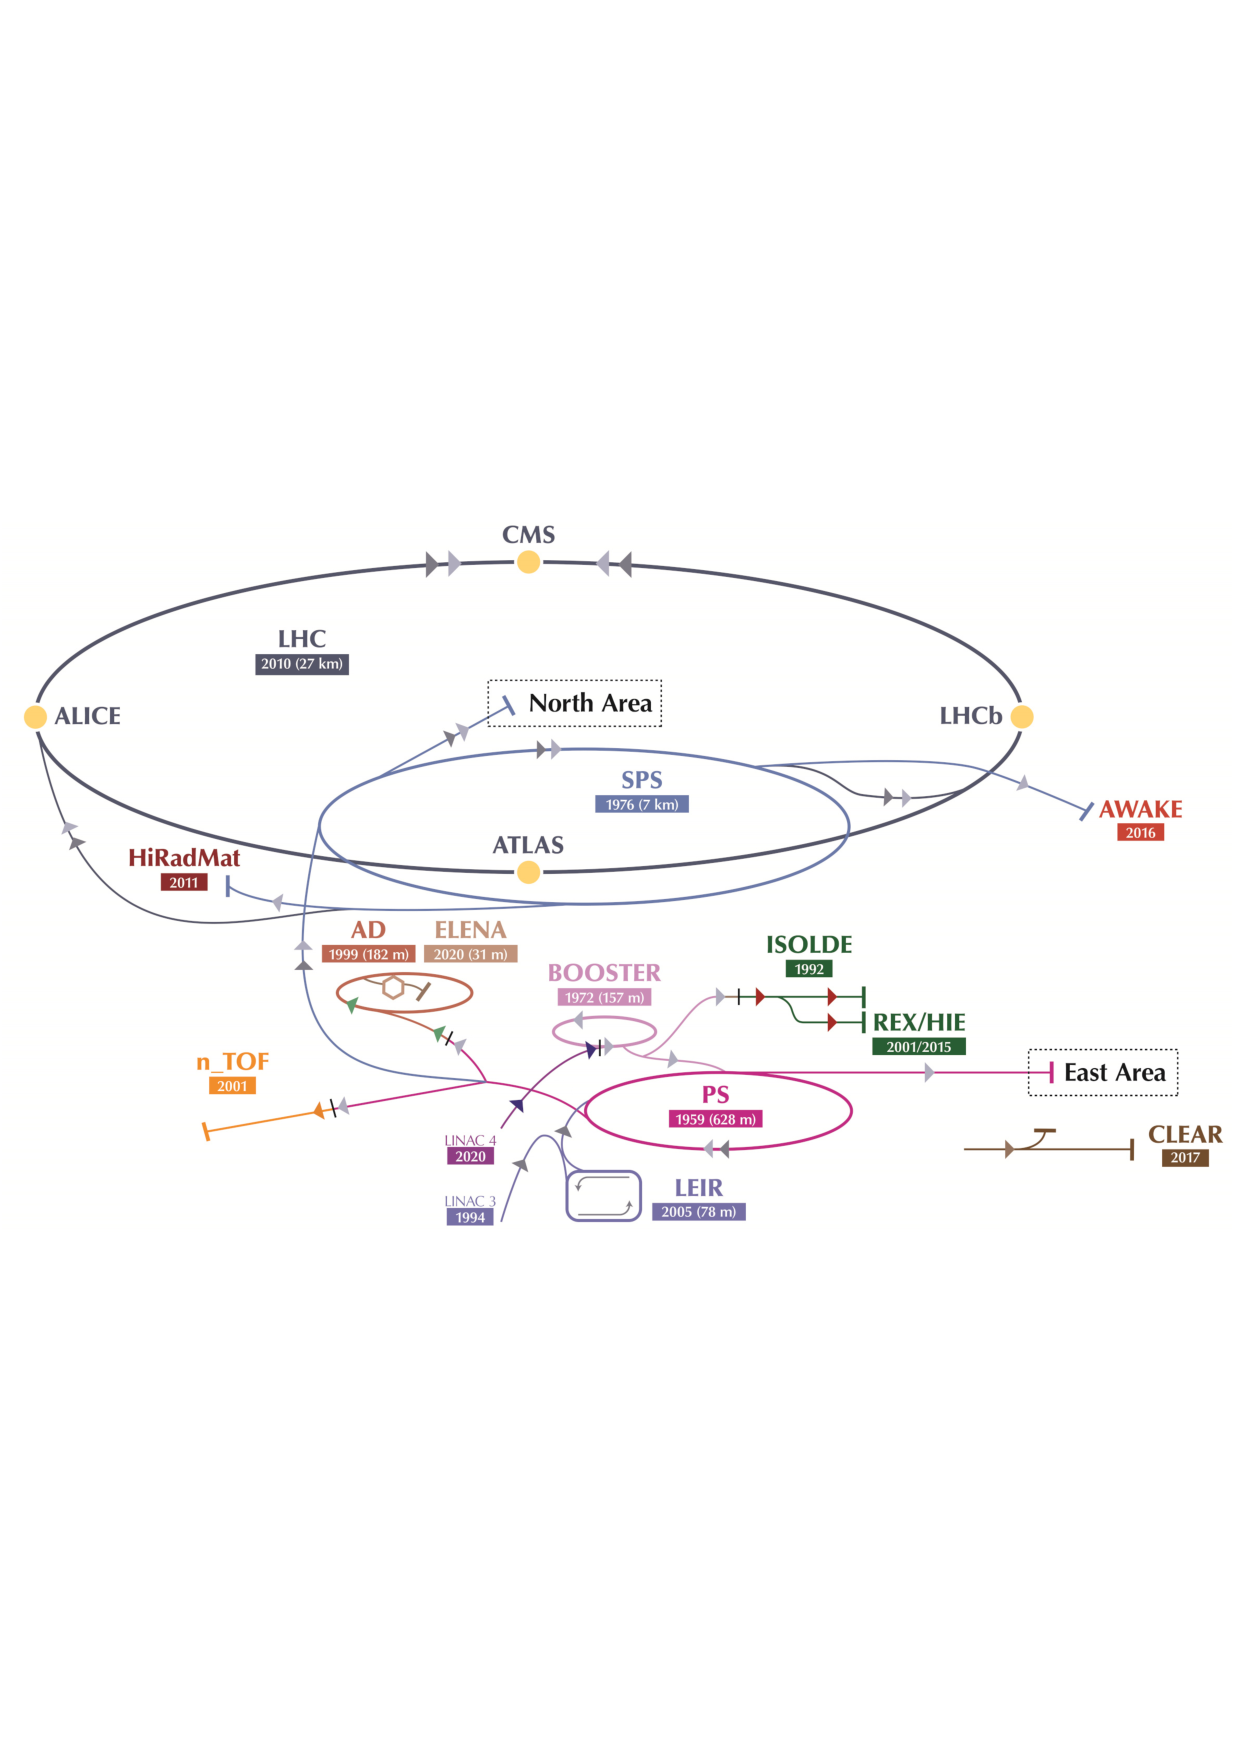
\includegraphics[width=0.8\textwidth]{img/jpeg/lhclhc.pdf}
        \caption[LHC 加速器の全体像]{LHC~加速器の全体像~\cite{URL:01}。LHC~並びに~LHC~の前段加速器の詳細を示している。LHC~には、ATLAS,~ALICE,~CMS,~LHCb~の~4~つの検出器が設置されている。}\label{fig:lhc}
\end{figure}
\section{ATLAS~実験}
ATLAS~実験は~LHC~の衝突点に設置されたATLAS検出器を用いて陽子陽子衝突から~TeV~スケールまでの高エネルギー物理事象の探索を行う実験である。2012~年には、同じ~LHC~の~CMS~実験と共にヒッグス粒子を発見し、標準理論の完成に向けて大きく貢献した~\cite{TR:03,TR:03a}。
本節では、ATLAS~実験の詳細について記していく。
\subsection{ATLAS~検出器}
ATLAS~検出器は、直径~22~m、長さ~44~m~の円筒形で、総重量は~7000~t~という大型汎用検出器である。\figref{fig:atlasdet}にATLAS検出器の全体図を示した。検出器は内側から内部飛跡検出器、電磁カロリメータ、ハドロンカロリメータ、ミューオン検出器という構成になっており、検出器の間には粒子を曲げるための超電導マグネットが設置されている。検出器は広範囲をカバーし、多様な検出器を組み合わせて利用することで高頻度の事象を逃すことなく処理するシステムが構築されている。\figref{fig:disp}は、衝突点より生成された粒子の各検出器における反応の様子を示したイベントディスプレイである。それぞれの検出器の特性をもとに各検出器で様々な粒子の識別を行う。

\begin{figure}[tbp]
    \centering   
    \includegraphics[width=0.9\textwidth,page=1]{img/pdf/ATLAS.pdf}
    \caption[ATLAS 検出器の全体図]{ATLAS 検出器の全体図~\cite{TR:01}。直径~25~m,~長さ~44~m,~重さ~7000~t~の大型汎用検出器。}\label{fig:atlasdet}
\end{figure}

\begin{figure}[htbp]
    \centering   
    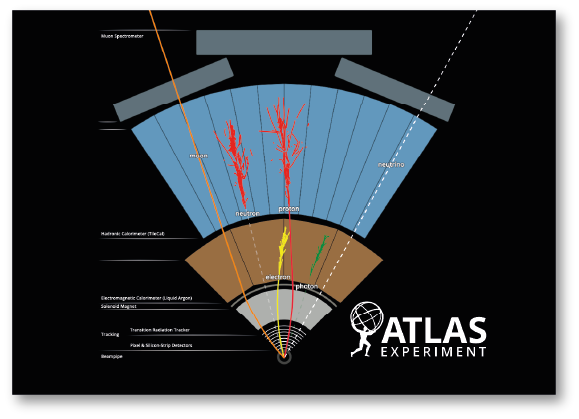
\includegraphics[width=0.85\textwidth]{img/jpeg/how.png}
    \caption[ATLAS~検出器の断面図と通過する粒子のふるまい]{ATLAS~検出器の断面図と通過する粒子のふるまい~\cite{URL:02}。電磁カロリメータでは電子や光子、ハドロンカロリメータでは陽子や中性子、ミューオン検出器ではミューオンの検出を行う。}
    \label{fig:disp}
\end{figure}

\subsection{ATLAS~座標系}
ATLAS~で一般的に利用されている座標系について説明する。\figref{fig:cood}にATLAS検出器のビーム衝突点を原点とした座標系を示した。直交座標系では検出器中心を原点にとり、ビーム軸方向を$z$軸、地面から垂直上方向を$y$軸、LHC~リングの中心を正方向を$x$軸として定義する。またATLAS~では検出器が円筒形のため極座標系が用いられることが多い。任意の$z$座標における動径方向を$R$、方位角方向を$\phi$、極角方向を$\theta$で表す。
$\theta$方向を表す際には擬ラピディティ$\eta$というパラメータ、\equref{eq:eta}がよく用いられる。
擬ラピディティは、ローレンツ変換において不変であるため素粒子実験ではしばしば利用されるパラメータである。
擬ラピディティにより領域を区分することができ、ミューオン検出器においては円筒型の側面部にあたる
$|\eta| < 1.05$をバレル領域、円筒型の底面部にあたる$|\eta| > 1.05$をエンドキャップ領域としている。
また、$\eta>0$の領域を~A-Side、$\eta<0$の領域を~C-Side~と呼んでいる。

\begin{align}
    \eta = -\rm{ln}\left(\rm{tan}\frac{\theta}{2}\right) \label{eq:eta}
\end{align}

粒子のエネルギーや運動量を表す際には、ビーム軸に垂直な成分である横方向エネルギー~($E_{\rm{T}}$)、横方向運動量~($p_{\rm{T}}$)~を利用する。陽子陽子衝突実験において、衝突するクォークやグルーオンの$z$軸方向のエネルギー・運動量には陽子内のパートン分布により不定のため保存則を用いることはできない。一方で、ビーム軸に垂直な方向にはエネルギーおよび運動量の保存則が成立する。従って$E_{\rm{T}}$や$p_{\rm{T}}$は解析において利用されることが多い。またビーム軸に垂直な方向成分の保存則を用いると、ニュートリノ等のATLAS検出器で観測できなかった粒子によるエネルギーの~2~次元のベクトル和を得ることができる。この見えないエネルギーの和を消失横方向エネルギー~(MET)~と呼ぶ。

\begin{figure}[tbp]
    \centering  
    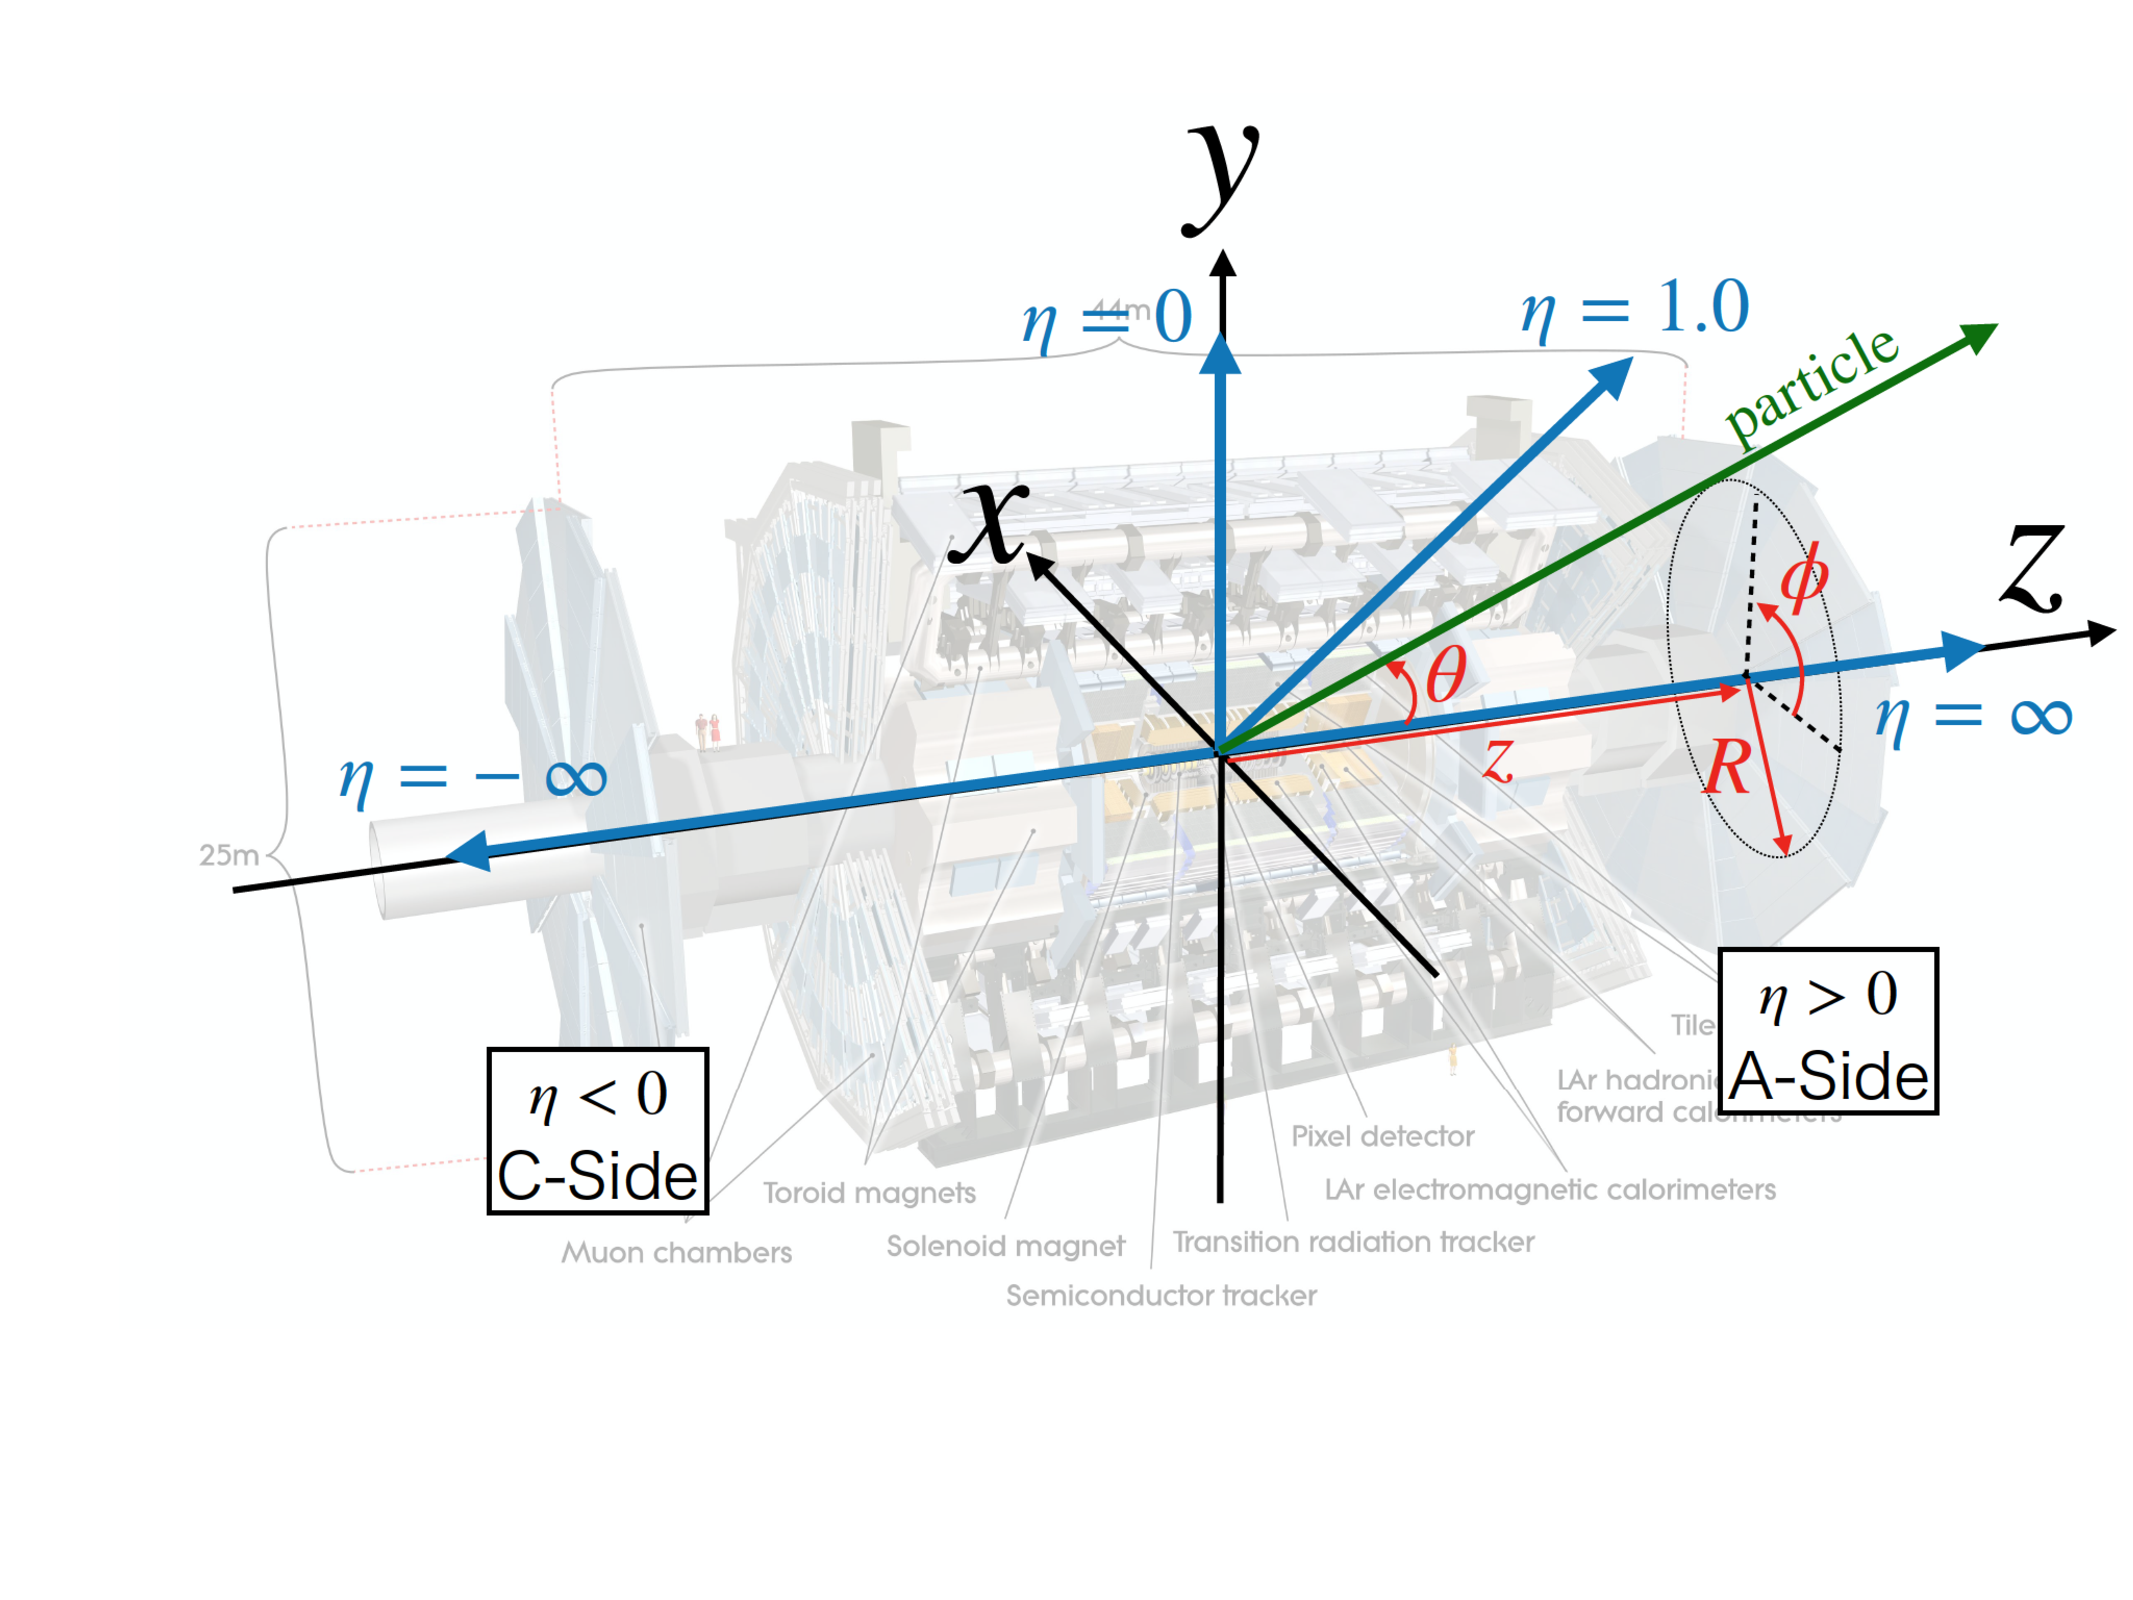
\includegraphics[width=\textwidth,page=1]{img/pdf/cood.pdf}
    \caption[ATLAS~実験において使用される座標系]{ATLAS~実験において使用される座標系。$x,~y,~z$方向に設定される直交座標系と$R,~\phi,~\theta$で定義される極座標系がある。$\theta$方向を表す量として、擬ラピディティ$\eta$が利用される。$\eta>0$を~A-Side、$\eta<0$を~C-Side~と呼ぶ。}\label{fig:cood}
\end{figure}

\subsection{超伝導マグネット}
ATLAS~におけるマグネットシステムは~3~種類の巨大な超電導磁石により構成されている。\figref{fig:mag}にATLAS検出器における超伝導マグネットの構成を示す。一つは中央のソレノイド磁石であり内部検出器の運動量測定に用いられる。流れる電流は~7.73~kA~で、ピーク磁場は~2.6~T~である。その周りを囲むバレル領域のトロイド磁石は、八回対称のリングで構成されており、円周方向の磁場を生成する。流れる電流は~20.5~kA~で、ピーク磁場は~3.9~T~である。エンドキャップ領域のトロイド磁石も同様に円周方向の磁場を生成する。流れる電流は~20.5~kA~で、ピーク磁場は約~4.1~T~である。これらのトロイド磁石はミューオンの運動量を測定するために利用されている。

\figref{fig:mag}に示すように、トロイド磁場の強さは一様ではなく基本的にコイルの配置と同様に八回対称になる。$0<|\eta|<1.4$における磁場の強さは約$1.5\sim5.5~\rm{Tm}$、$1.6<|\eta|<2.7$における磁場の強さは約$1\sim7.5~\rm{Tm}$となる。
磁場の弱い領域においては低い横運動量を持つミューオンと高い横運動量を持つミューオンの曲率の差がなくなり正確な横運動量測定ができなくなる。したがって初段ミューオントリガーにおいては、磁場の弱い領域で正しく運動量判定ができなかった事象を取り除くアルゴリズムが実装されている~(RoI~Mask)。
\begin{figure}[tbp]
        \begin{minipage}{0.49\hsize}
        \centering   
        \includegraphics[width=0.75\textwidth,page=5]{img/pdf/ATLAS.pdf}
        \subcaption{}
        \end{minipage}
        \begin{minipage}{0.49\hsize}
	    \centering
	    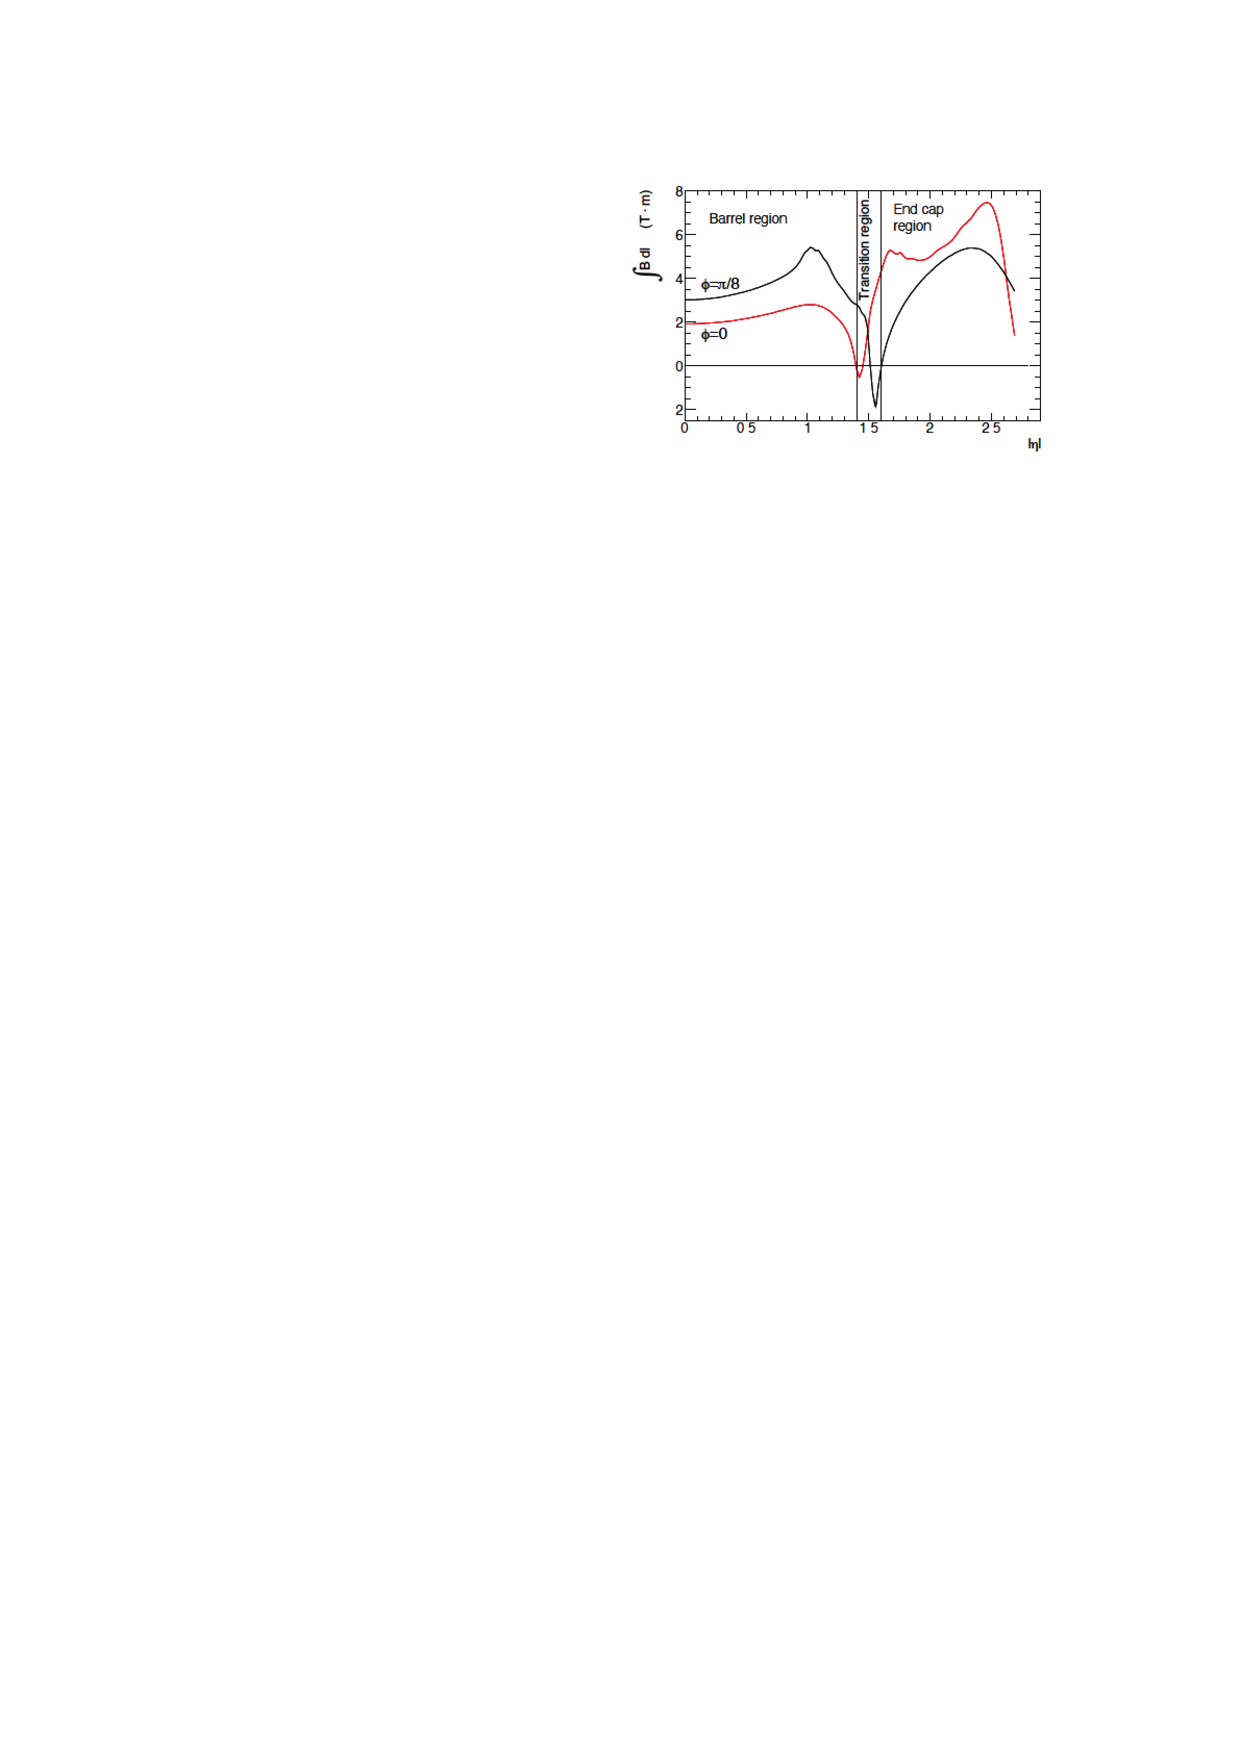
\includegraphics[width=\textwidth,page=1]{img/pdf/mag.pdf}
	    \subcaption{}
	    \end{minipage}
        \caption[ATLAS~検出器における超伝導磁石の構成とトロイド磁石による磁場の分布]{(a)ATLAS検出器における超伝導磁石の構成~\cite{TR:01}。衝突点付近のソレノイド磁石と外側のトロイド磁石で構成されている。トロイド磁場はエンドキャップ領域、バレル領域それぞれにおいて八回対称になるように設定されている。(b)~トロイド磁石による磁場の分布~\cite{TR:01}。無限運動量ミューオンに対するトロイダル磁石の予想磁場積分値を$|\eta|$の関数として表している。}\label{fig:mag}
\end{figure}

\subsection{内部飛跡検出器}
内部飛跡検出器~\cite{URL:19}はビーム衝突点に最も近い位置に設置され、ソレノイド磁石の内部に位置している。内側から順に、ピクセル検出器~(Pixel)、シリコントラッカー~(SCT)、遷移輻射トラッカー~(TRT)~の~3~つで構成されている。
~Pixel~は、最内層にある半導体検出器であり、高い位置分解能を持つ。SCT~はマイクロストリップと呼ばれる細長い有感領域をシリコン上に施した半導体検出器である。そして~TRT~は半径~4~mm~のチューブ型検出器であり、トラッキングのほかに遷移輻射を利用した電子の同定も行っている。
以上の内部飛跡検出器は、いずれもビーム衝突点に近く非常に厳しい放射線環境下にさらされるため、高い放射線耐性が必要不可欠である。\figref{fig:innr}に内部飛跡検出器の概略を示す。

\begin{figure}[tbp]
    \centering   
    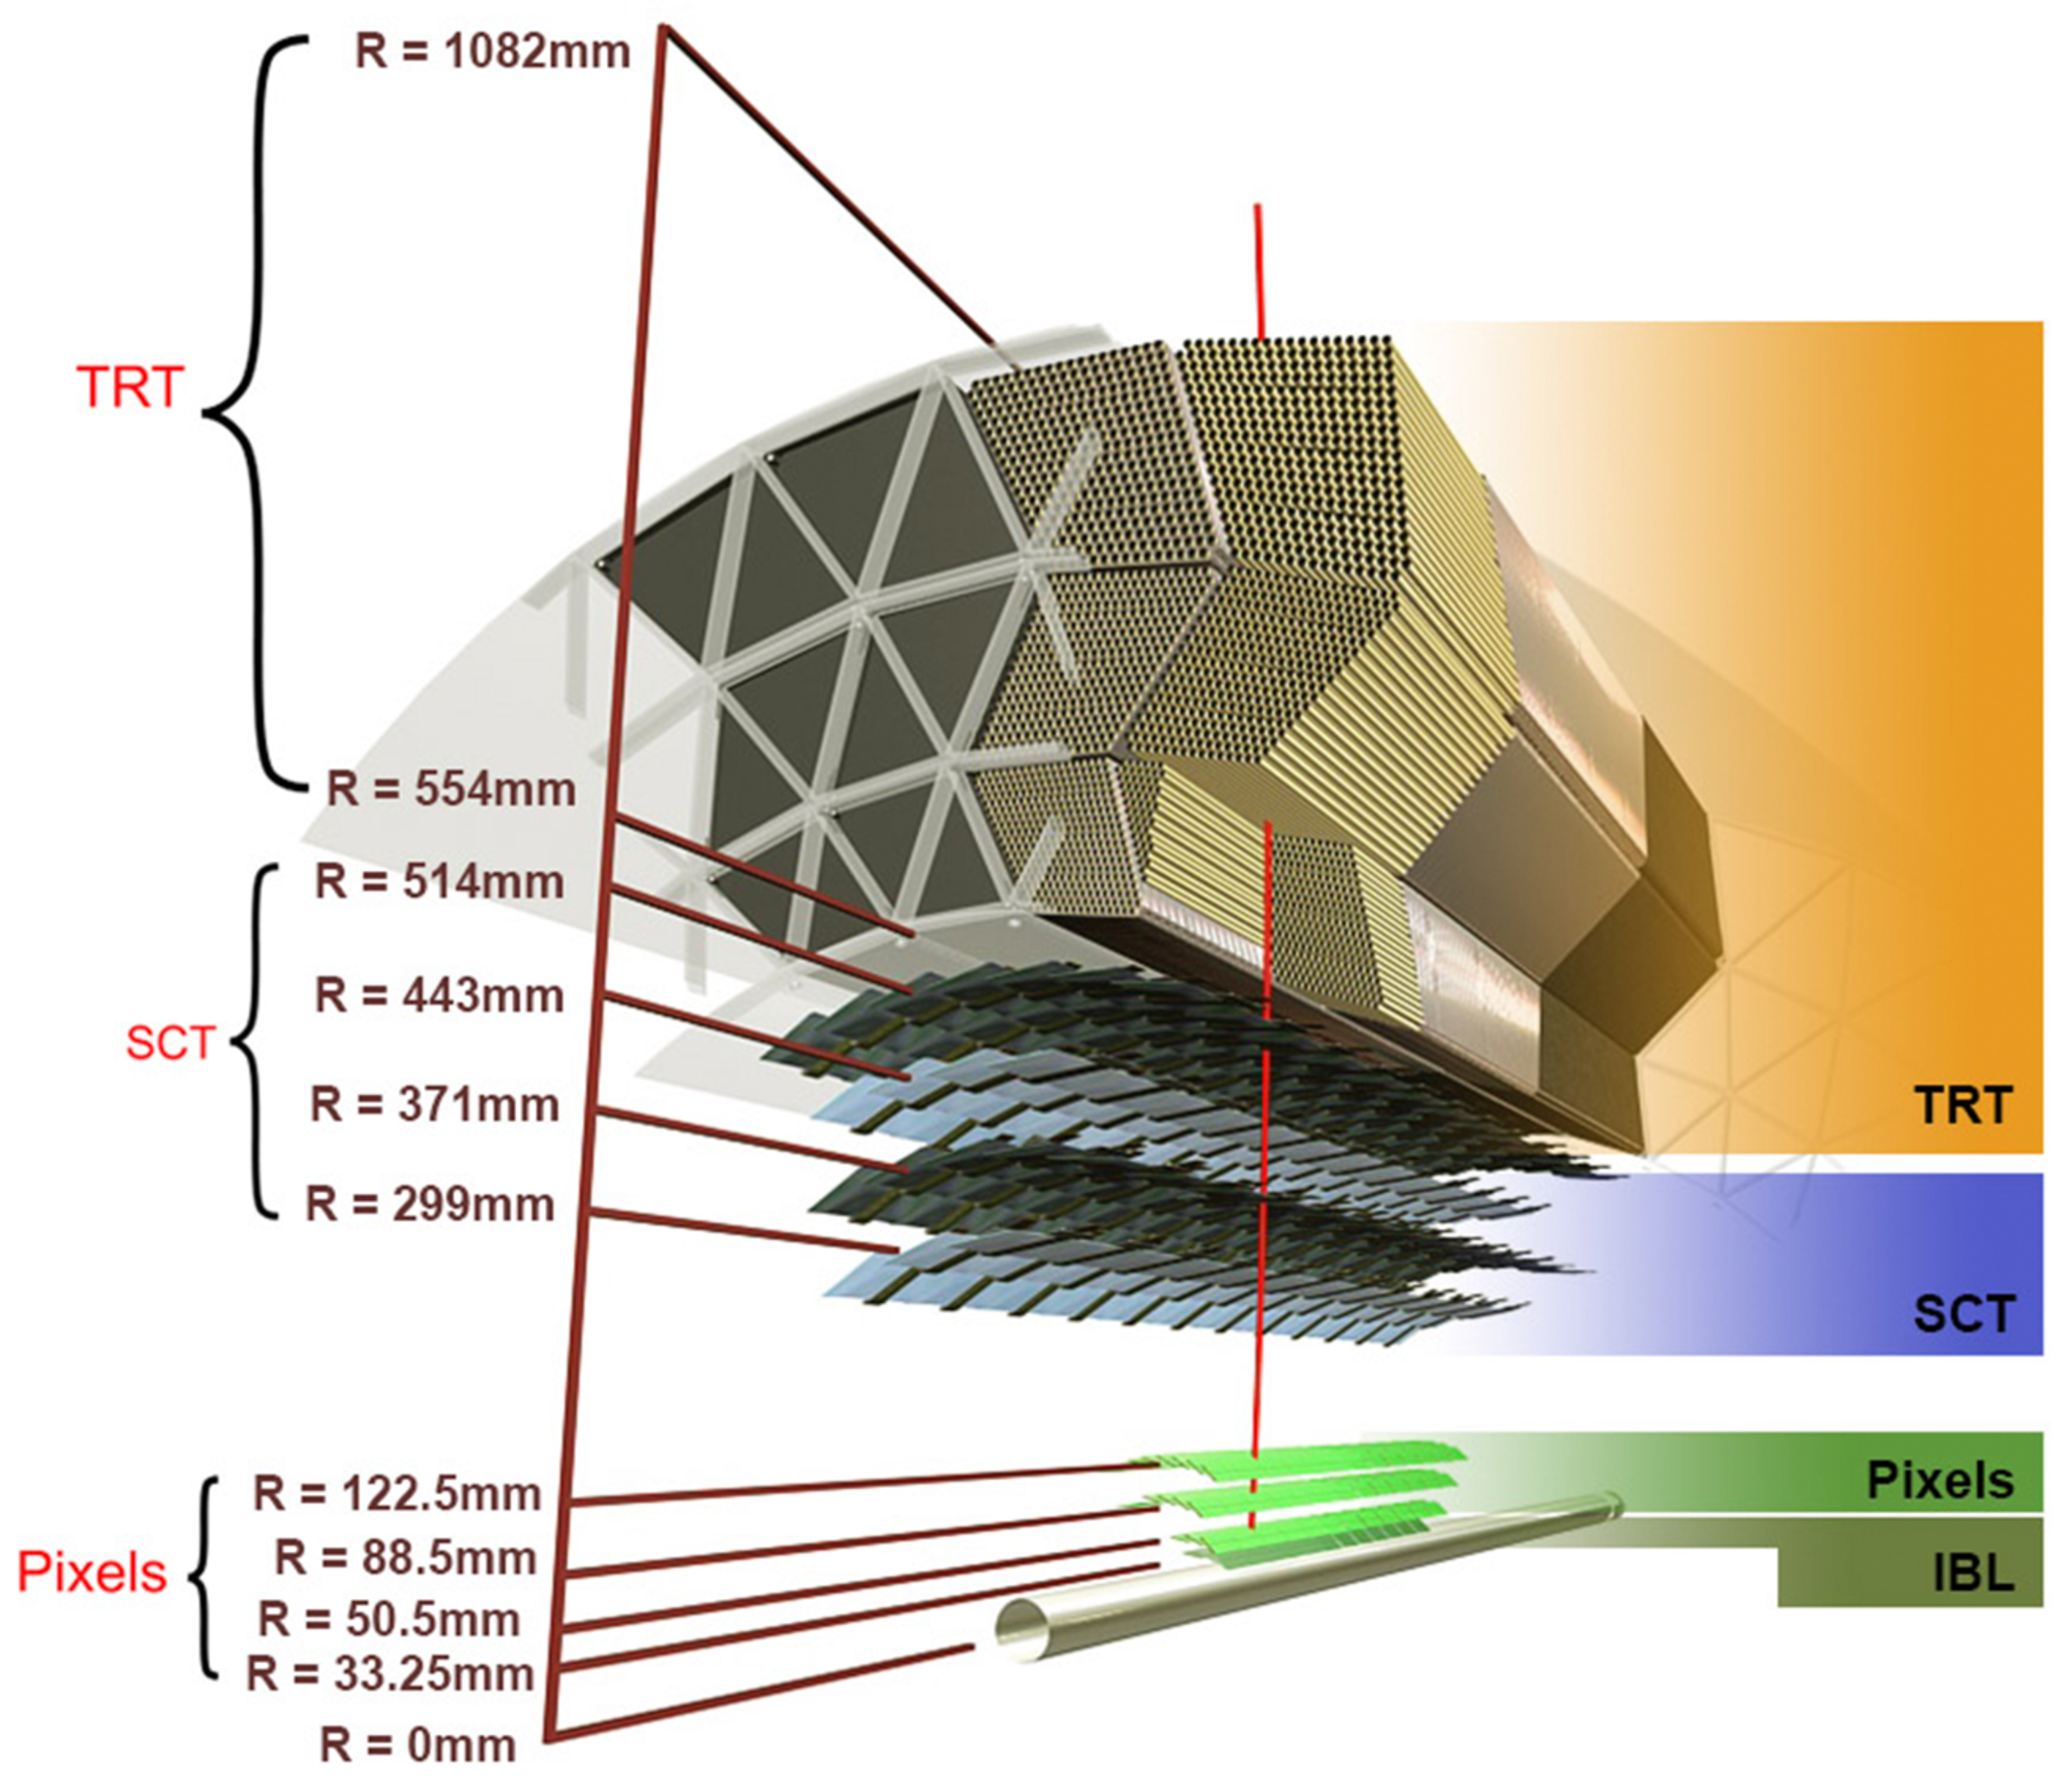
\includegraphics[width=0.8\textwidth,page=1]{img/jpeg/id.pdf}
    \caption[ATLAS~検出器における内部飛跡検出器の構成]{ATLAS~検出器における内部飛跡検出器の構成~\cite{URL:19}。内側から順に~Pixel,~SCT,~TRT~検出器が設置されている。}\label{fig:innr}
\end{figure}

\subsection{カロリメータ}
カロリメータの主な役割は、電子やガンマ線、ジェット等のエネルギーおよび角度の測定である。ATLAS~実験に使用される~4~種類のカロリメータは、電磁カロリメータとハドロンカロリメータの~2~つのいずれかに区分され、広範囲をカバーしている。\figref{fig:calo}にカロリメータの構成を示す。
以下では、それぞれのカロリメータについて簡単に説明する。

\begin{figure}[tbp]
        \centering   
        \includegraphics[width=0.8\textwidth,page=3]{img/pdf/ATLAS.pdf}
        \caption[ATLAS~検出器におけるカロリメータの構成]{ATLAS~検出器におけるカロリメータの構成~\cite{TR:01}。電磁カロリメータは、バレル領域およびエンドキャップ領域の~2~種類。ハドロンカロリメータは、バレル領域のタイル、エンドキャップ領域、フォワード領域の液体アルゴンカロリメータの~3~種類。}\label{fig:calo}
\end{figure}

\subsubsection{電磁カロリメータ}
電磁カロリメータは、アコーディオン構造のからなる鉛の吸収体と液体アルゴンで構成される。放射線耐性に優れており、電子と光子の同定に使用されている。ソレノイド磁石の外側に設置され、バレル領域$\cdot$エンドキャップ領域それぞれをカバーしている。

\subsubsection{ハドロンカロリメータ}
バレル領域では、鉄の吸収体とタイル状のシンチレータから構成されたタイルカロリメータが用いられている。放射線強度がより高いエンドキャップ領域では、銅の吸収体と液体アルゴンから構成されたカロリメータが使用されている。またさらに放射線強度の高いフォワード領域には、銅とタングステンの吸収体と液体アルゴンからなるカロリメータが設置されている。
以上のハドロンカロリメータは、電磁カロリメータの外側に設置されており、ハドロンの同定、エネルギー測定およびジェットの再構成を行う。


\subsection{ミューオン検出器}
終状態に荷電レプトンを含む事象は、ジェットを引き起こすハドロンなどに比べ、飛跡を再構成しやすく、測定装置で捕えやすい。特にミューオンは物質に対する透過力が高く、寿命が長いためにATLAS検出器の外側でもほかの検出器の影響を受けることなく検出することが可能である。ミューオン検出器は、飛跡の精密測定用の~Monitored~Drift~Tube~(MDT)、Cathorde~Strip~Chamber~(CSC)~と、トリガー用の~Resistive~Plate~Chamber~(RPC)、Thin~Gap~Chamber~(TGC)の~4~種類で構成され、ATLAS~検出器の最外層に設置されている検出器である。\figref{fig:mud}に各ミューオン検出器の構成を示す。
\begin{figure}[tbp]
        \centering   
        \includegraphics[width=0.7\textwidth,page=4]{img/pdf/ATLAS.pdf}
        \caption[ATLAS~検出器におけるミューオン検出器の構成]{ATLAS~検出器におけるミューオン検出器の構成~\cite{TR:01}。トリガー用の~RPC,~TGC~と精密測定用の~MDT,~CSC~で構成されている。}\label{fig:mud}
\end{figure}

MDT~はバレル領域とエンドキャップ領域の両方に設置され、直径~30~mm~のドリフトチューブによって構成されている。CSC~はフォワード領域の内側に設置されたストリップチェンバーである。 また~RPC~はバレル領域、TGC~はエンドキャップ領域をカバーするように配置されており、PRC~は~平行平板ガス検出器、TGC~は薄いギャップの~Multi~Wire~Proportional~Chamber~(MWPC)~である。ミューオン検出器の特徴の詳細に関しては、\tbref{tb:muon}に記す。
\begin{table}[tbp]
	\centering
	\begin{tabular}{c|ccc}\hline
	    検出器 & 役割 & カバー領域 & チャンネル数 \\ \hline\hline
		MDT & 運動量測定 & $0<|\eta|<3.0$ & 約370,000 \\ 
		CSC & 運動量測定 & $2.0<|\eta|<3.0$ & 約67,000 \\
        RPC & トリガー & $0<|\eta|<1.05$ & 約350,000 \\
        TGC & トリガー & $1.05<|\eta|<2.04$ & 約320,000 \\ \hline 
	\end{tabular}
	\caption{各ミューオン検出器における役割や特徴の一覧}
    \label{tb:muon}
\end{table}

バレル領域においてミューオン検出器は、大きく分けて円筒型の側面部~3~箇所に配置されている。またエンドキャップ領域では円筒型の底面部~3~箇所に配置されている。バレル・エンドキャップそれぞれにビーム衝突点に近い方から、Inner,~Middle,~Outer~と呼んでいる。\figref{fig:tgc000}にATLAS検出器における断面図と~TGC~検出器の配置を示した。TGC~は、Middle~に~M1,~M2,~M3~の~3~ステーション、トロイドマグネット内側の~Inner~に~EIFI~ステーションの合計~4~ステーションで構成されている。TGC~検出器における構成やエレクトロニクスに関する詳細は\chapref{chap:4}で述べる。
\begin{figure}[tbp]
    \centering
    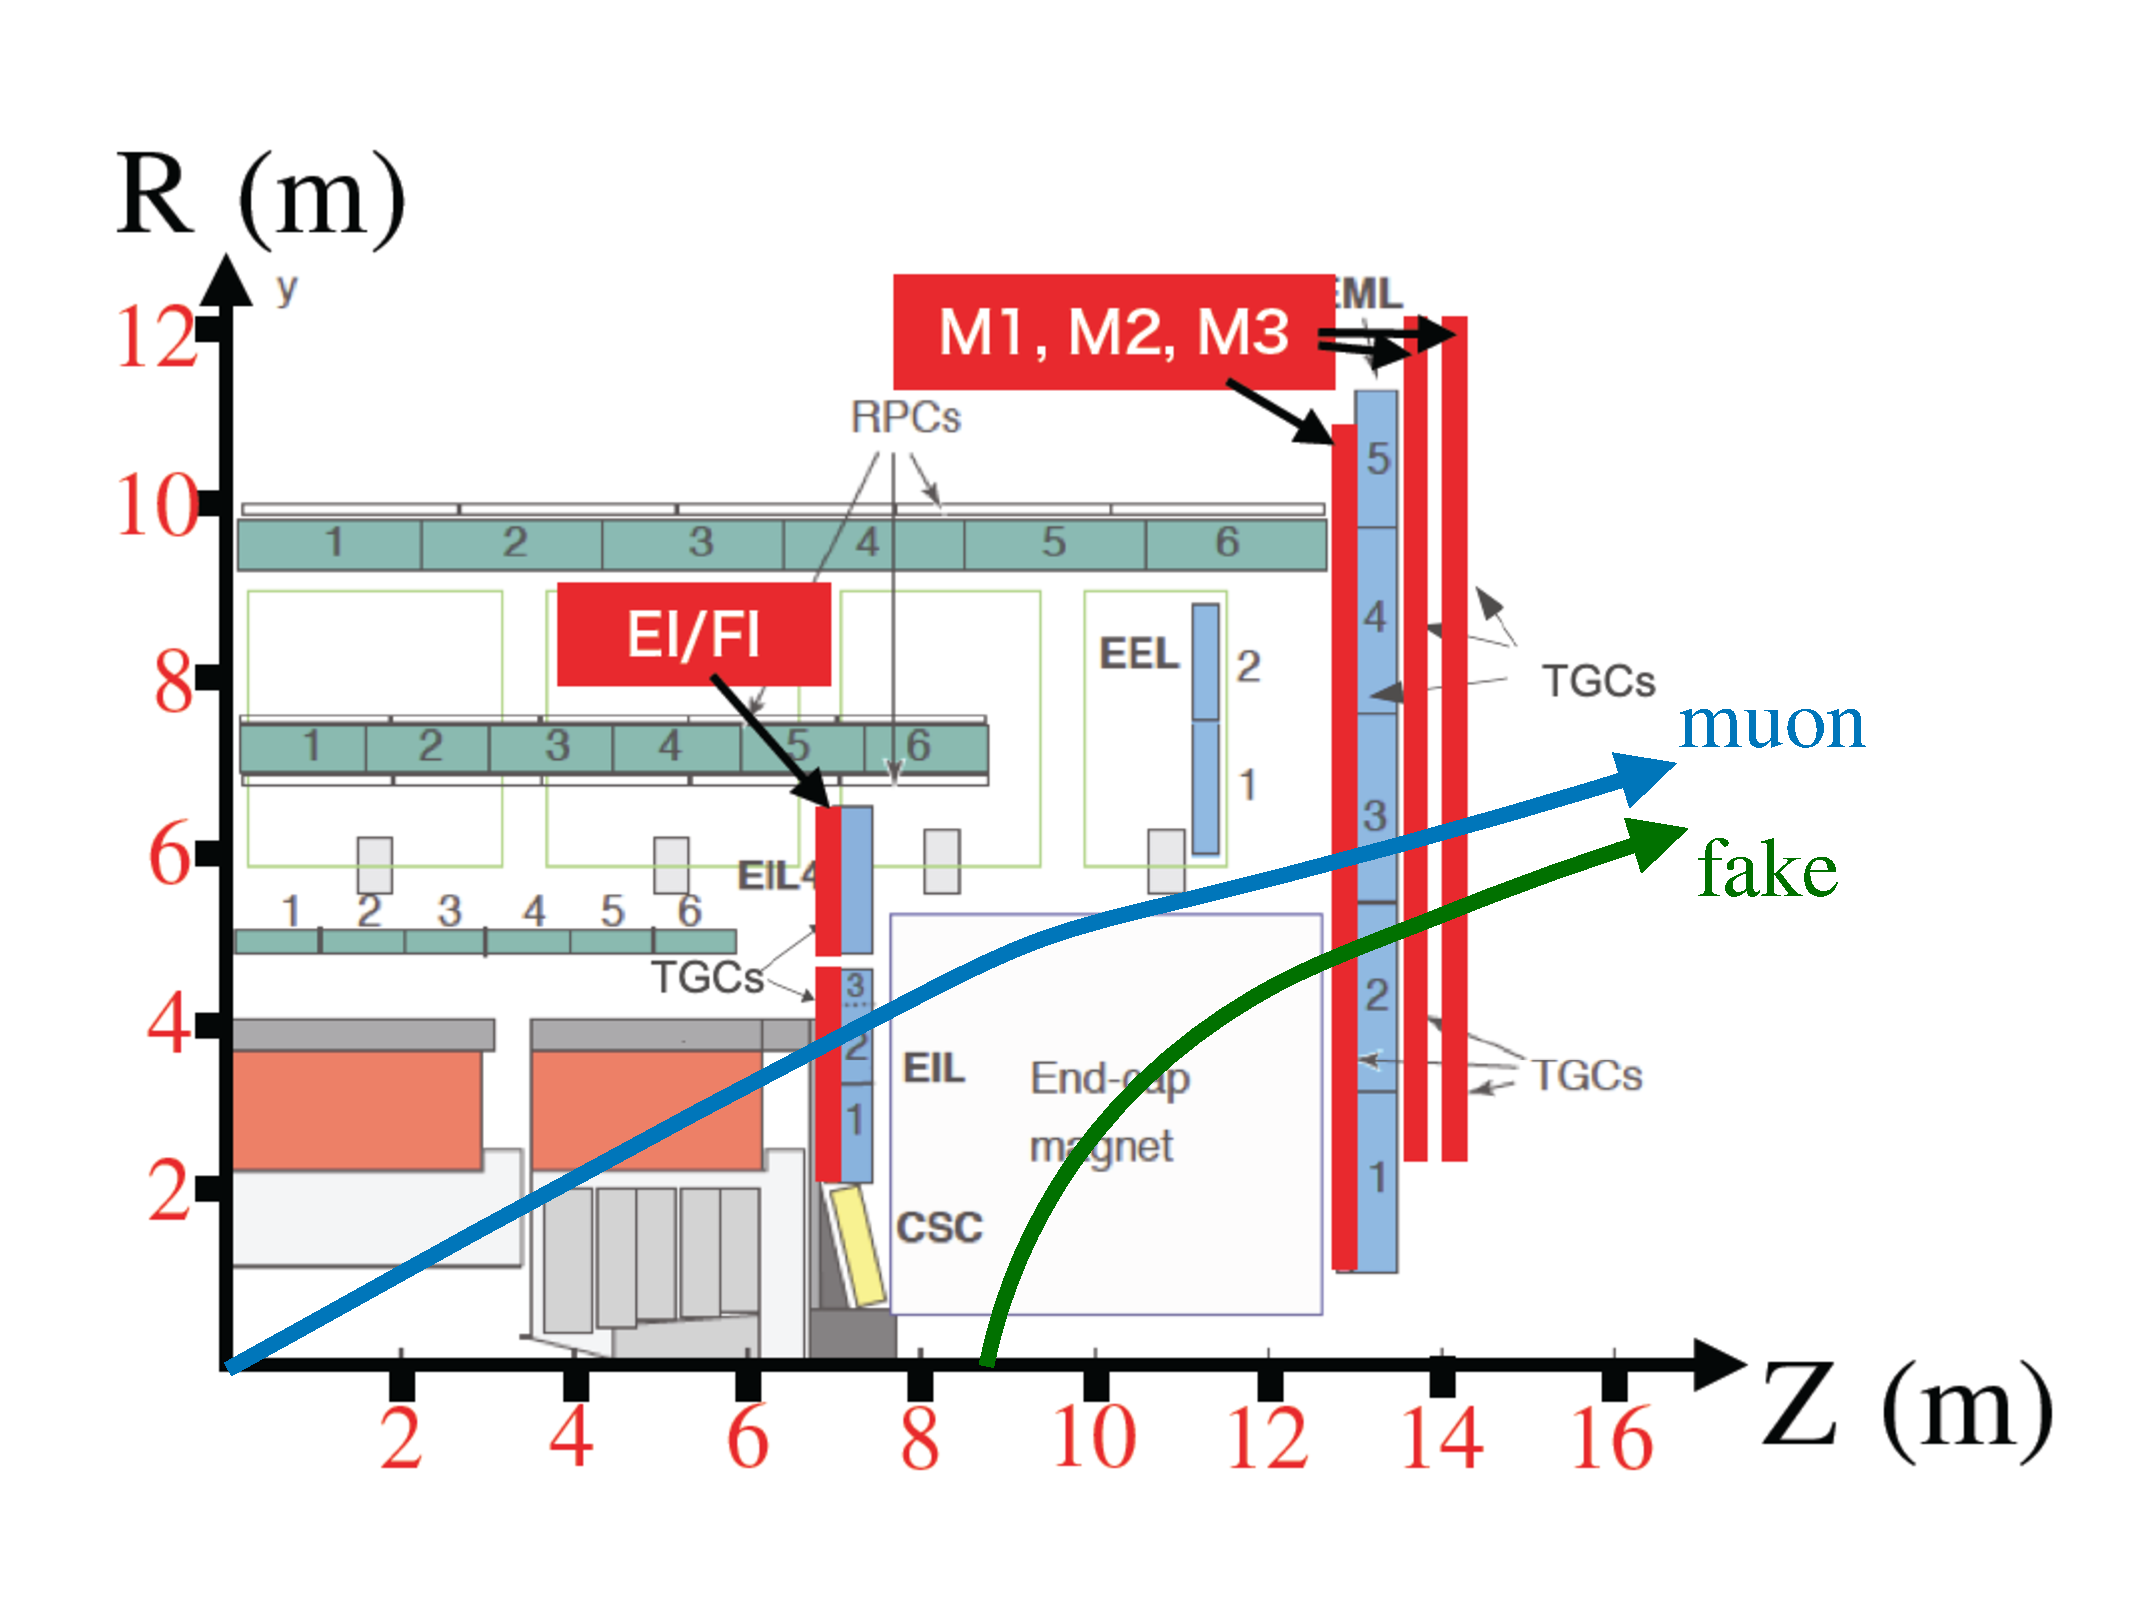
\includegraphics[width=0.8\textwidth,page=1]{img/pdf/fake.pdf}
    \caption[Run~2~におけるATLAS検出器を$R-z$方向から見たときの断面図および~TGC~各ステーションの配置]{Run~2~におけるATLAS検出器を$R-z$方向から見たときの断面図および~TGC~各ステーションの配置~\cite{TR:01}。Big~Wheel~は、M1~(3~層)、M2~(2~層)、M3~(2~層)の計~7~層で構成されており、Small~Wheel~は、EIFI~(2~層)~で構成されている。また青の矢印は衝突点で生成されたミューオンの飛跡、緑の矢印はビームパイプ由来の低速粒子の飛跡を示す。}\label{fig:tgc000}
\end{figure}

超電導トロイダル磁石は、バレル領域およびエンドキャップ領域にそれぞれ$\phi$方向の磁場を生成している。$\phi$方向の磁場によって$R-z$平面内で曲げられたミューオンの曲率を測定することで運動量を決定する。理想的にはミューオンは$R-z$平面内で曲がるが、実際は磁場の大きさが一様でないため$\phi$方向にも曲がる。トリガー用の~2~つの検出器~(RPC,~TGC)~は、$\phi$方向の座標を測る役割も担っている。

\subsubsection{Run~3~におけるミューオン検出器のアップグレード}
初段ミューオンエンドキャップトリガーでは、\figref{fig:tgc000}で示したようなビームパイプから発生した陽子などの低速粒子による影響が課題となっていた。これらの粒子が高い$p_{\rm{T}}$を持つミューオンと同じ角度で入射した場合、誤ってトリガーを発行してしまう。2012~年に取得した~Run~1~の解析結果によると、初段エンドキャップミューオントリガーで出力されたうちの約$90\%$がフェイクであった~\cite{TR:05}。その後の~Run~2~では、エンドキャップトロイドマグネットの内側に設置されたタイルカロリメータおよび~TGC~EIFI~とのコインシデンスを導入した。このようなインナーコインシデンスを要求することで、$1.05<|\eta|<1.7$の領域におけるフェイクトリガーの削減に成功している。

$1.92<|\eta|<2.4$の領域ではインナーコインシデンスを行うための検出器が設置されていないため、フェイクトリガーが多く残っており、$1.05<|\eta|<1.92$の領域においてもフェイク削減の余地は残っている。そこで~Run~3~においてはさらなるフェイクトリガーの削減を目指し、トロイド磁場領域の内側に~New~Small~Wheel~(NSW)~および~RPC~Barrel~Inner~Small~sector~78~(RPC~BIS78)~の~2~つの検出器を新たに導入する。\figref{fig:innercoin}に示すように、Run~3~では~2~つの検出器の導入でさらなるフェイクトリガーの削減が可能であることが見積もられている。Run~3~における~新検出器導入後のATLAS検出器の断面図を\figref{fig:cut3}に示す。
\begin{figure}[tbp]
        \centering   
        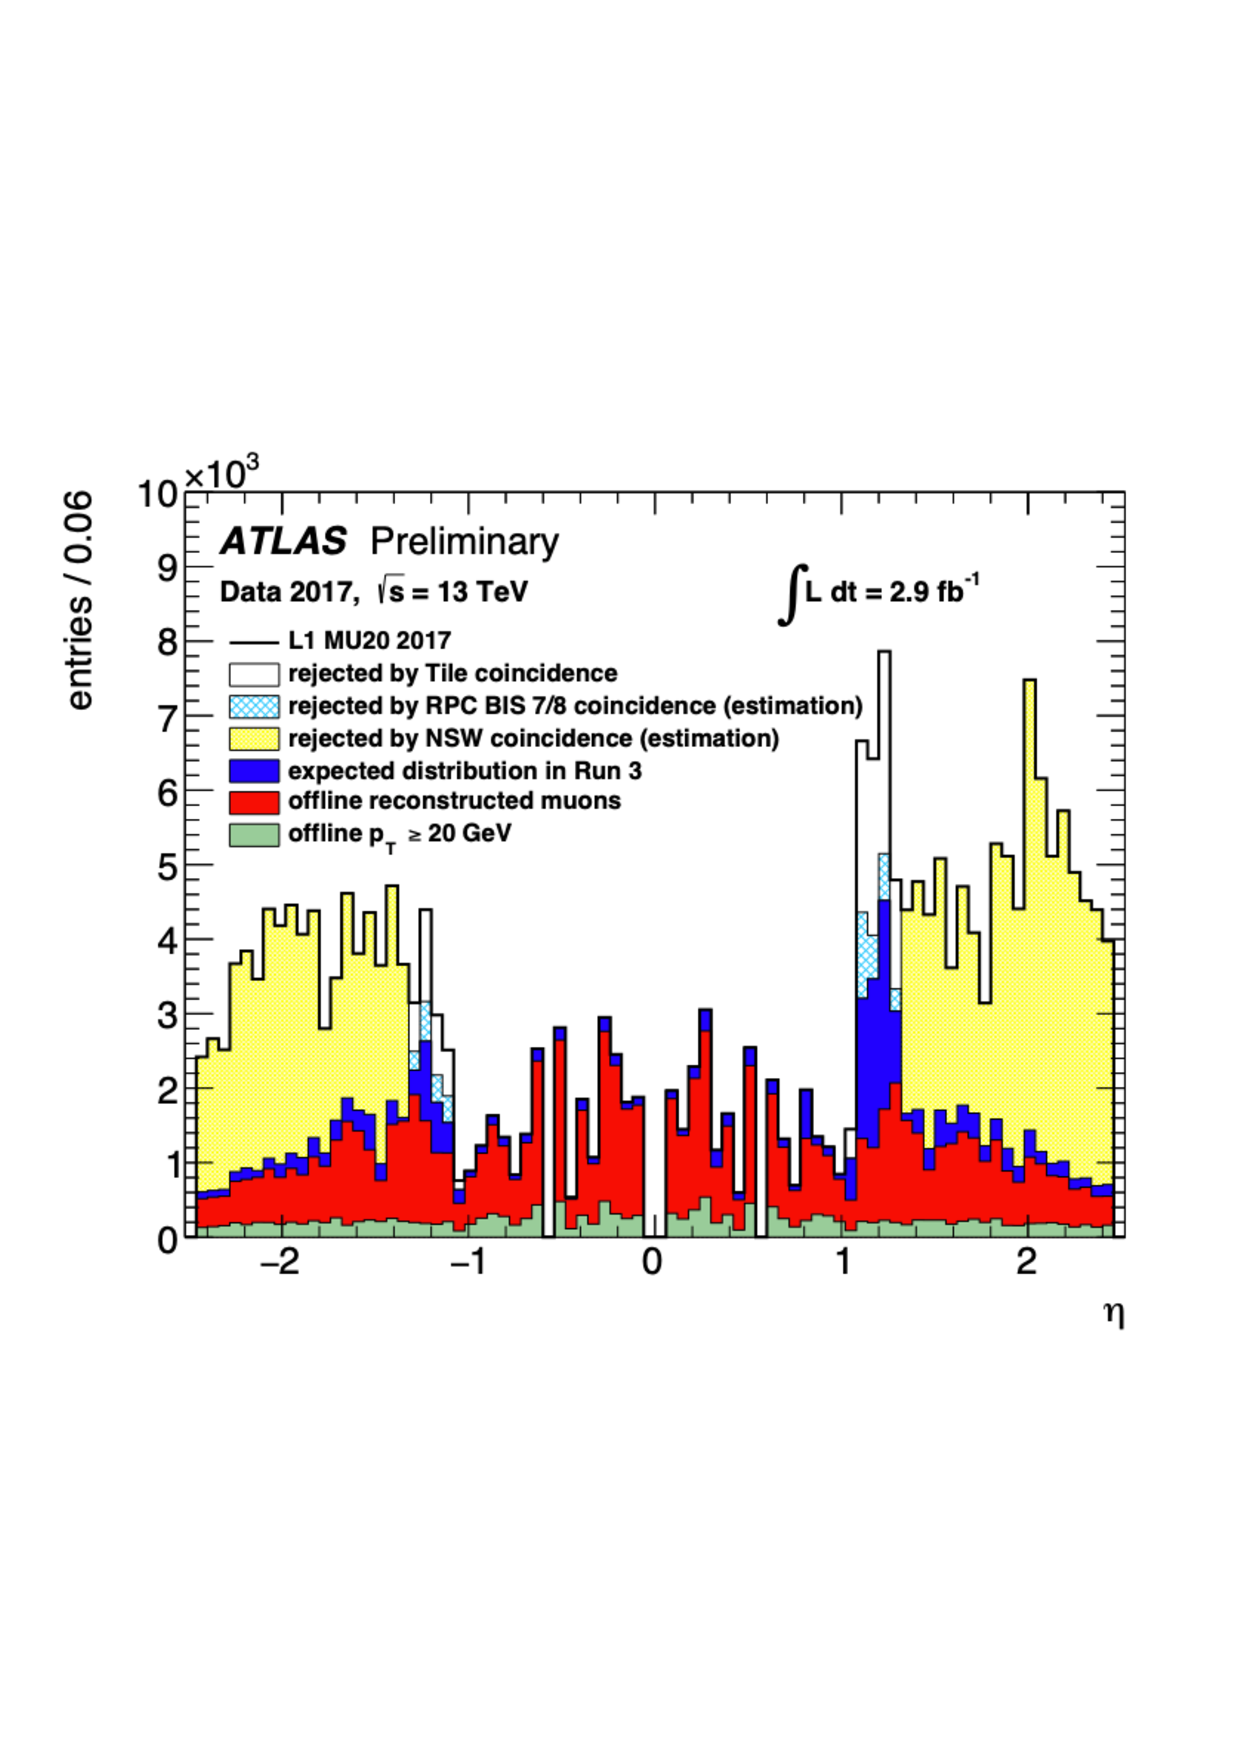
\includegraphics[width=0.7\textwidth,page=1]{img/pdf/inner.pdf}
        \caption[インナーコインシデンスによるフェイクトリガーの削減]{インナーコインシデンスによるフェイクトリガーの削減~\cite{shiomi}。Run~3~における初段ミューオントリガーを用いて選出したミューオン候補数の$\eta$分布の予測。タイル、RPC~BIS78~および~NSW~によって削減できるミューオン候補の数を示している。}
        \label{fig:innercoin}
\end{figure}
\begin{figure}[tbp]
        \centering   
        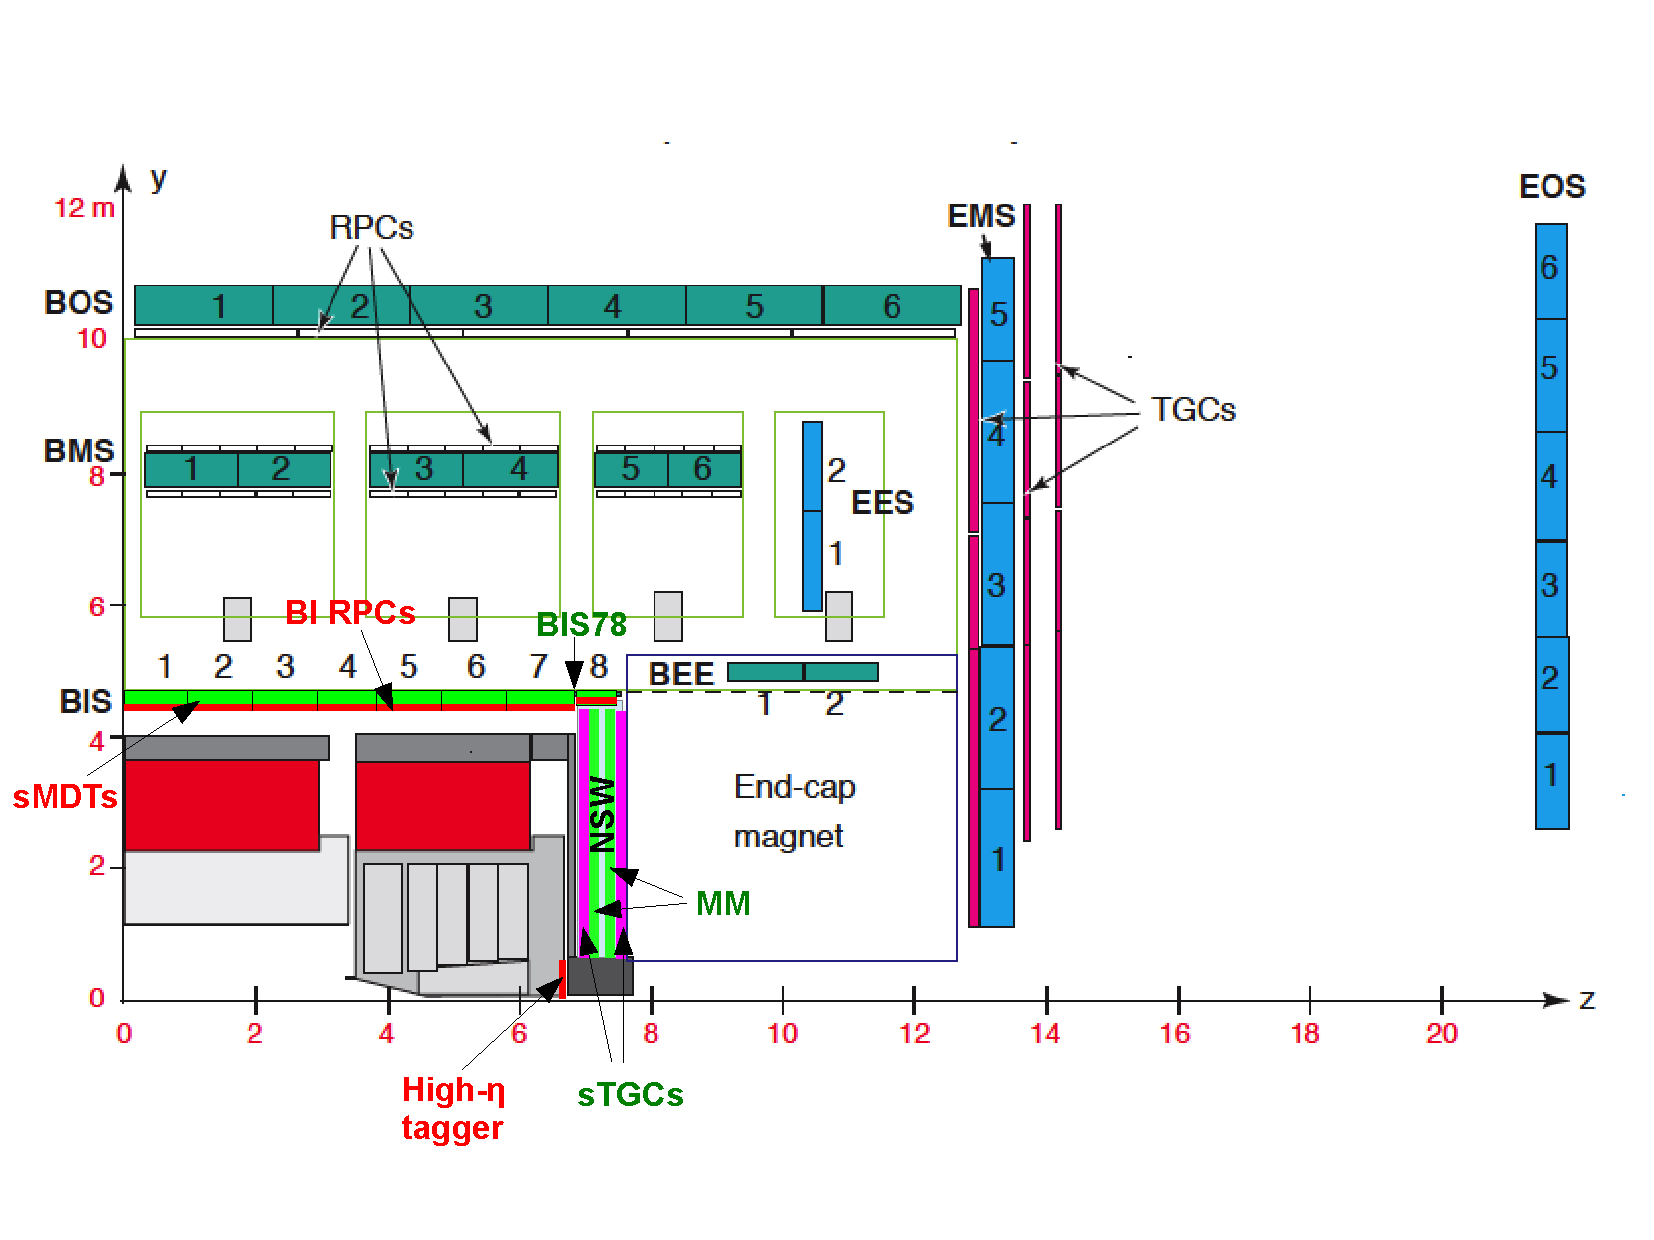
\includegraphics[width=0.8\textwidth,page=1]{img/pdf/ch01_fig_03a.pdf}
        \caption[NSW~および~RPC~BIS78~が導入された~Run~3~におけるATLAS検出器断面図]{NSW~および~RPC~BIS78~が導入された~Run~3~におけるATLAS検出器断面図~\cite{TR:04}。}
        \label{fig:cut3}
\end{figure}
\figref{fig:nsw}に~NSW~の構成を示す。
\begin{figure}[tbp]
    \begin{minipage}{0.49\hsize}
	\centering			
	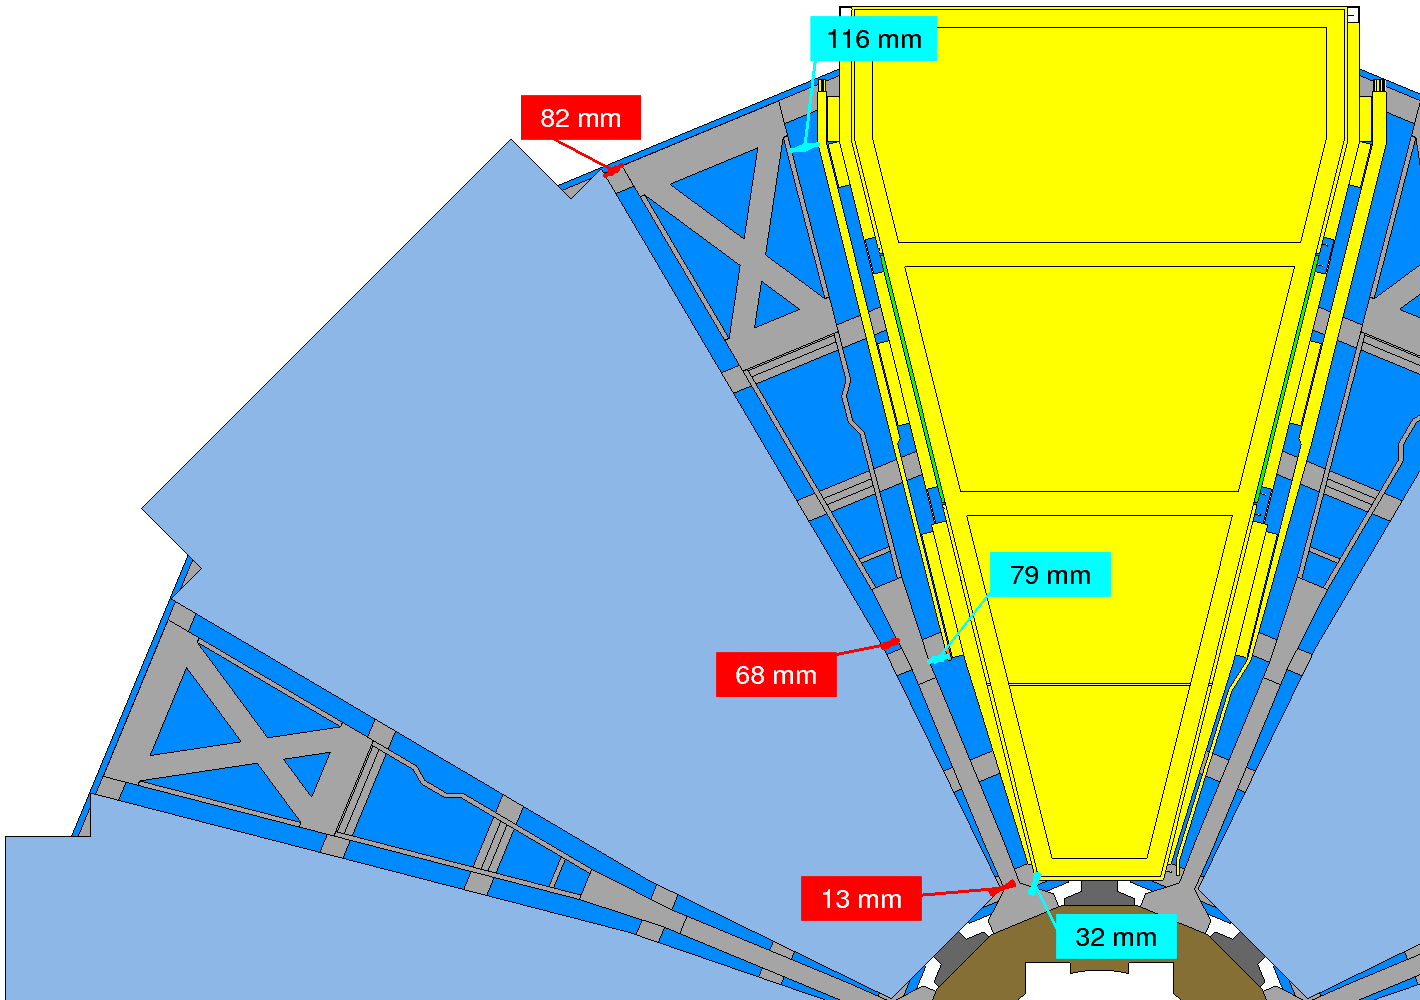
\includegraphics[width=\textwidth,page=1]{img/pdf/fig_026c.png}
	\subcaption{}
	\end{minipage}
	\begin{minipage}{0.49\hsize}
	\centering
	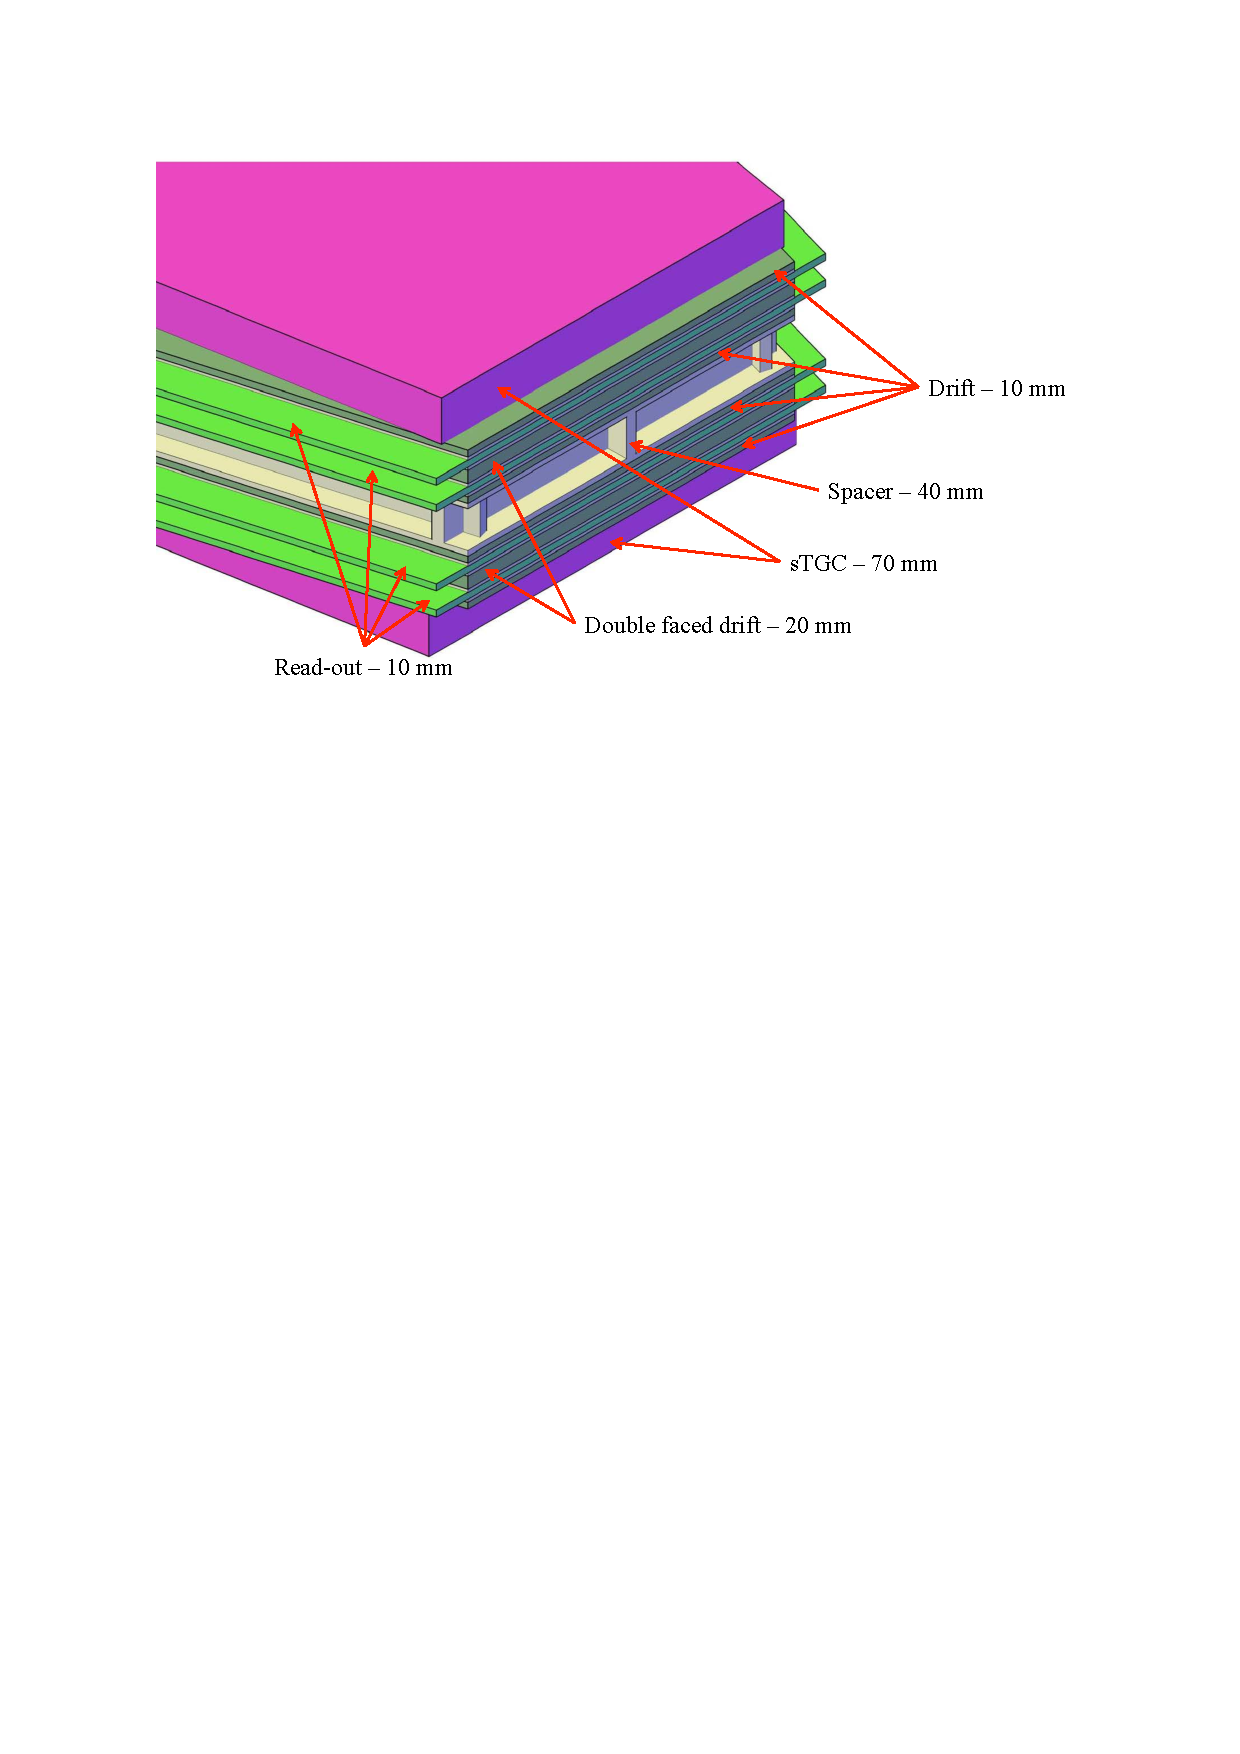
\includegraphics[width=\textwidth,page=1]{img/pdf/fig_042a.pdf}
	\subcaption{}
	\end{minipage}
    \caption[New~Small~Wheel~の構成]{New~Small~Wheel~の構成~\cite{AR:14}。4~層の~sTGC~の間に、4~層の~MM~が~2~台挟まれる構造となっている。(a)~チェンバーの全体図。(b)~NSW~の構成。}
    \label{fig:nsw}
\end{figure}
NSW~は$1.3<|\eta|<2.7$の領域をカバーするガス検出器である。NSW~は、Run~2~で使用されていた~TGC~FI、MDT~EIL~チェンバー、CSC~と入れ替わる形で導入される。したがって、NSW~は~TGC~FI~が担っていたミューオントリガーの役割および~MDT~と~CSC~が担っていた飛跡の精密測定の役割を果たすこととなる。そのため、NSW~は~small-strip~TGC~(sTGC)~と~Micromegas~(MM)~という二つの異なる技術の検出器で構成されている。NSW~を導入することでインナーコインシデンスの領域が$|\eta|<2.4$まで拡張される。

\figref{fig:bis}に~RPC~BIS78~の構成を示す。
\begin{figure}[tbp]
        \centering   
        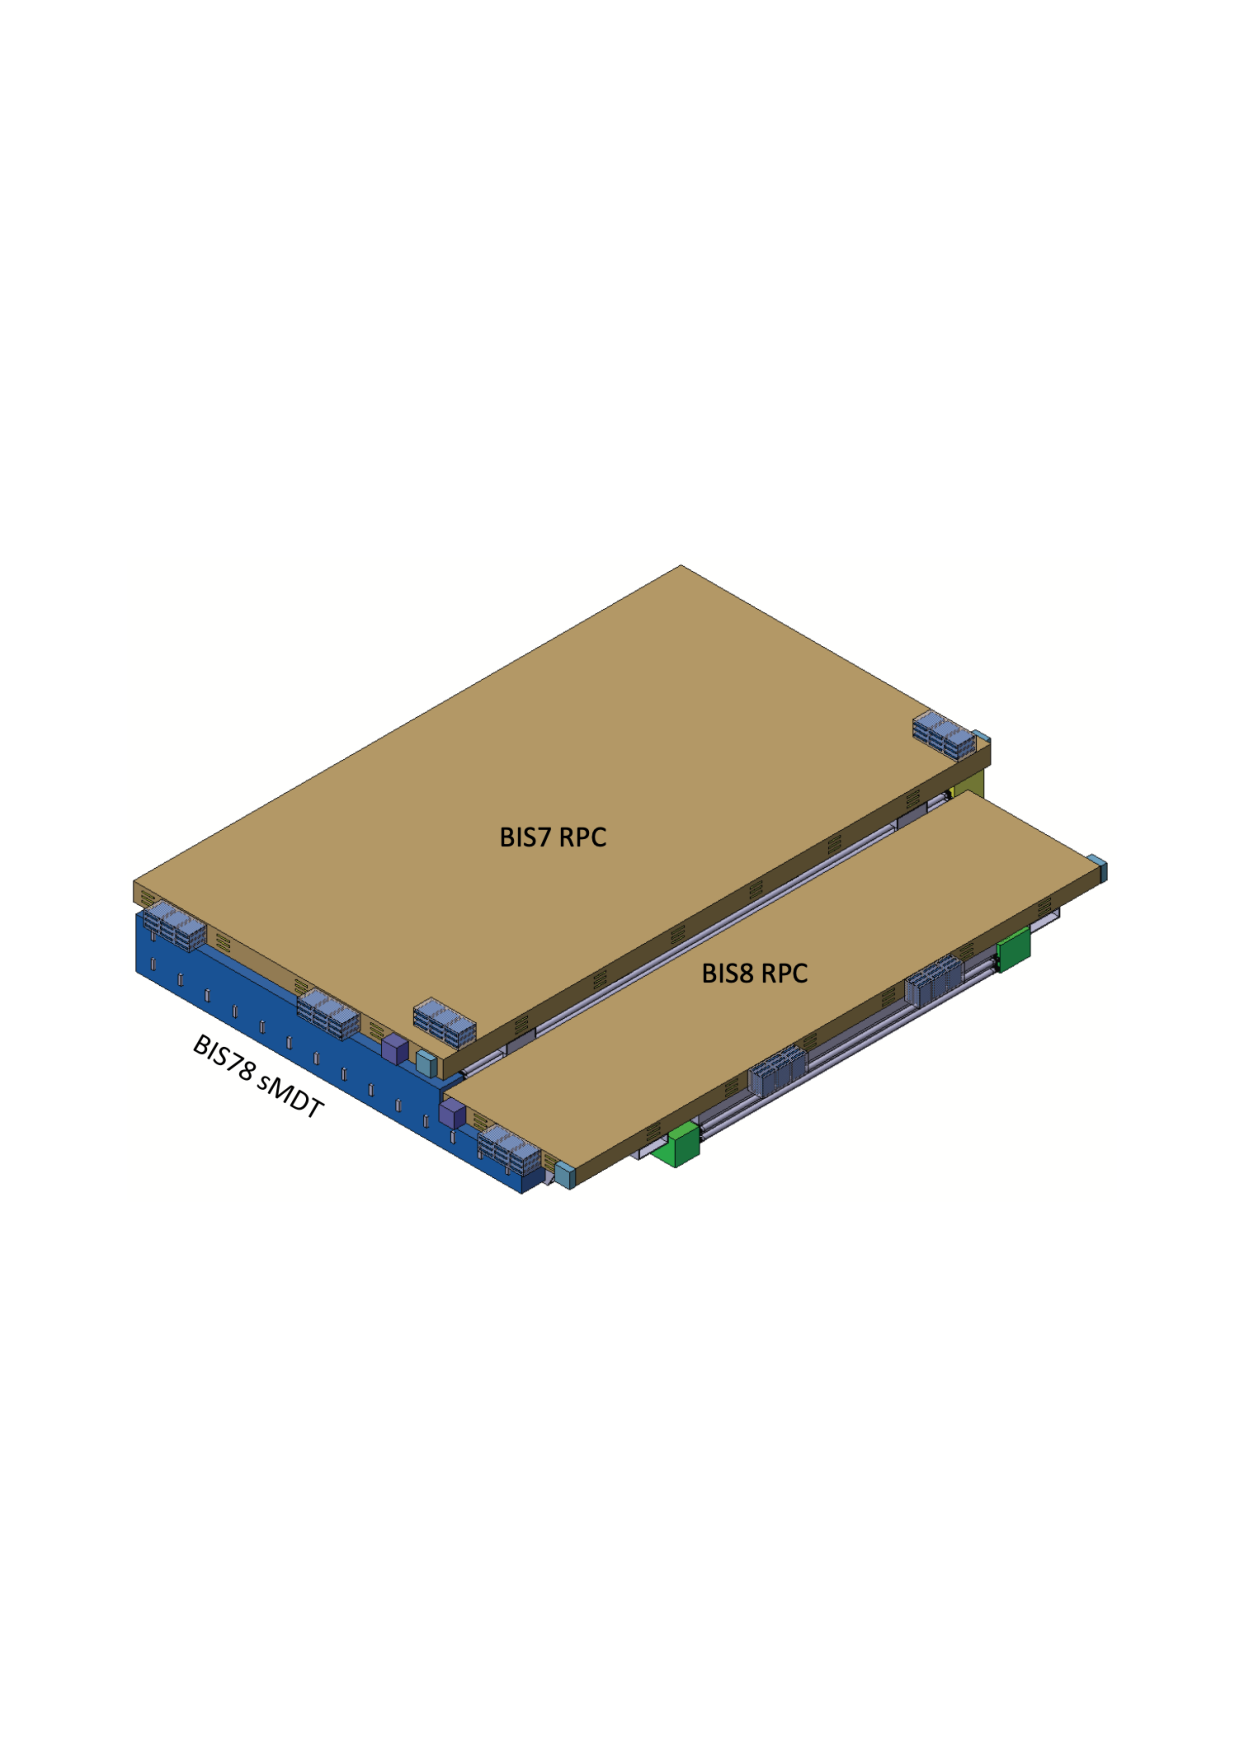
\includegraphics[width=0.8\textwidth,page=1]{img/pdf/bis.pdf}
        \caption[RPC~BIS78~の構成]{BIS78~の構成~\cite{TR:04}。RPC~および~sMDT~で構成される。}
        \label{fig:bis}
\end{figure}
Run~3~ではより高精度な測定を行うために~RPC~および~small-diameter~MDT~(sMDT)~を組み合わせた~RPC~BIS78~を新たに設置する。RPC~BIS78~は$1.0<|\eta|<1.3$の領域をカバーし、3~層のガス層で構成される。ガス層の厚みは約1~mmで、従来の~RPC~の半分になっている。ガス層は従来の~RPC~と同様に~2~次元方向のストリップで$\eta,~\phi$方向が測定できる。

\section{ATLAS~トリガーシステム}\label{sec:ttri}
LHC~での陽子陽子衝突から生成される粒子は~ATLAS~のトリガーシステムを介して選別される。
ATLAS~実験では、陽子がクォークとグルーオンとの複合粒子であることと高いルミノシティであることから、非常に高いイベントレートとなることが考えられる。トリガーシステムにおいては、物理解析のために必要な情報をいかに効率よく正確に選別できるかが鍵を握る。

ATLAS~実験の高頻度~(40~MHz)~陽子バンチ衝突に対して、最終的にデータとしての記録を許容できるイベントレートは数~kHz~である。この制限を満たし効率よくトリガーを行うために、ATLAS~実験ではハードウェアベースの初段トリガー~(Level-1~Trigger:~L1)~とソフトウェアベースの後段トリガー~(High-Level~Trigger:~HLT)~の二段階で実装されている。
\figref{fig:trigger}において、ATLAS 実験におけるトリガーと読み出し処理の流れについて示す。
本節では、ATLAS~実験におけるトリガーシステムについて詳しく説明する。
\begin{figure}[tbp]
        \centering   
            \includegraphics[width=\textwidth,page=2]{img/pdf/tdaq-run3-schematic-withoutFTK.pdf}
        \caption[Run~3~における~ATLAS~トリガーシステムの流れ]{Run~3~における~ATLAS~トリガーシステムの流れ~\cite{URL:07}。L1~では$2.5~\mu\rm{s}$以内にイベントレートを$100~\rm{kHz}$にまで削減する。L1~には~L1Calo,~L1Muon,~L1Topo~の~3~種類が存在する。HLT~ではソフトウェアベースでより詳細にトリガーを行い、数秒以内にイベントレートを数~kHz~にまで削減する。}\label{fig:trigger}
\end{figure}

\subsection{初段トリガー}\label{subsec:l1tri}
\subsubsection{初段トリガーでの処理の流れ}
初段トリガー~(L1)~におけるデータ処理の流れについて説明する。
\figref{fig:pipe}に~L1~における情報処理の流れを示す。
\begin{figure}[tbp]
        \centering   
        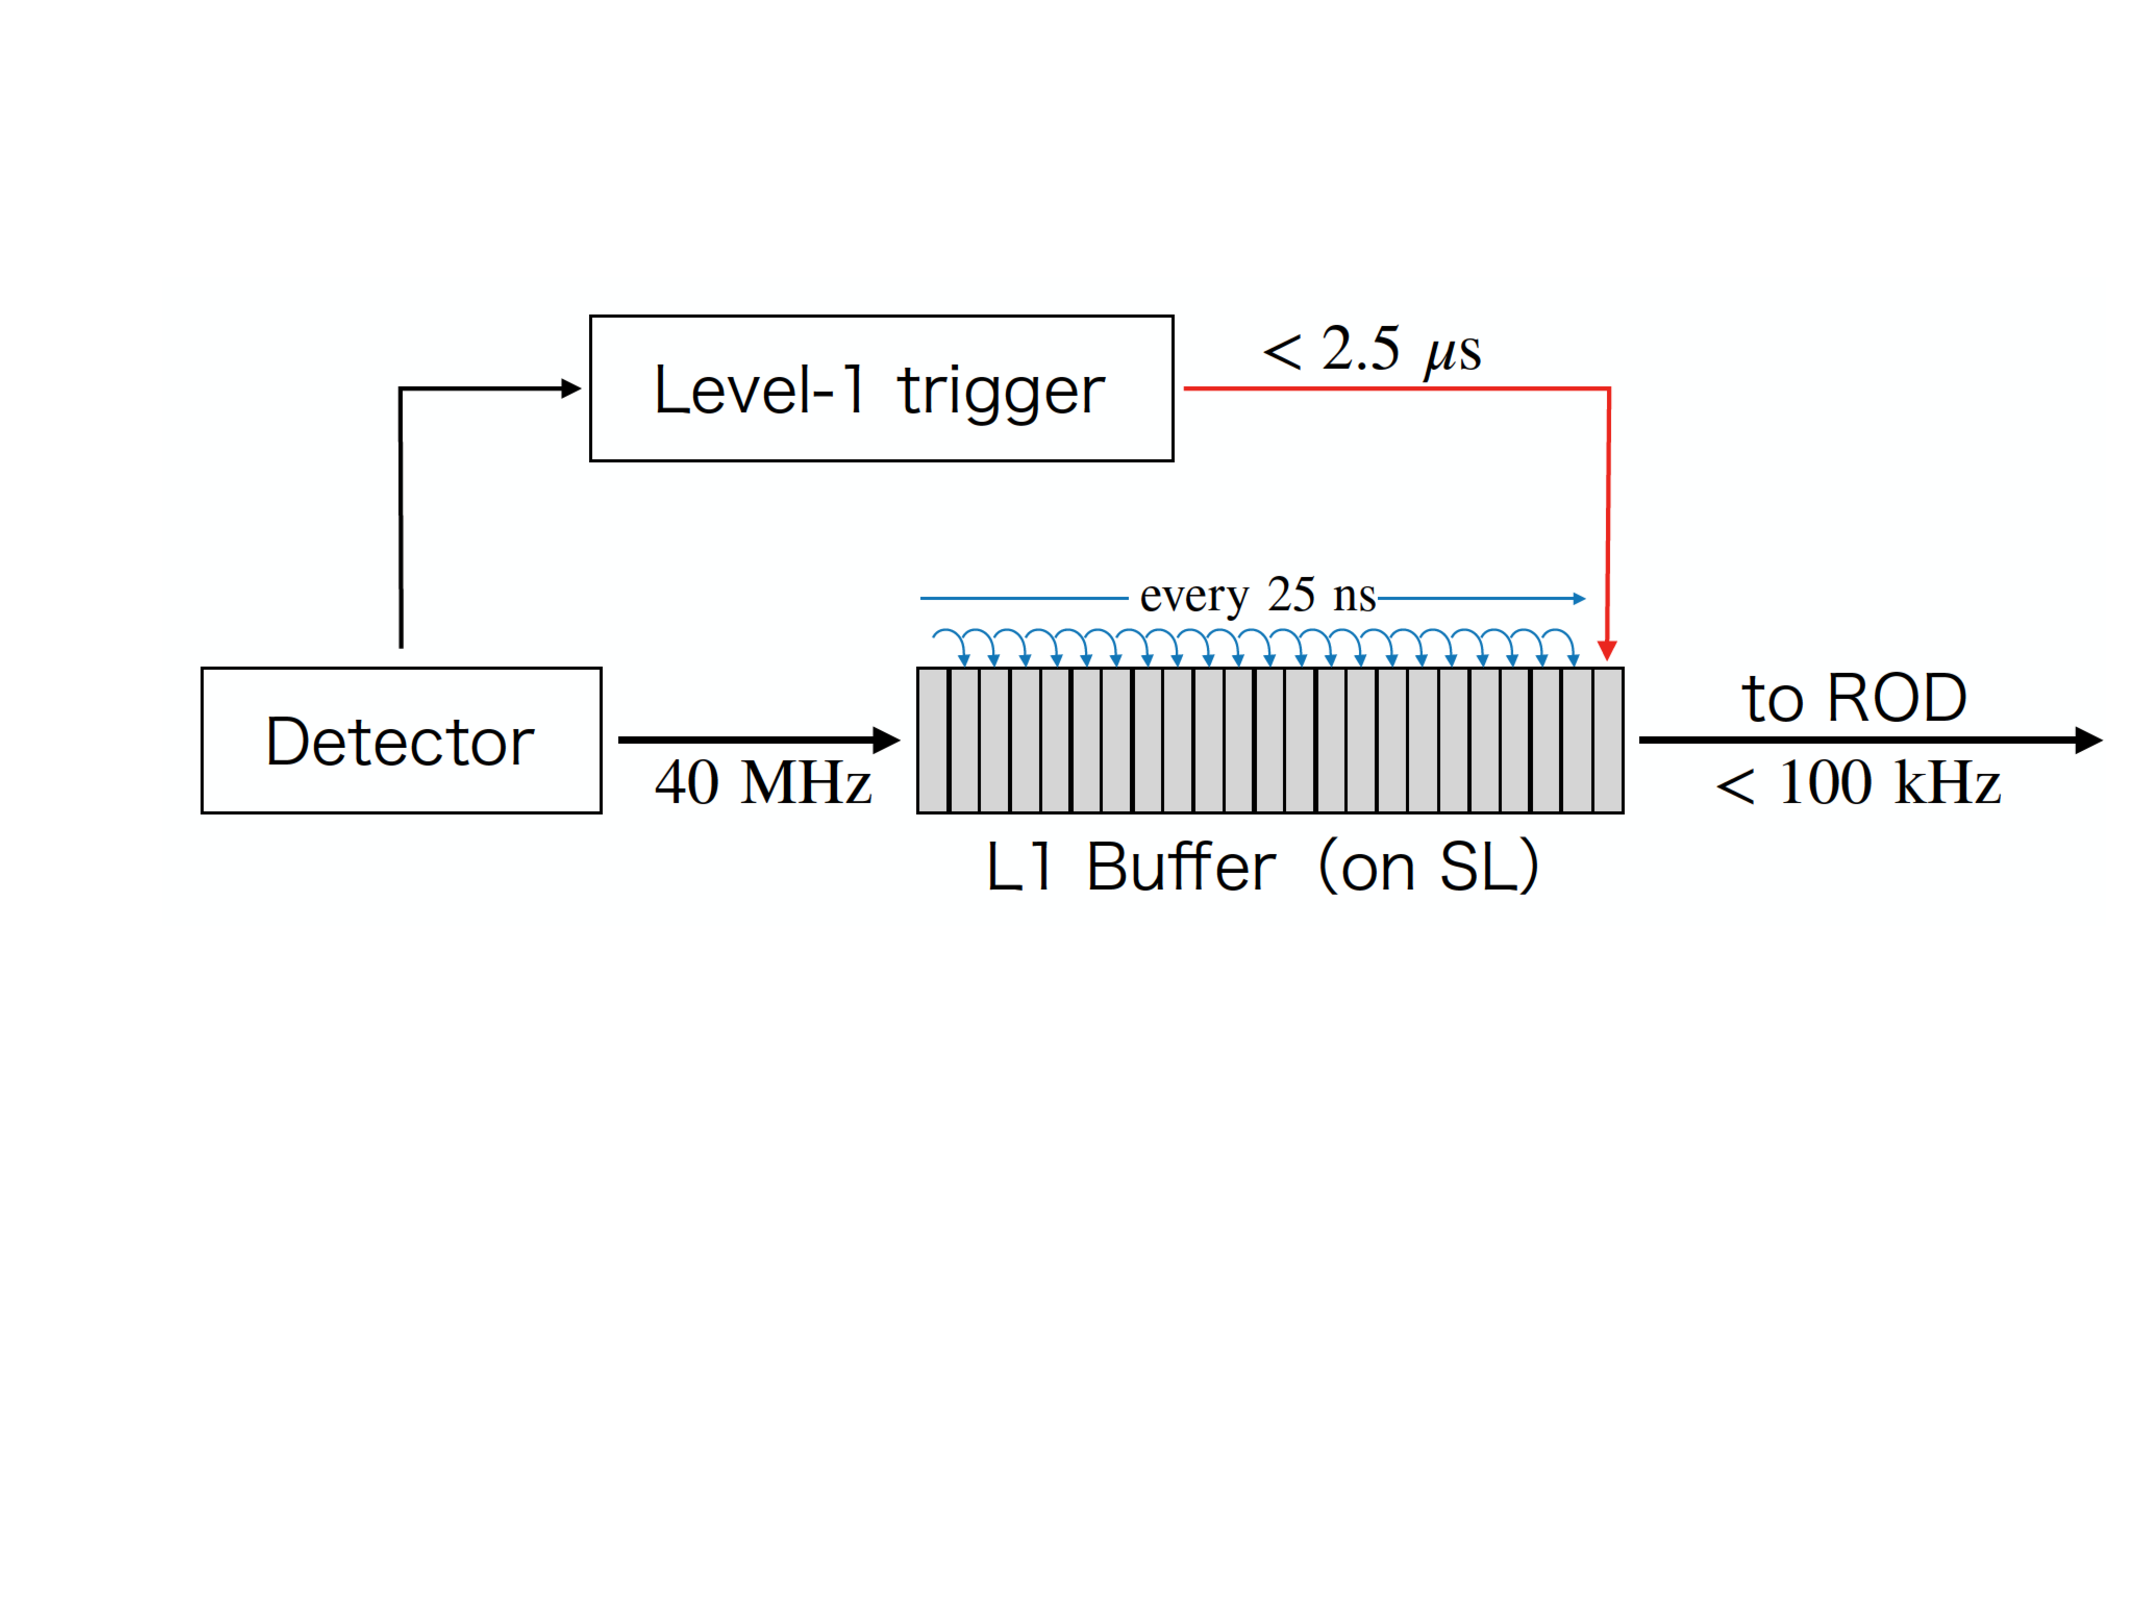
\includegraphics[width=0.95\textwidth,page=1]{img/pdf/pipe.pdf}
        \caption[L1~におけるトリガーシステムの詳細]{L1~におけるトリガーシステムの詳細。40~MHz~での検出器からの情報は~L1~バッファに一時的に保持され、L1~トリガーでの信号の出力を受けたのち、順番に~ROD~へと送信される。}\label{fig:pipe}
\end{figure}
L1~でのトリガー処理はトリガー用ミューオン検出器~(RPC,~TGC)~およびカロリメータによって行われる。それぞれの検出器によって検出された~40~MHz~の頻度で繰り返される陽子バンチ衝突からのヒット信号は、25~ns~おきにL1~バッファに保持され、トリガー処理は情報が保持されている間に行われる。L1~の判定には最大$2.5~\mu\rm{s}$の時間がかかるため、L1~バッファでは最低~100~陽子バンチ分~($25~\rm{ns}\times100=2.5~\mu\rm{s}$)~のデータが保持できるように設定されている。そして決められた遅延時間~(Fixed~Latency)~を経たバンチ衝突のデータに対して、同一のバンチ衝突に対応した~L1~からの信号を受信し、情報の読み出しが行われる。以上のようなトリガー処理システムをパイプライントリガーと呼ぶ。L1~でのイベントの許容レートは~100~kHz~までに設定されており、以上のシステムを通じて~40~MHz~から~100~kHz~以下にまでレートを削減する。

カロリメータおよびミューオン検出器における~L1~の流れについて説明する。カロリメータトリガーでは電子やジェット等の中から高いエネルギーを持つ事象、ミューオントリガーでは高い運動量のミューオンヒットを持つ事象に対してトリガーを行う。L1~は、カロリメータの情報を用いて発行されるトリガー~(L1Calo)、ミューオン検出器の情報を用いて発行されるトリガー~(L1Muon)、それらを組み合わせた複合的なトリガー~(L1Topo)~の~3~種類に分類される。ミューオントリガーではバレル領域とエンドキャップ領域で別々に処理が行われ、L1Muon~の情報は~Muon~to~CTP~Interface~(MUCTPI)~でまとめられる。
そして~L1Calo~と~MUCTPI~でまとめられた~L1Muon~の情報は、Central~Trigger~Processor~(CTP)~へと渡され、それぞれ処理が行われる。

また、L1Calo~と~L1~Muon~の情報は同時に~L1Topo~に送信され、複合的な情報処理が行われる。
L1Topo~においては~L1Calo~と~L1Muon~のトリガーアイテムを組み合わせたトリガーが発行できるだけでなく$\eta$方向、$\phi$方向の位置情報を用いて不変質量を組み、粒子の共鳴に由来することの要求も行うことができる。そして、L1Topo~で処理された情報についても、L1Muon~や~L1Calo~と同様に~CTP~へと送信される。

L1Calo,~L1Muon~および~L1Topo~の情報は、以上の流れから~CTP~に集められ、~512~個の候補選別アルゴリズムを介して事象選別される。CTP~でのトリガー判定によりデータ読み出しが認められた信号に対しては~L1A~(Level-1~Accept)~が発行される。発行された~L1A~は~40~MHz~のクロックとともに~Timing~Trigger~and~Control~(TTC)~システムを経由して各測定器の読み出しシステムに送信される。

L1A~が発行された事象の信号は、情報の読み出しおよび保存を行うために~Read-Out~Driver~(ROD)~に送信される。このときデータは圧縮され、信号情報とともにバンチ交差識別番号~(BCID)~が付与される。BCID~は、LHC~の~25~ns~毎のバンチ衝突に対して、どのバンチに対応しているのかを識別する役割を持つ。ROD~は収集したデータをイベントごとに処理し、BCID~の整合性を確認したのち~Simple~Link~Interface~(S-LINK)~\cite{URL:20}を通して、Read-Out~System~(ROS)~へと情報を送信する。

また、初段トリガーが発行された周辺の位置情報~(Region~of~Interest:~RoI)~は、後段トリガーに渡され事象選別の種として利用される。

\subsubsection{初段トリガーにおけるタイミング合致の重要性}
前節で述べたように~L1~ではパイプライントリガーと呼ばれるシステムを採用している。このトリガーシステムにおいては、異なる検出器ごとの情報を同一のバンチ衝突ごとに対応させ、正しく一致させることが非常に重要となる。検出器は衝突点から最大で約~20~m~の距離に設置されており、ミューオンの検出器到達には最大で約~100~ns~程の時間がかかる。各検出器でのタイミングをそろえるためには詳細な調整が必須である。L1Muon~および~L1Calo~では、各検出器に対し粒子がほぼ光速で到達するということを仮定した上で、基準に定めた陽子バンチ衝突による生成粒子の信号と判断した場合にトリガー判定を行っている。本論文では、トリガー判定を行う上で基準に定められたバンチのことを基準バンチ~(Current~Bunch)~と呼ぶこととする。L1Muon~や~L1Calo~では、基準バンチ由来ではないと考えられるタイミングでの入力情報に対しては、トリガー判定を行うことができない。一方複合的なトリガーである~L1Topo~においては、基準バンチの情報に加えてその次のバンチの情報を組み合わせたトリガー判定を行うことが可能である。本論文では、基準バンチの次の陽子バンチ衝突のことを次バンチ~(Next~Bunch)、また基準バンチの前の陽子バンチ衝突のことを前バンチ~(Previous~Bunch)~と呼ぶ。

以上のように正しくトリガー処理を行うには各検出器において同一バンチの事象を取得することが非常に重要である。

\subsection{後段トリガー}
後段トリガー~(HLT)~では、初段トリガーで出力された~RoI~を種として、ソフトウェアベースのアルゴリズムでオフライン解析に近い粒子の再構成を行う。HLT~では内部飛跡検出器および~MDT~や~CSC~などの精密測定用ミューオン検出器、L1Calo~におけるカロリメータなどの情報を用いて、飛跡再構成および$E_{\rm{T}},~p_{\rm{T}}$の計算をする。L1~で~100~kHz~にまで落とされたイベントレートを~HLT~では数~kHz~にまで削減する。

HLT~は~L1~とは異なり、数~10~ms~から~1~s~程の長い計算時間によってより詳細にトリガー判定を行う。また大量のコンピューティングファーム利用することで精密で膨大な計算を並行して処理することができる。HLT~のアルゴリズムは~Processing~Unit~(PU)~と呼ばれる約~40,000~個のアプリケーションで実行される~\cite{AR:15}。各~PU~は一つの事象を数~100~ms~以内に処理できるように設計されている。PU~の一連の処理においては複数の特徴抽出アルゴリズムが実行される。HLT~において事象がアクセプトされるとオフライン再構成のためにデータを一時ストレージへ送信し、最終的には~CERN~コンピューティングセンターの大規模ストレージシステムに保存する。

\chapter{重い長寿命荷電粒子の探索とトリガー}
\thispagestyle{empty}
\label{chap:3}
LHC~は~重心系エネルギー~13~TeV~の陽子陽子衝突により新粒子を作り出すことで原子宇宙の謎に迫っている。ヒッグス粒子の詳細な性質の解明や暗黒物質などに答えを与えうる超対称性粒子の探索は、標準模型を超えた物理の検証の一つとして盛んに行われている。
本研究では、新物理探索の一つである超対称性理論から導き出される重い長寿命荷電粒子の探索について説明する。

\section{標準模型を超える物理}
\label{sec:BSM}
\chapref{chap:1}で述べた標準模型はこれまでの素粒子物理を高精度で説明する理論である。しかし、発見されたヒッグス粒子の質量が~125~GeV~(陽子質量の約~125~倍)~である理由やクォークとレプトンがそれぞれ~6~種類ずつおよびゲージボソンが~3~種類という多様な粒子から構成される理由などの疑問は未だ解決できていない。これらの疑問に答えうる一つの理論が大統一理論~(Grand~Unified~Theory:~GUT)~である~\cite{AR:10}。\figref{fig:gut}に~GUT~の概念図を示す。GUT~は、電磁相互作用、弱い相互作用および強い相互作用を統一する理論である。GUT~では、あるエネルギースケール~(GUT~スケール)~で結合定数を一致させる必要がある。このエネルギースケールはおよそ~1016~GeV~であると見積もられている。一方で電弱相互作用のエネルギースケールは~102~GeV~であるため、~GUT~スケールとは大きな差異がある。これを階層性問題と呼ぶ~\cite{AR:06}。また、階層性問題に派生してヒッグス粒子の質量に関しても問題が生じる。これは微調整問題と呼ばれる~\cite{AR:06}。輻射補正を考慮したヒッグス粒子の質量は、\equref{eq:higgs}で表される。
\begin{align}
    m_{H}^2=m_{H}^2(\rm{tree})+\mathcal{O}(\Lambda^2) \label{eq:higgs}
\end{align}
右辺は~tree~レベルと輻射補正を考慮した項に分けた。$\Lambda$は切断パラメータと呼ばれ、標準模型が有効となるスケールの上限である。左辺のヒッグス粒子の質量は電弱スケールであるのに対し、右辺の$\Lambda$は~GUT~スケールであるため、明らかに両辺で矛盾が生じる。この矛盾を解決するには、$10^{-26}$という精度で微調整する必要があり、非常に不自然である。

\begin{figure}[tb]
        \centering   
        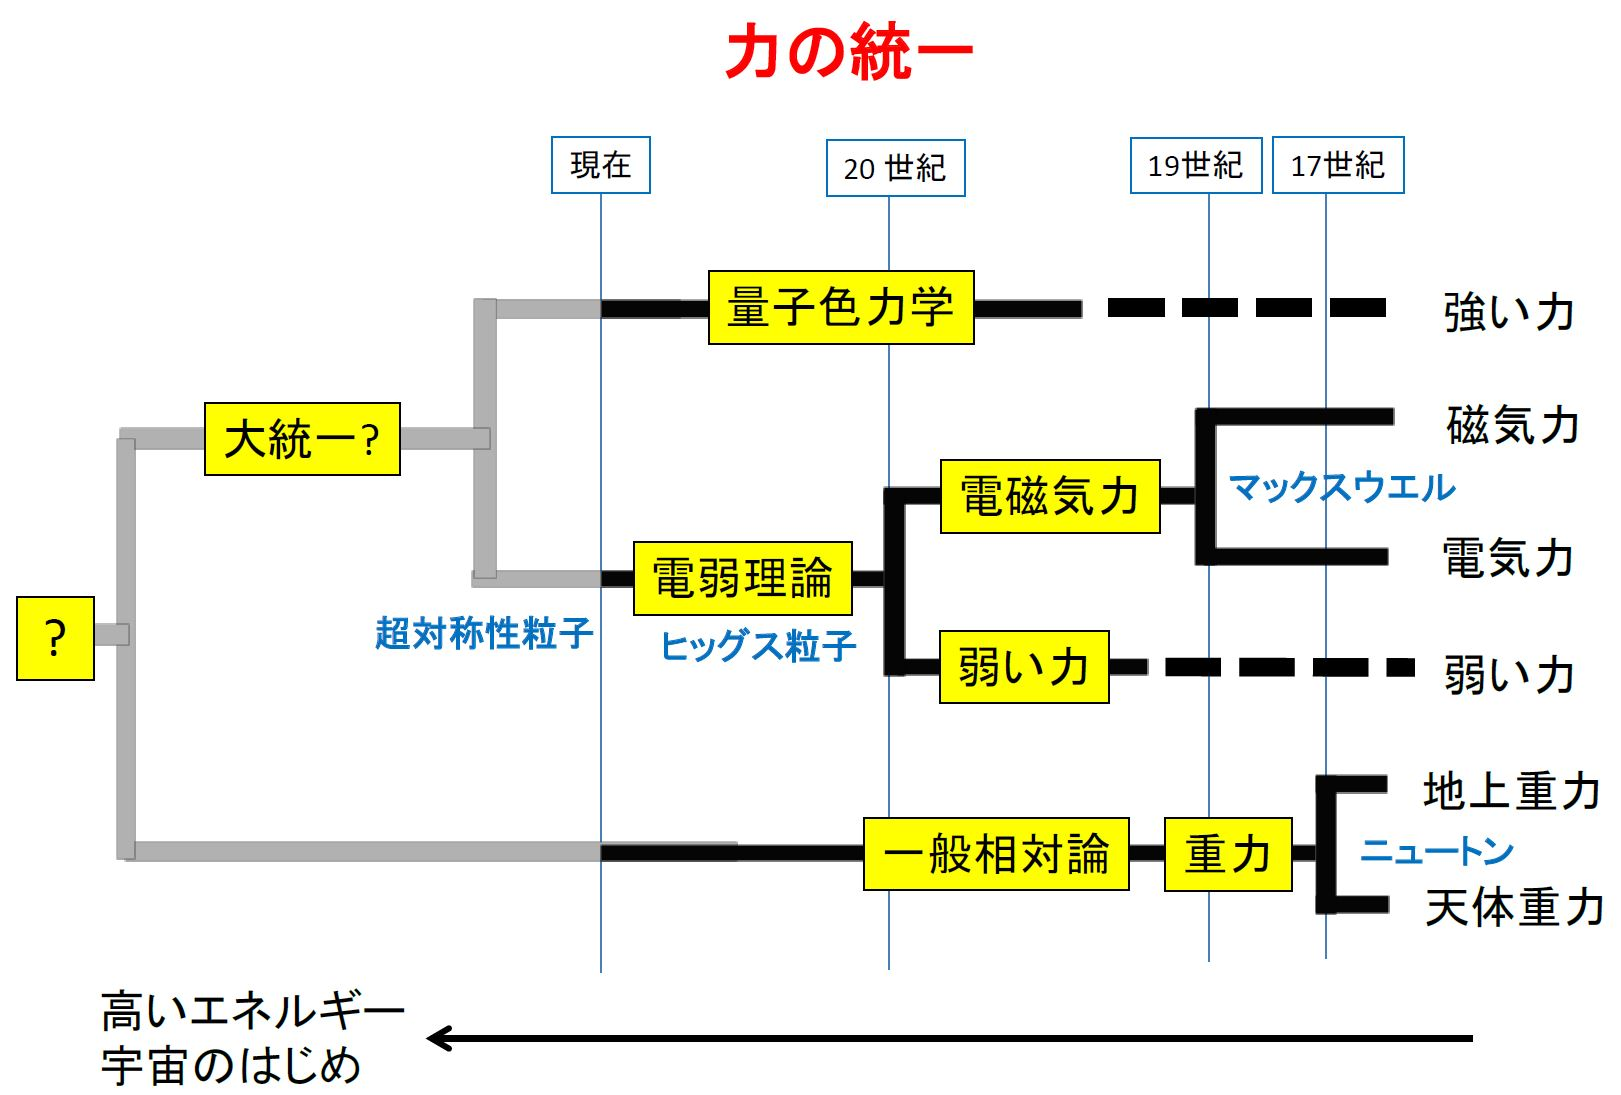
\includegraphics[width=0.9\textwidth]{img/jpeg/physics_bsm_05.jpg}
        \caption[力の統一を表した概念図]{力の統一を表した概念図~\cite{URL:01}。大統一理論は、電磁相互作用、弱い相互作用および強い相互作用を統一する理論である。}\label{fig:gut}
\end{figure}


さらに、標準模型では説明できない事象の一つとして暗黒物質の存在がある~\cite{AR:11}。暗黒物質は銀河の回転速度の観測からその存在が予言された。質量分布が球対称であることを仮定すると、中心からの距離$r$の位置での回転速度$v$は、\equref{eq:dark}と表現できる。
\begin{align}
    v^2\propto\frac{M(r)}{r} \label{eq:dark}
\end{align}
ここで$M~(r)~$は半径$r$内の全質量を表す。もし銀河が現在観測可能な物質のみで構成されているとするならば、その速度$v$は距離$r$とともに小さくなることが示唆される。しかし、近年の銀河の回転速度の観測結果により速度が減少していないことが分かっている~\cite{AR:16}。これは我々が未観測な物質、すなわち暗黒物質が存在する証拠である。現在の宇宙観測によれば、宇宙には光を発していない暗黒物質が通常の物質の~5~倍以上ものエネルギーを担って存在していることが判明している。これは宇宙の全エネルギーの約$22\%$である。

このような標準模型では説明できない物理を、標準模型を超えた物理、~Beyond~the~Standard~Model~(BSM)~と呼び、ATLAS~実験をはじめとして世界中で~BSM~の発見を目的に実験が行われている。そして標準模型における諸問題を解決するための有力な理論の一つとされているのが超対称性理論である。

\section{超対称性理論}
超対称性~(Supersymmetry:~SUSY)~とは、ボソンとフェルミオン間の対称性である~\cite{AR:12,AR:12a}。この対称性は、\secref{sec:BSM}で述べた~標準模型における問題を説明できる非常に興味深い理論である。最小超対称標準模型~(Minimal~Supersymmetric~Standard~Model:~MSSM)~では、標準模型粒子~(SM~粒子)~のそれぞれに対して、超対称性粒子~(SUSY~粒子、スーパーパートナー)~が存在する~\cite{AR:12b}。標準模型ではヒッグス粒子は~1~つであるのに対し、MSSM~ではヒッグス粒子のパートナーであるヒッグシーノは複数存在する。また、光子、$W/Z$ボソンおよびヒッグス粒子のスピン~1/2~のスーパーパートナーは、混合してニュートラリーノ$\Tilde{\chi}^0$とチャージーノ$\Tilde{\chi}^{\pm}$と呼ばれる質量固有状態を与える。グラビティーノは重力を伝えるボソンと考えられている重力子~(グラビトン)~のスーパーパートナーである。\tbref{tb:SUSY}に~SUSY~粒子の一覧を示した。

SM~粒子と~SUSY~粒子には大きく~2~つの違いがある。1~つはスピンである。SM~粒子に対し、SUSY~粒子はスピンが$1/2$ずれただけで、電荷などは等しい。SM~でのフェルミオンに対するスーパーパートナーにはスフェルミオンが対応する。SM~におけるボソンに対してはボシーノが対応する。もう~1~つの違いは質量である。SUSY~粒子は未発見のため、超対称性理論は少なくとも低エネルギー領域では破れていると考えられている。したがって、SUSY~粒子は~SM~粒子より大きいオーダーでの質量を持ち、非常に重いと考えることが一般的である。

超対称性理論では、\equref{eq:Rparity}のように表される$R$-パリティと呼ばれる対称性を仮定している。
\begin{align}
    R = (-1)^{3(B-L)+2S} \label{eq:Rparity}
\end{align}
$S$はスピン、$B$はバリオン数、$L$はレプトン数を示している。
$R$-パリティは、SM~粒子に正、SUSY~粒子に負を付与する対称性である。$R$-パリティが保存する場合、SUSY~粒子は、自身の質量より軽い~SUSY~粒子と~SM~粒子に崩壊する。このとき、最も質量の軽い~SUSY~粒子~(Lightest~SUSY~Particle:~LSP)~は安定となる。LSP~が~SUSY~粒子におけるどの粒子であるかはモデルによって様々だが、電気的に中性なニュートラリーノやグラビティーノであれば~LSP~は暗黒物質の候補となる。$R$-パリティが保存しない場合、LSP~はより軽い~SM~粒子へと崩壊する。$R$-パリティが破れることを$R$-Parity~Violation~(RPV)~と呼ぶ~\cite{AR:12g}。
\figref{fig:GUT}~に示すように、SUSY~を仮定することで\secref{sec:BSM}で述べた大統一理論における~3~つの結合定数は~GUT~スケールで一致する。

\begin{table}[tbp]
	\centering
	\begin{tabular}{c|c|ccc|c|c} \hline
	& &\multicolumn{3}{c|}{世代}& \multirow{2}{*}{スピン} & \multirow{2}{*}{電 荷} \\
	& &第1&第2&第3&  &  \\ \hline
	\multirow{4}{*}{スフェルミオン} & \multirow{2}{*}{スクォーク} & $\Tilde{u}$ & $\Tilde{c}$ & $\Tilde{t}$ & 0 & +2/3 \\
	&  & $\Tilde{d}$ & $\Tilde{s}$ & $\Tilde{b}$ & 0 & -1/3 \\ \cline{2-5}
	& \multirow{2}{*}{スレプトン} & $\Tilde{\nu_e}$ & $\Tilde{\nu_{\mu}}$ & $\Tilde{\nu_{\tau}}$ & 0 & 0 \\
	&  & $\Tilde{e}$ & $\Tilde{\mu}$ & $\Tilde{\tau}$ & 0 & -1 \\ \hline\hline
	\multirow{5}{*}{ボシーノ} & ニュートラリーノ& \multicolumn{3}{c|}{\multirow{2}{*}{$\Tilde{\gamma},~\Tilde{Z}^0,~\Tilde{H}^{0}_1,~\Tilde{H}^{0}_2$}}& \multirow{2}{*}{1/2} & \multirow{2}{*}{0} \\
	&~($\Tilde{\chi}^0$)~&  &  & & & \\ \cline{2-5}
	& チャージーノ& \multicolumn{3}{c|}{\multirow{2}{*}{$\Tilde{W}^{\pm},~\Tilde{H}^{\pm}$}} & \multirow{2}{*}{1/2} & \multirow{2}{*}{$\pm1$} \\
	& ~($\Tilde{\chi}^{\pm}$)~ & &&&& \\ \cline{2-5}
	& グルイーノ & \multicolumn{3}{c|}{$\Tilde{g}$} & 1/2 & 0 \\ \cline{2-5}
	& グラビティーノ & \multicolumn{3}{c|}{$\Tilde{G}$} & 3/2 & 0 \\ \hline
	\end{tabular}
	\caption[超対称性粒子の一覧]{超対称性粒子の一覧~\cite{AR:12}。}
	\label{tb:SUSY}
\end{table}

\begin{figure}[tbp]
        \centering   
        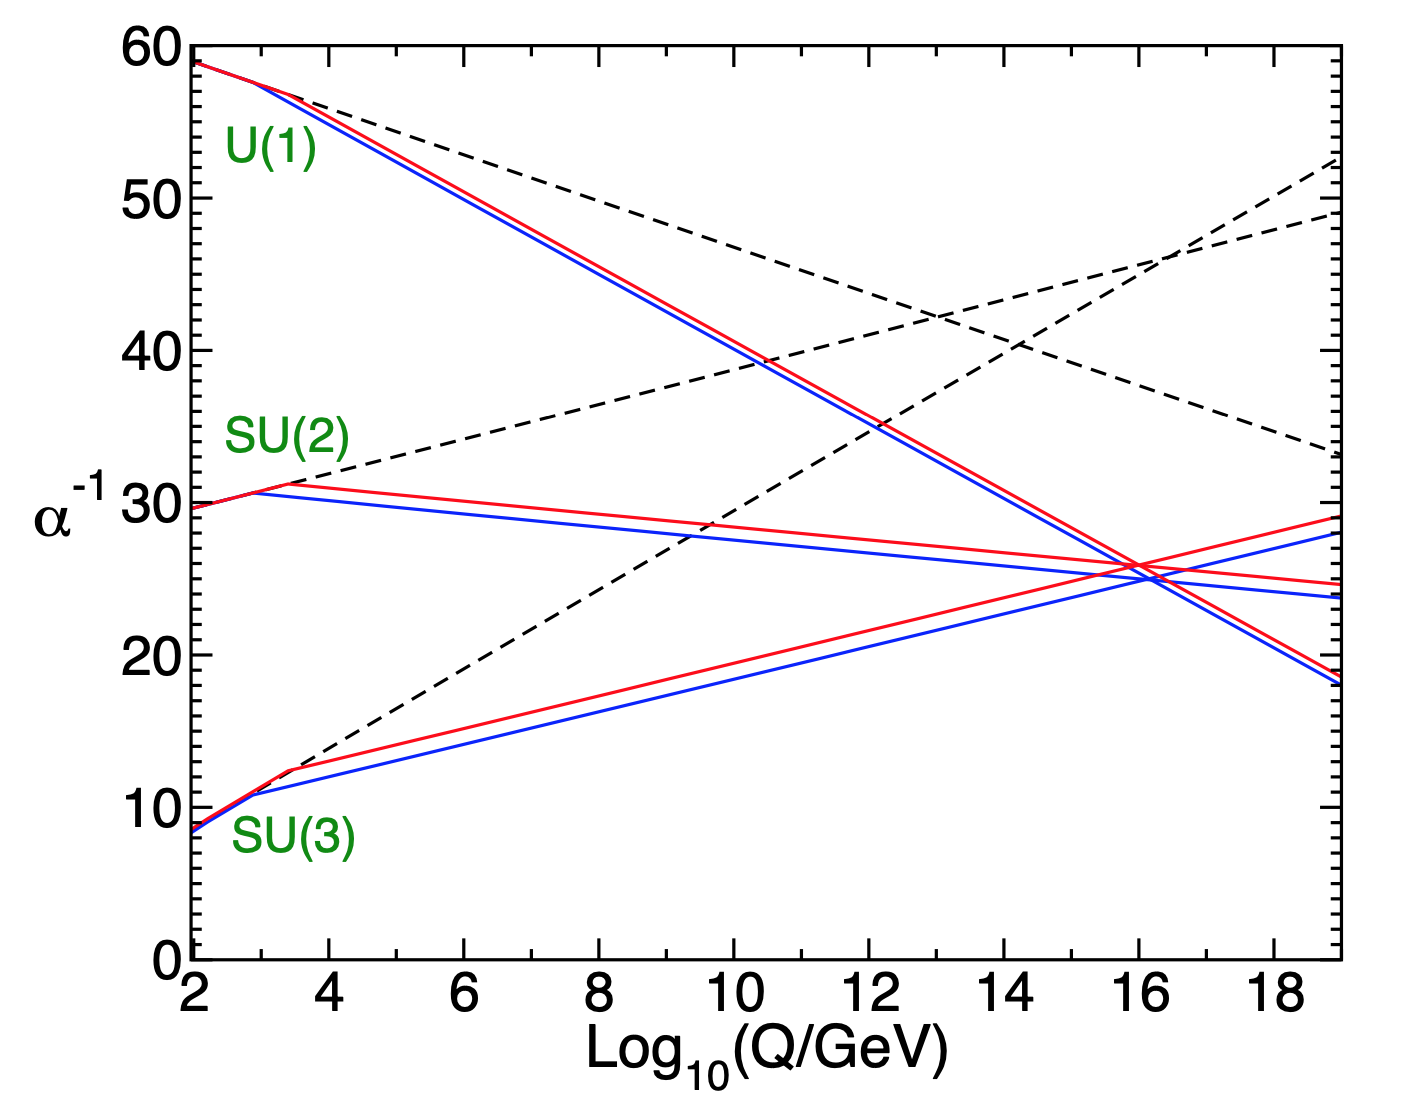
\includegraphics[width=0.85\textwidth]{img/pdf/gut.png}
        \caption[各相互作用における結合定数とエネルギーの関係]{各相互作用における結合定数とエネルギーの関係~\cite{AR:01} 。破線は~SM、実線は~MSSM~を示している。U(1)、SU(2)、SU(3)はゲージ対称性を表し、それぞれ電磁相互作用、弱い相互作用、強い相互作用に対応する。}
        \label{fig:GUT}
\end{figure}

また~SUSY~の枠組みでは$\rm{tan}\beta$という自由パラメータが本質的に重要な働きをする~\cite{URL:24}。SUSY~では~2~種類のヒッグス粒子$\left(H_{\rm{u}}^0,~H_{\rm{d}}^0\right)$が導入され、$\sqrt{v_{\rm{u}}^2~+~v_{\rm{d}}^2}~=~v$を満たしたそれぞれの真空期待値$(v_{\rm{u}},~v_{\rm{d}})$によって電弱対称性が破れる。$v$は標準模型でのヒッグスの真空期待値を表す。この真空期待値の比を\equref{eq:tan}と定義する。
\begin{align}
    \rm{tan}\beta~=~\frac{\it v_{\rm{u}}}{\it v_{\rm{d}}} \label{eq:tan}
\end{align}
SUSY~におけるゲージ結合定数は$\rm{tan}\beta$の関数として記述することができ、SUSY~においては$\rm{tan}\beta$の数値の仮定のもと探索を行う。

\subsubsection{超対称性粒子の探索結果}
超対称性粒子は、ATLAS~実験並びに~CMS~実験において幅広く探索が進められているが、未だ発見には至っていない。しかし、現在までの~SUSY~探索により~SUSY~粒子には大きな制約が課せられ、存在が許される粒子の質量領域が少なくなってきている。\figref{fig:susy1}は、ATLAS~の様々な~SUSY~探索における除外質量制限を示している~\cite{AR:13e}。グルイーノの生成においては約~2.3~TeV、第一世代および第二世代におけるスクォークにおいては約$\rm{600~GeV\sim1.9~TeV}$、第三世代のスクォークにおいては約$\rm{600~GeV\sim1.2~TeV}$、電弱ゲージーノでは約$\rm{400\sim1100~GeV}$、スレプトンの生成においては約$\rm{700~GeV}$までの質量制限を課している。

\begin{figure}[tbp]
        \centering   
        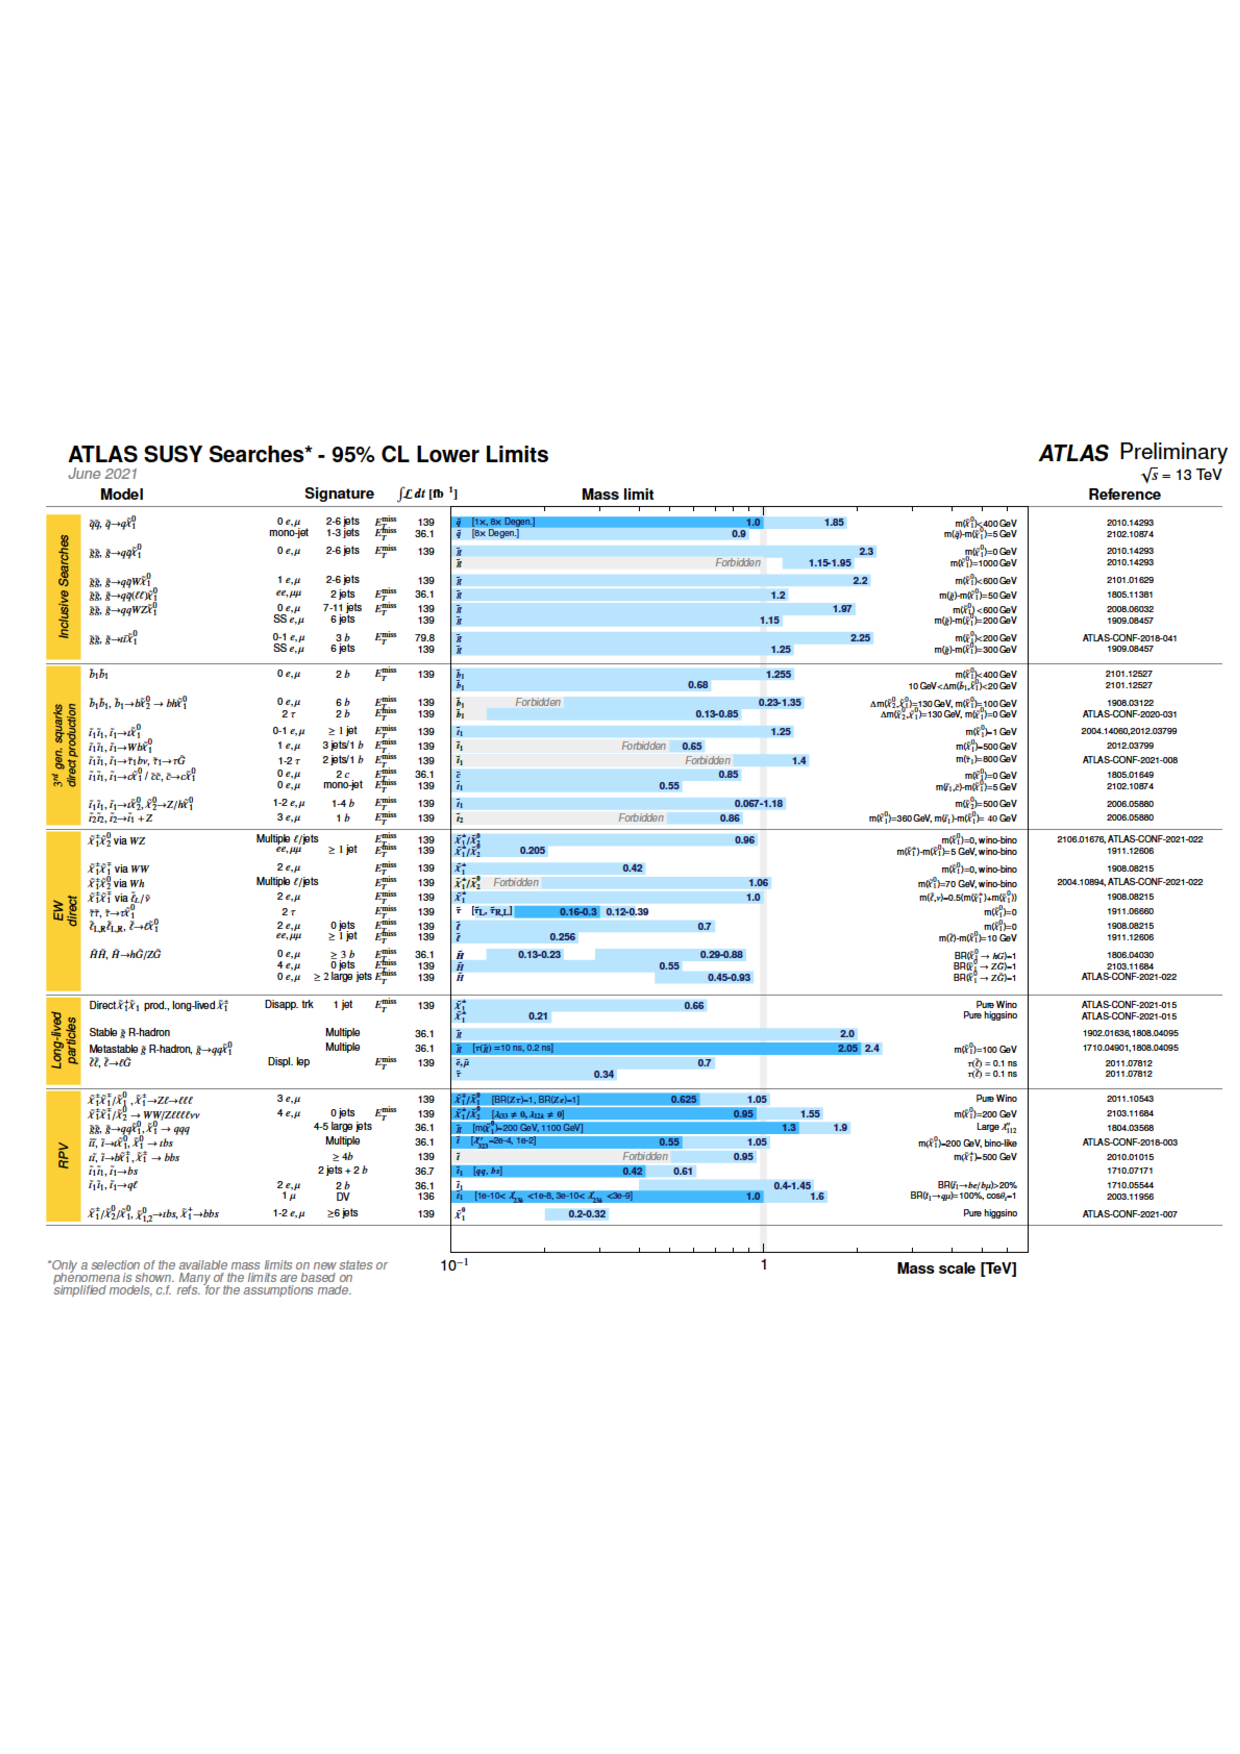
\includegraphics[width=\textwidth,page=1]{img/pdf/susy1.pdf}
        \caption[LHC~での~SUSY~探索の概要]{LHC~での~SUSY~探索の概要~\cite{AR:13e}。SUSY~における様々な探索と~ATLAS~の除外質量制限を示している。}\label{fig:susy1}
\end{figure}


\subsection{超対称長寿命粒子}
\label{subsec:LSP}
超対称性のモデルのなかには,崩壊が抑制され長寿命となる粒子を含むものが多数ある。例えば、Gauge~Mediated~Supersymmetry~Breaking~(GMSB)~モデルでは、~SUSY~の破れのスケールを考慮して一番軽い超対称性粒子~(LSP)~はグラビティーノとなる。そしてグラビティーノと~SUSY~場の結合は著しく弱いため二番目の軽い超対称性粒子~(Next~to~Lightest~Supersymmetric~Particle:~NLSP)~であるスタウ粒子の寿命が長くなると考えられている~\cite{AR:12d,AR:12e}。

Anomaly~mediation~モデルでは,LSP、~NLSP~がチャージーノになり~質量が縮退し、NLSP~である荷電チャージーノは検出可能な寿命$c\tau~=\mathcal{O}(\rm{1}\sim\rm{10}~\rm{cm})$を持つようになる~\cite{AR:12f}。

またゲージーノの質量は約~1~TeV~であるが、split~SUSY~モデルではスカラー粒子の質量が~1~TeV~より重くなると~生成されたグルイーノの寿命が長くなり、グルイーノが標準モデルクォークと結合して無色化した$R$-ハドロンとよばれる状態になる~\cite{AR:12c}。\figref{fig:dia}に~GMSB,~Anomaly~mediation,~split~SUSY~の各モデルにおいて予測されている粒子崩壊課程の一例を示した。

\begin{figure}[tbp]
	\begin{minipage}{0.49\hsize}
	\centering
    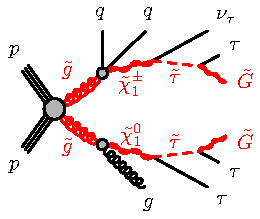
\includegraphics[width=0.7\textwidth]{img/diagram/gogo-qqgtautautauvGG-GMSB.pdf}
    \subcaption{}
    \end{minipage}
    \begin{minipage}{0.49\hsize}
    \centering
    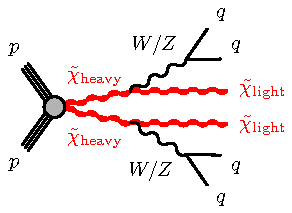
\includegraphics[width=0.7\textwidth]{img/diagram/chichi-qqqq-XX.pdf}
    \subcaption{}
    \end{minipage}\\
    \begin{minipage}{0.98\hsize}
    \centering
    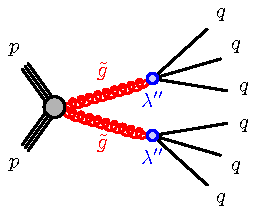
\includegraphics[width=0.35\textwidth]{img/diagram/gogo-3q3q-RPV.pdf}
    \subcaption{}
    \end{minipage}
    \caption[超対称長寿命粒子モデルにおけるファインマンダイアグラムの一例]{超対称長寿命粒子モデルにおけるファインマンダイアグラムの一例~\cite{URL:03}。(a) GMSB モデル。 (b) Anomaly mediation モデル。 (c) split SUSY モデル。}
    \label{fig:dia}
\end{figure}


\subsubsection{重い長寿命粒子の探索結果}
SUSY~における重い長寿命粒子の探索について説明する。\figref{fig:susy2}に~SUSY~における重い長寿命粒子の探索結果を示す。\subsecref{subsec:LSP}で述べた~SUSY~粒子の各モデルにおける様々な探索が行われている~\cite{AR:13a,AR:13b,AR:13c,AR:13d}。
\begin{figure}[tbp]
        \centering   
        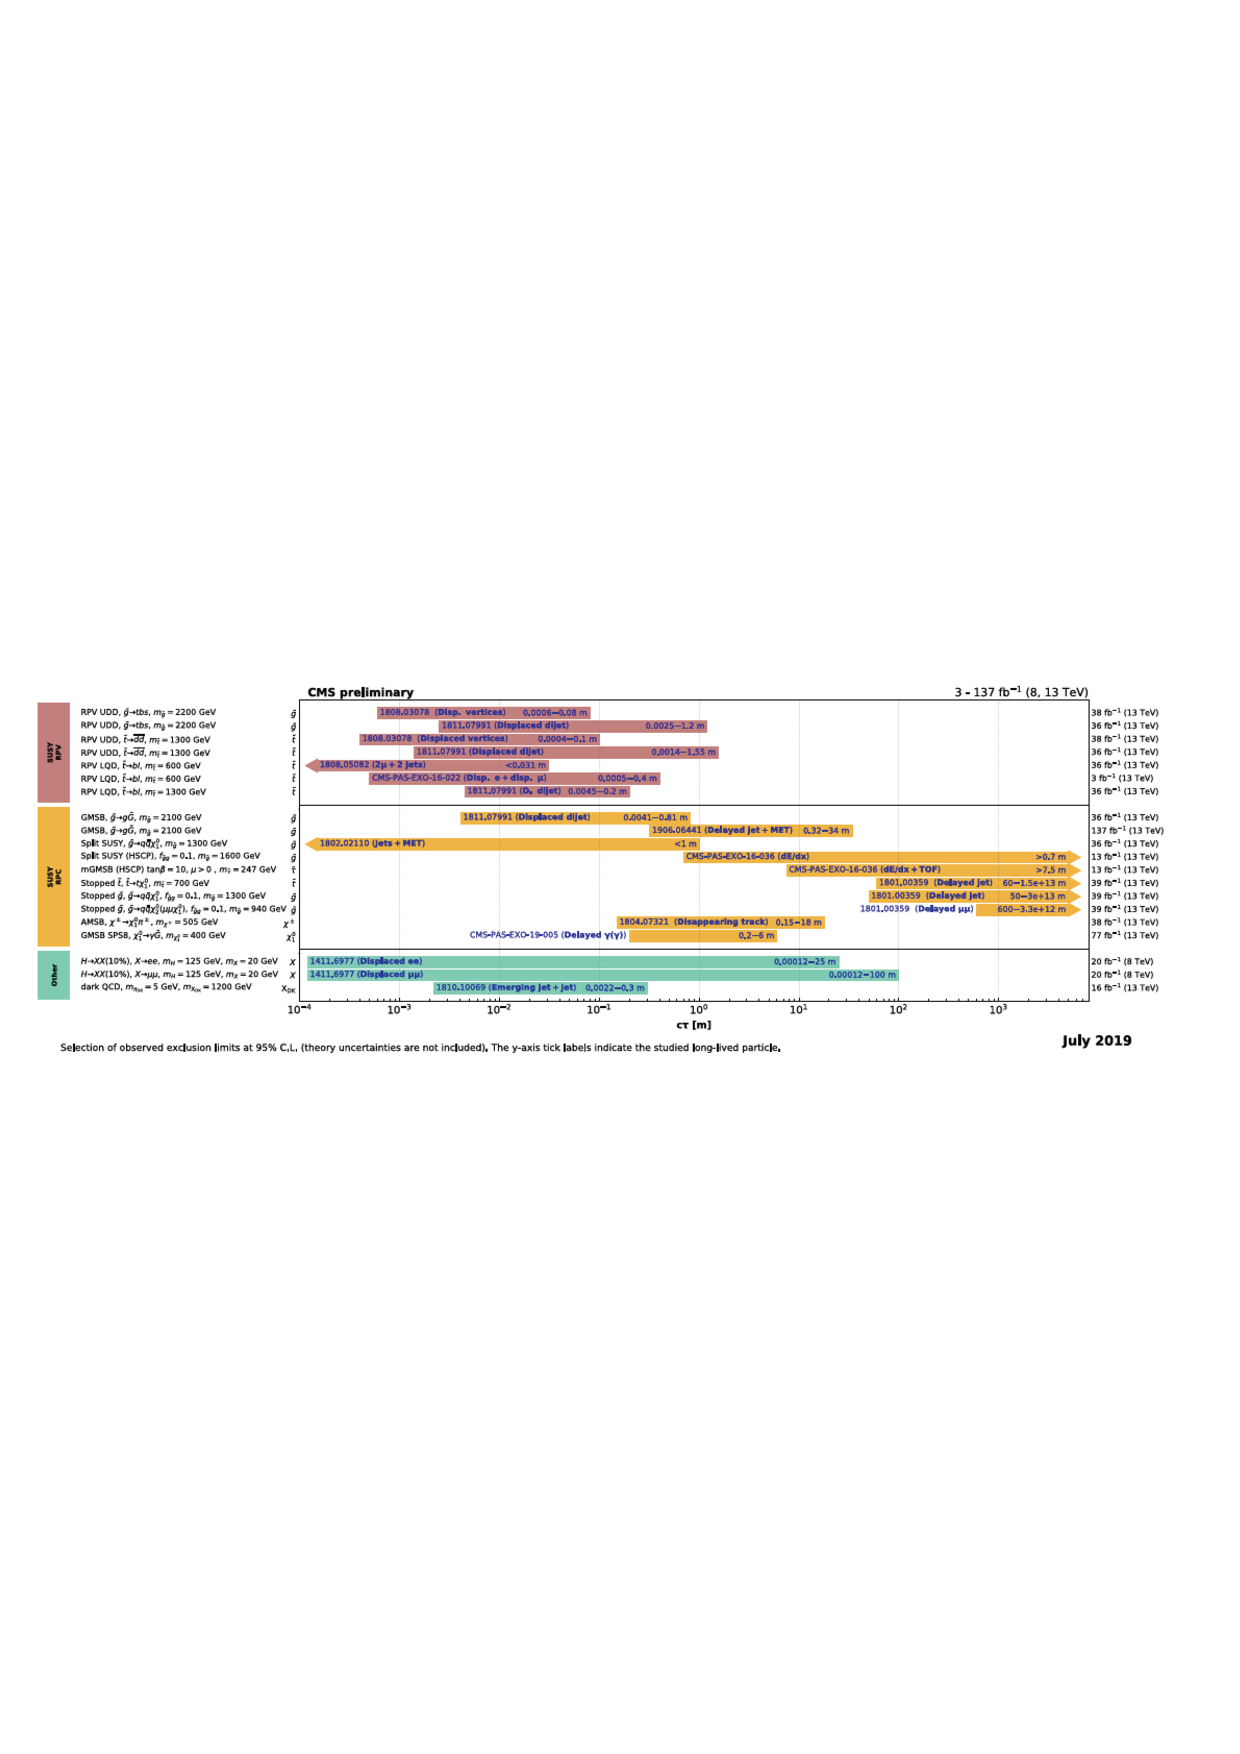
\includegraphics[width=\textwidth,page=1]{img/pdf/susy2.pdf}
        \caption[重い長寿命粒子の探索結果]{重い長寿命粒子の探索結果~\cite{AR:13a,AR:13b,AR:13c,AR:13d}。CMS~によって得られた様々な~SUSY~モデルにおける長寿命粒子の$95\%$信頼区間除外領域。横軸は固有崩壊長~($c\tau$)~。}\label{fig:susy2}
\end{figure}

本論文においては、GMSB~モデルにおいて存在が示唆されている長寿命スタウ粒子の探索結果について紹介する。

ATLAS~実験~Run~1~において収集された重心エネルギー$\sqrt{s}~=~8~\rm{TeV}$での陽子陽子衝突による積算ルミノシティ$19.8~\rm{fb}^{-1}$のデータサンプルを使用して、長寿命スタウ粒子の探索が行われた~\cite{AR:03}。推定されたバックグラウンドを超える過剰は観察されず、質量に制限が課せられた。スタウ粒子は、$\rm{10\sim50}$の$\rm{tan}\beta$に対して$\rm{440\sim385~GeV}$の質量まで除外され、スタウ粒子の直接生成のみが考慮される場合は~290~GeV~までの制限を課すことができている。\figref{fig:stau1}に~GMSB~モデルにおけるスタウ粒子の観測結果を示す。

\begin{figure}[tbp]
    \begin{minipage}{0.49\hsize}
    \centering   
    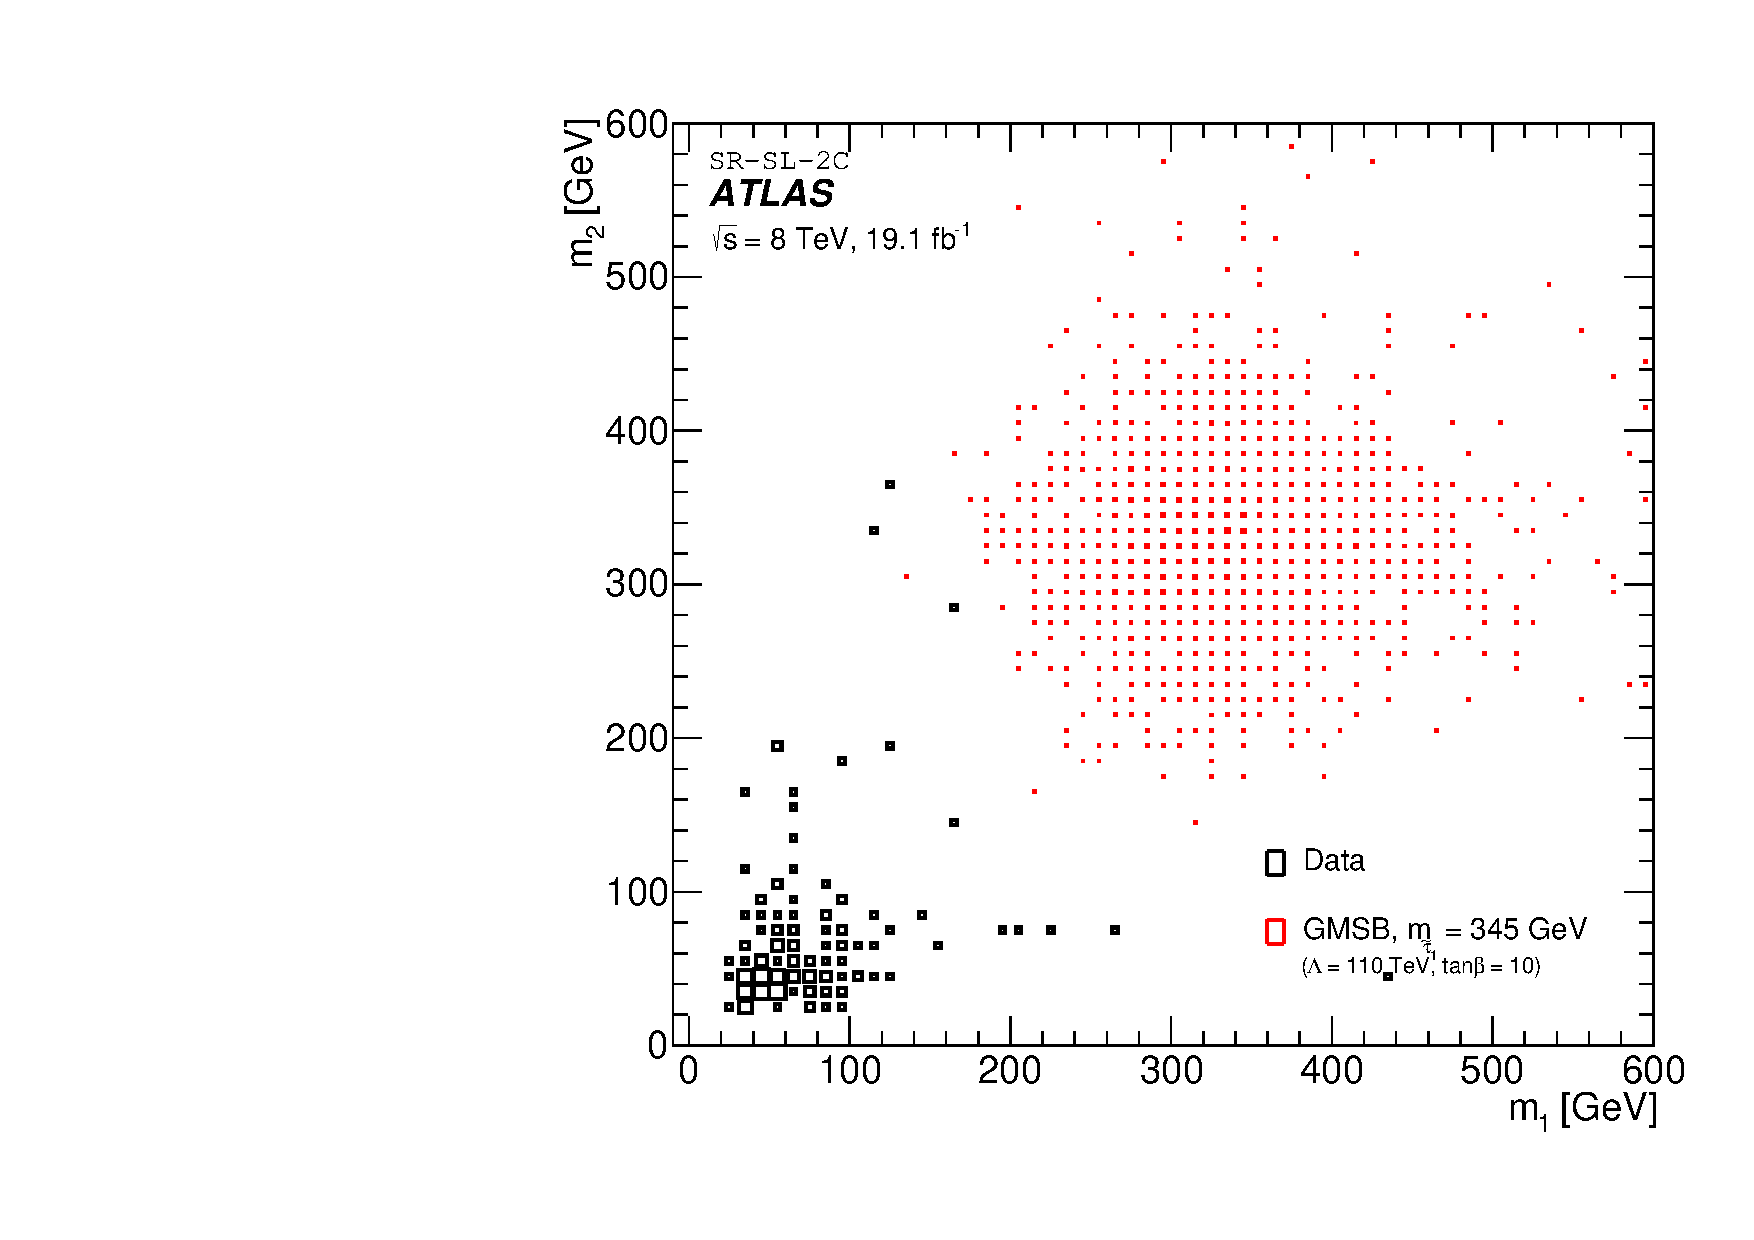
\includegraphics[width=\textwidth]{img/stau/fig_02a.pdf}
    \subcaption{}
    \end{minipage}
    \begin{minipage}{0.49\hsize}
    \centering   
    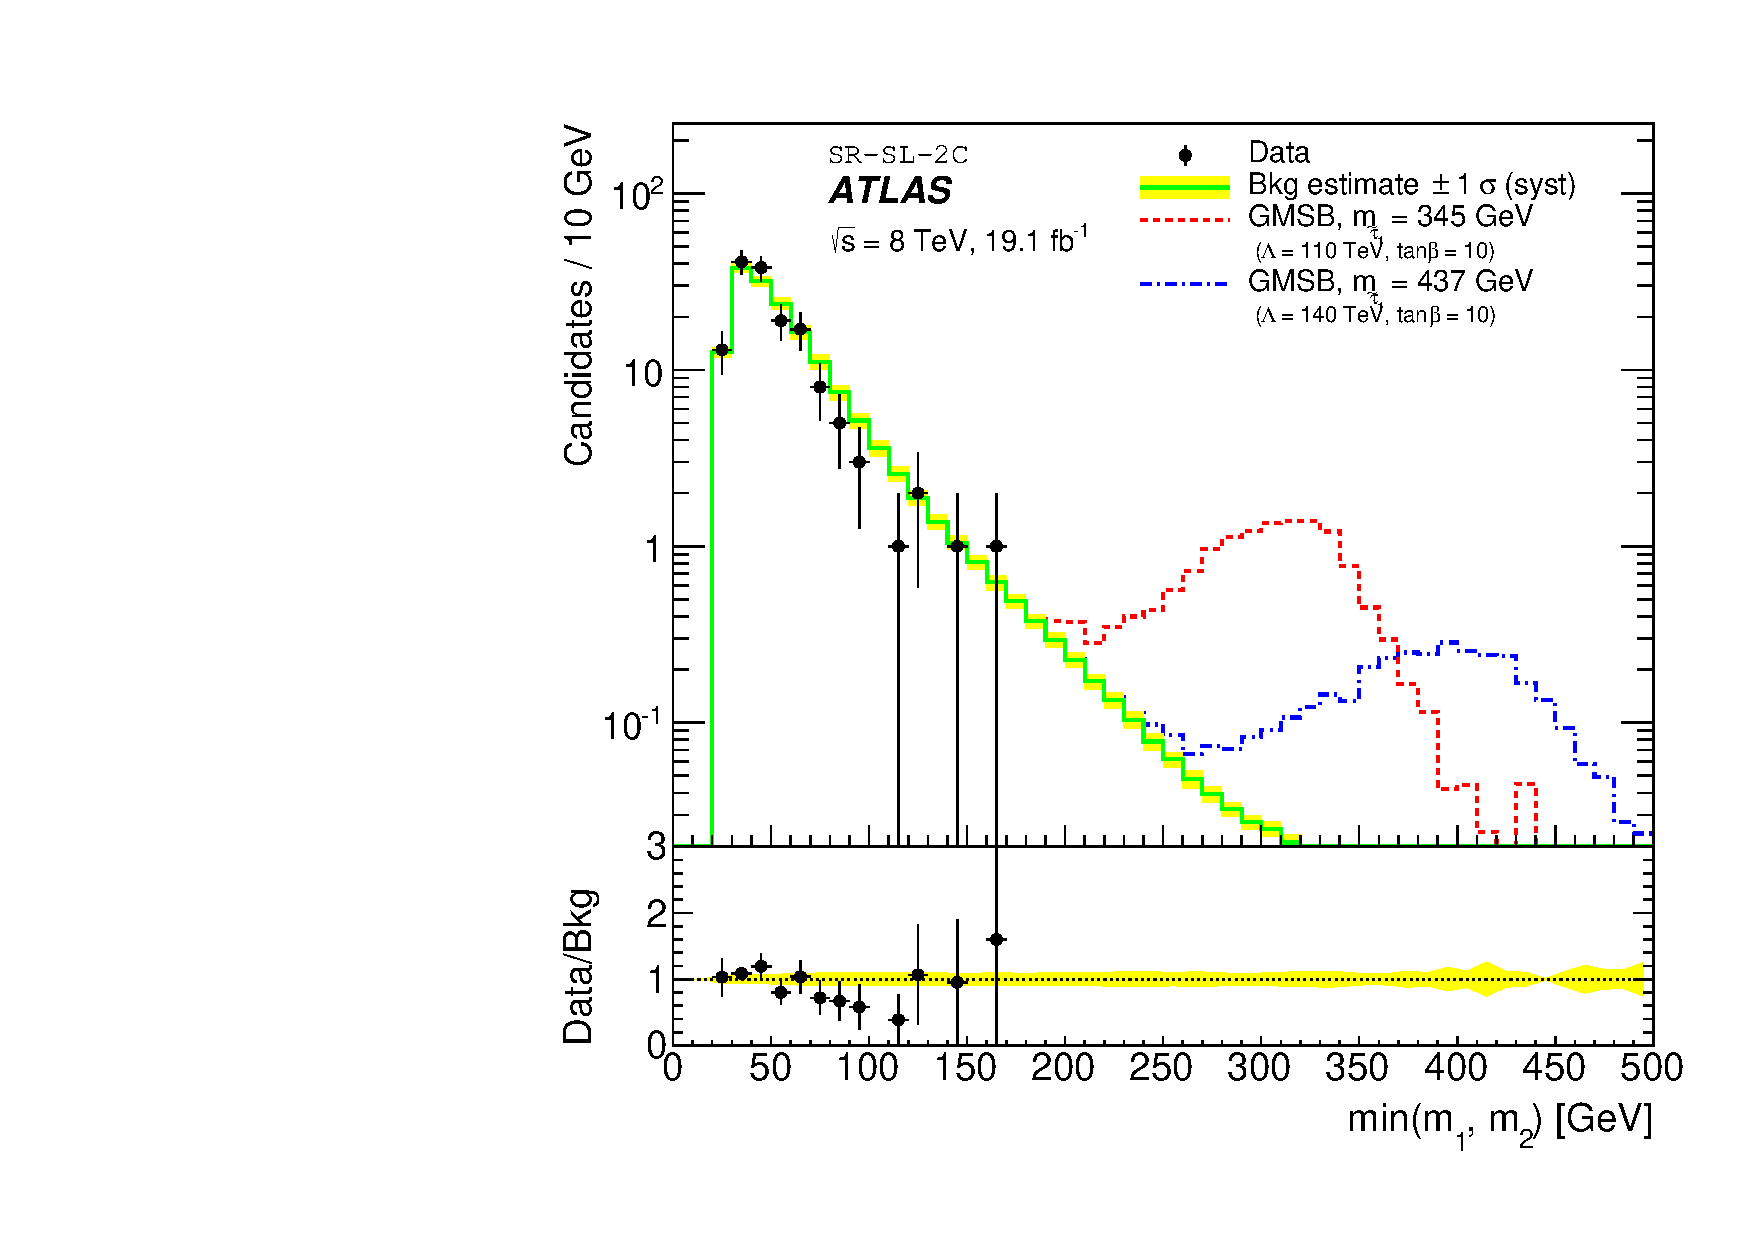
\includegraphics[width=\textwidth]{img/stau/fig_02b.pdf}
    \subcaption{}
    \end{minipage}\\
    \begin{minipage}{0.49\hsize}
    \centering   
    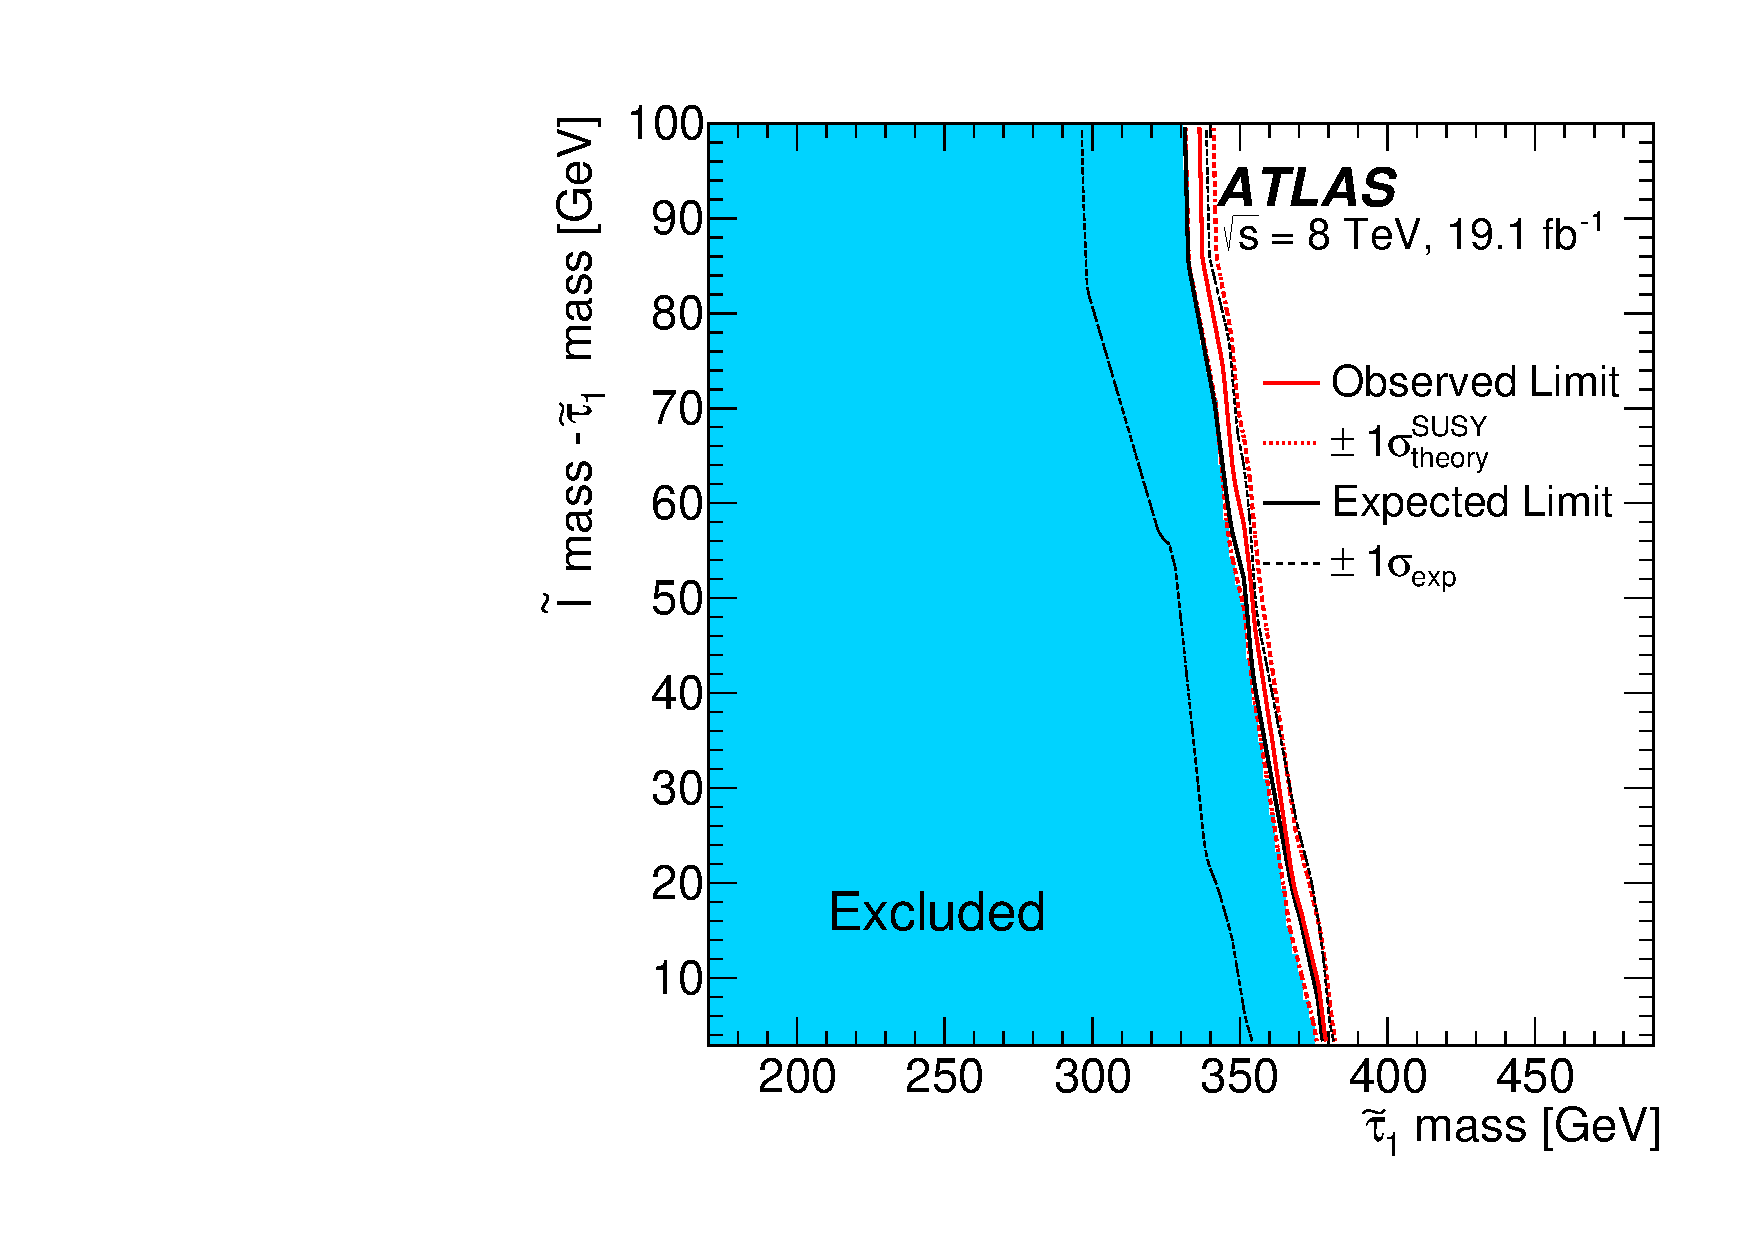
\includegraphics[width=\textwidth]{img/stau/fig_06a.pdf}
    \subcaption{}
    \end{minipage}
    \begin{minipage}{0.49\hsize}
    \centering   
    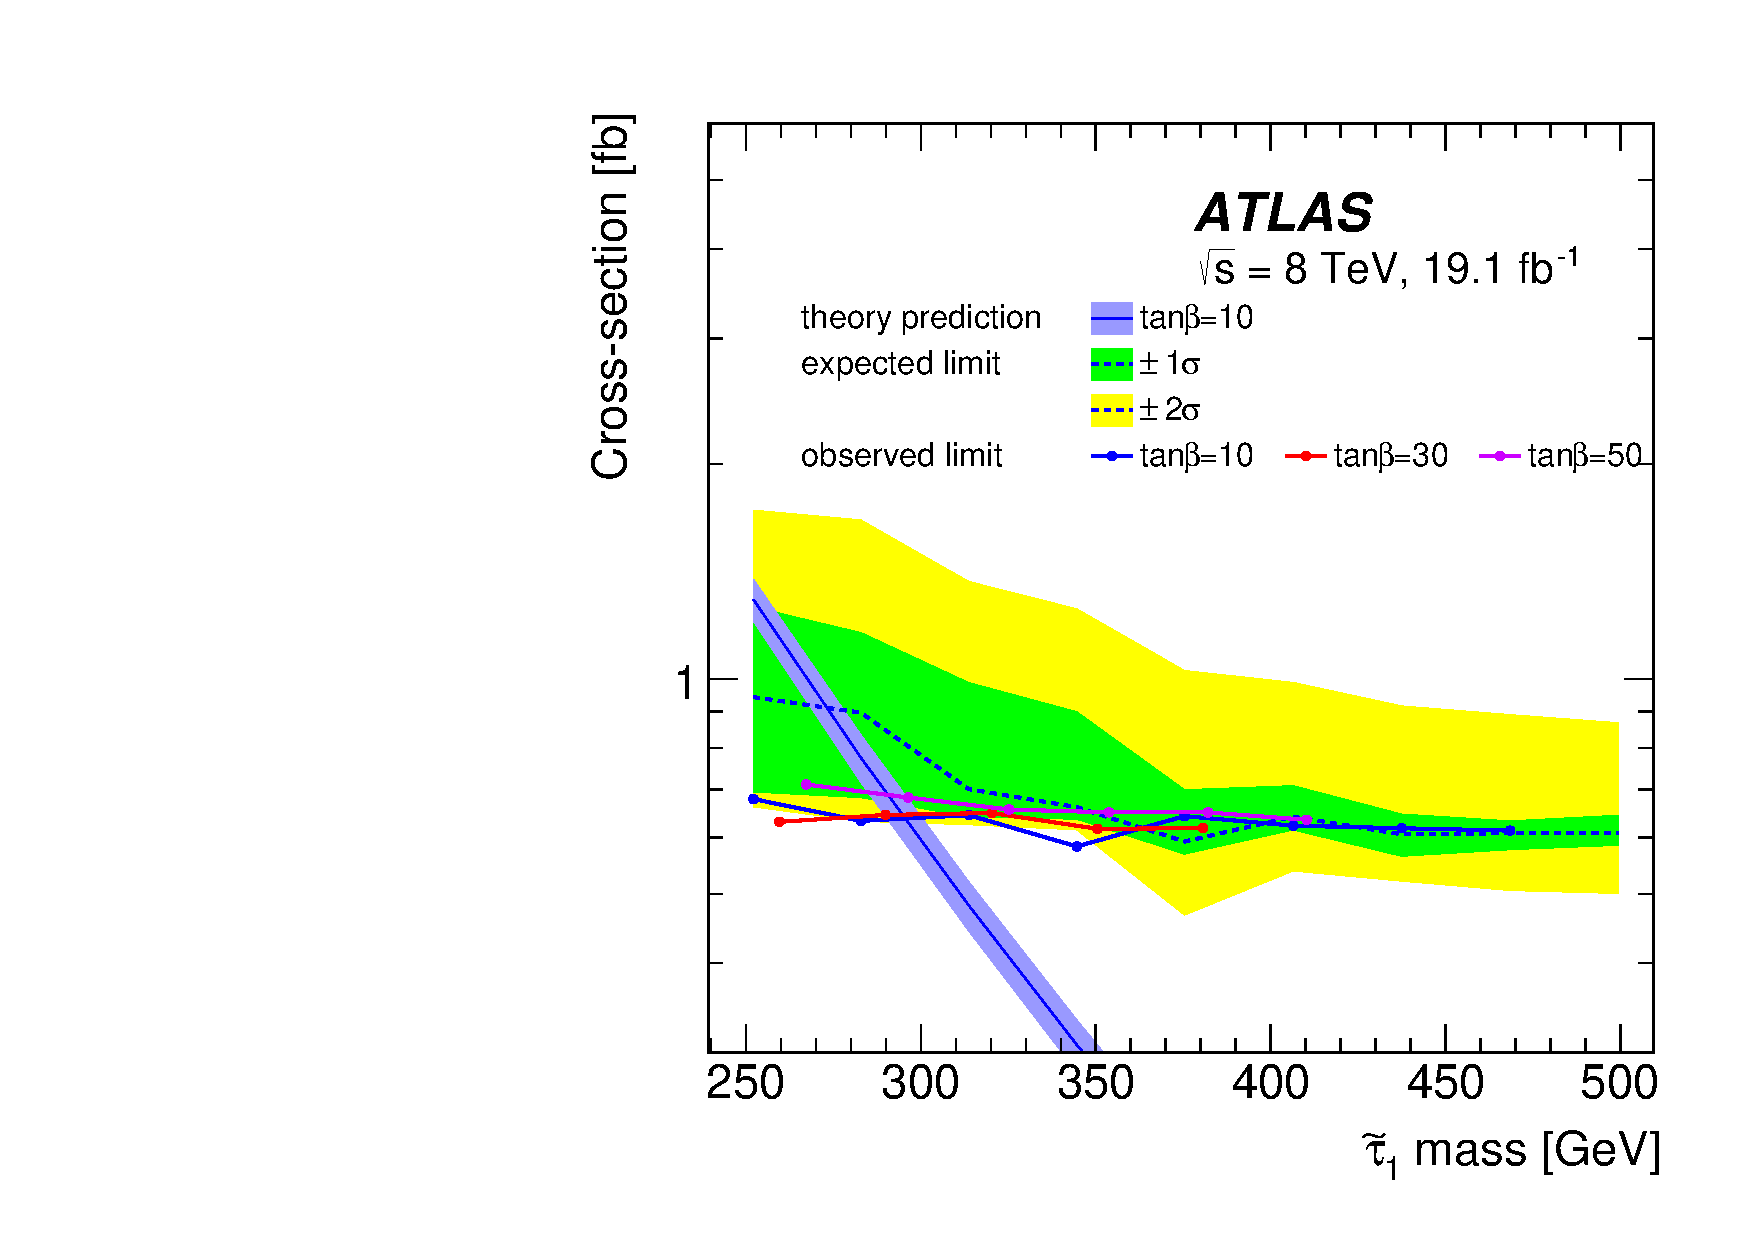
\includegraphics[width=0.99\textwidth]{img/stau/fig_07a.pdf}
    \text{(d)}
    \end{minipage}
    \caption[(a)~GMSB~スレプトン探索における観測データとシミュレーションにおける期待される~1~つの信号候補が再構成された質量$m_{\beta}$の分布。(b)~スレプトンで観測されたデータ、バックグラウンド推定値、および予想される信号。(c)~$95\%$信頼水準における直接生成されたスレプトンの除外領域。(d)~スタウ粒子を直接生成するための質量と$\rm{tan}\beta$の~3~つの値の関数としての断面積の上限。]{(a)~GMSB~スレプトン探索における観測データとシミュレーションにおける期待される~1~つの信号候補が再構成された質量$m_{\beta}$の分布~\cite{AR:03}。(b)~スレプトンで観測されたデータ、バックグラウンド推定値、および予想される信号~\cite{AR:03}~($\it{M}_{\tilde{\tau}}=\rm{345}~\rm{GeV},~\it{M}_{\tilde{\tau}}=\rm{437}~\rm{GeV}$の~2~つの候補信号領域)~。
    (c)~$95\%$信頼水準における直接生成されたスレプトンの除外領域~\cite{AR:03}。除外された領域は青色で表示されている。~予想される制限は黒い実線で描かれ、観測された制限は赤い実線で示されている。(d)~スタウ粒子を直接生成するための質量と$\rm{tan}\beta$の~3~つの値の関数としての断面積の上限~\cite{AR:03}。$\rm{tan}\beta=10$において予想される限界は、それぞれ$\pm1\sigma$と$\pm2\sigma$の不確実性バンドが緑と黄色で描かれている。$\rm{tan}\beta$の~3~つの値で観測された限界は、マーカー付きの実線で示されている。$\rm{tan}\beta=10$の理論的な断面積予測は、色付きの$\pm1\sigma$バンドとして示されている。}\label{fig:stau1}
\end{figure}

\section{スタウ粒子サンプル}
本論文では\subsecref{subsec:LSP}で述べた長寿命スタウ粒子の探索に焦点を当てて研究を行う。
スタウ粒子の特性を理解するためにシミュレーションサンプルを用いて各変数で想定される分布を算出した。\figref{fig:staud1}にスタウ粒子サンプルの$p_{\rm{T}},~\eta$方向における分布を示す。ミューオンは~105~MeV、スタウ粒子サンプルは~600~GeV,~1000~GeV~の質量でシミュレートされたサンプルを使用している。また\figref{fig:staud2}に各サンプルの粒子速度の分布を示す。粒子速度$\beta$は
\begin{align}
    \beta = \frac{v}{c} \label{eq:bb}
\end{align}
と表す。ここで、$v$は光速に対する粒子速度、$c$は光速度を表す。
スタウ粒子サンプルはミューオンに比べ、非常に質量が大きいため粒子速度の遅い領域まで分布が広がっていることが分かる。ミューオンに関しては、ほぼ光速$\left(\beta\simeq1\right)$の領域にしか存在していない。

\begin{figure}[tbp]
    \begin{minipage}{0.49\hsize}
    \centering   
    \includegraphics[width=\textwidth,page=2]{img/plot/beta.pdf}
    \subcaption{}
    \end{minipage}
    \begin{minipage}{0.49\hsize}
    \centering   
    \includegraphics[width=\textwidth,page=3]{img/plot/beta.pdf}
    \subcaption{}
    \end{minipage}
    \caption[スタウサンプルの$p_{\rm{T}},~\eta,$分布]{スタウサンプルの$p_{\rm{T}},~\eta,$分布。質量が~600~GeV,~1000~GeV~のサンプルを使用した。(a)$p_{\rm{T}}$分布。(b)$\eta$分布。}\label{fig:staud1}
\end{figure}

\begin{figure}[tbp]
    \begin{minipage}{0.49\hsize}
    \centering   
    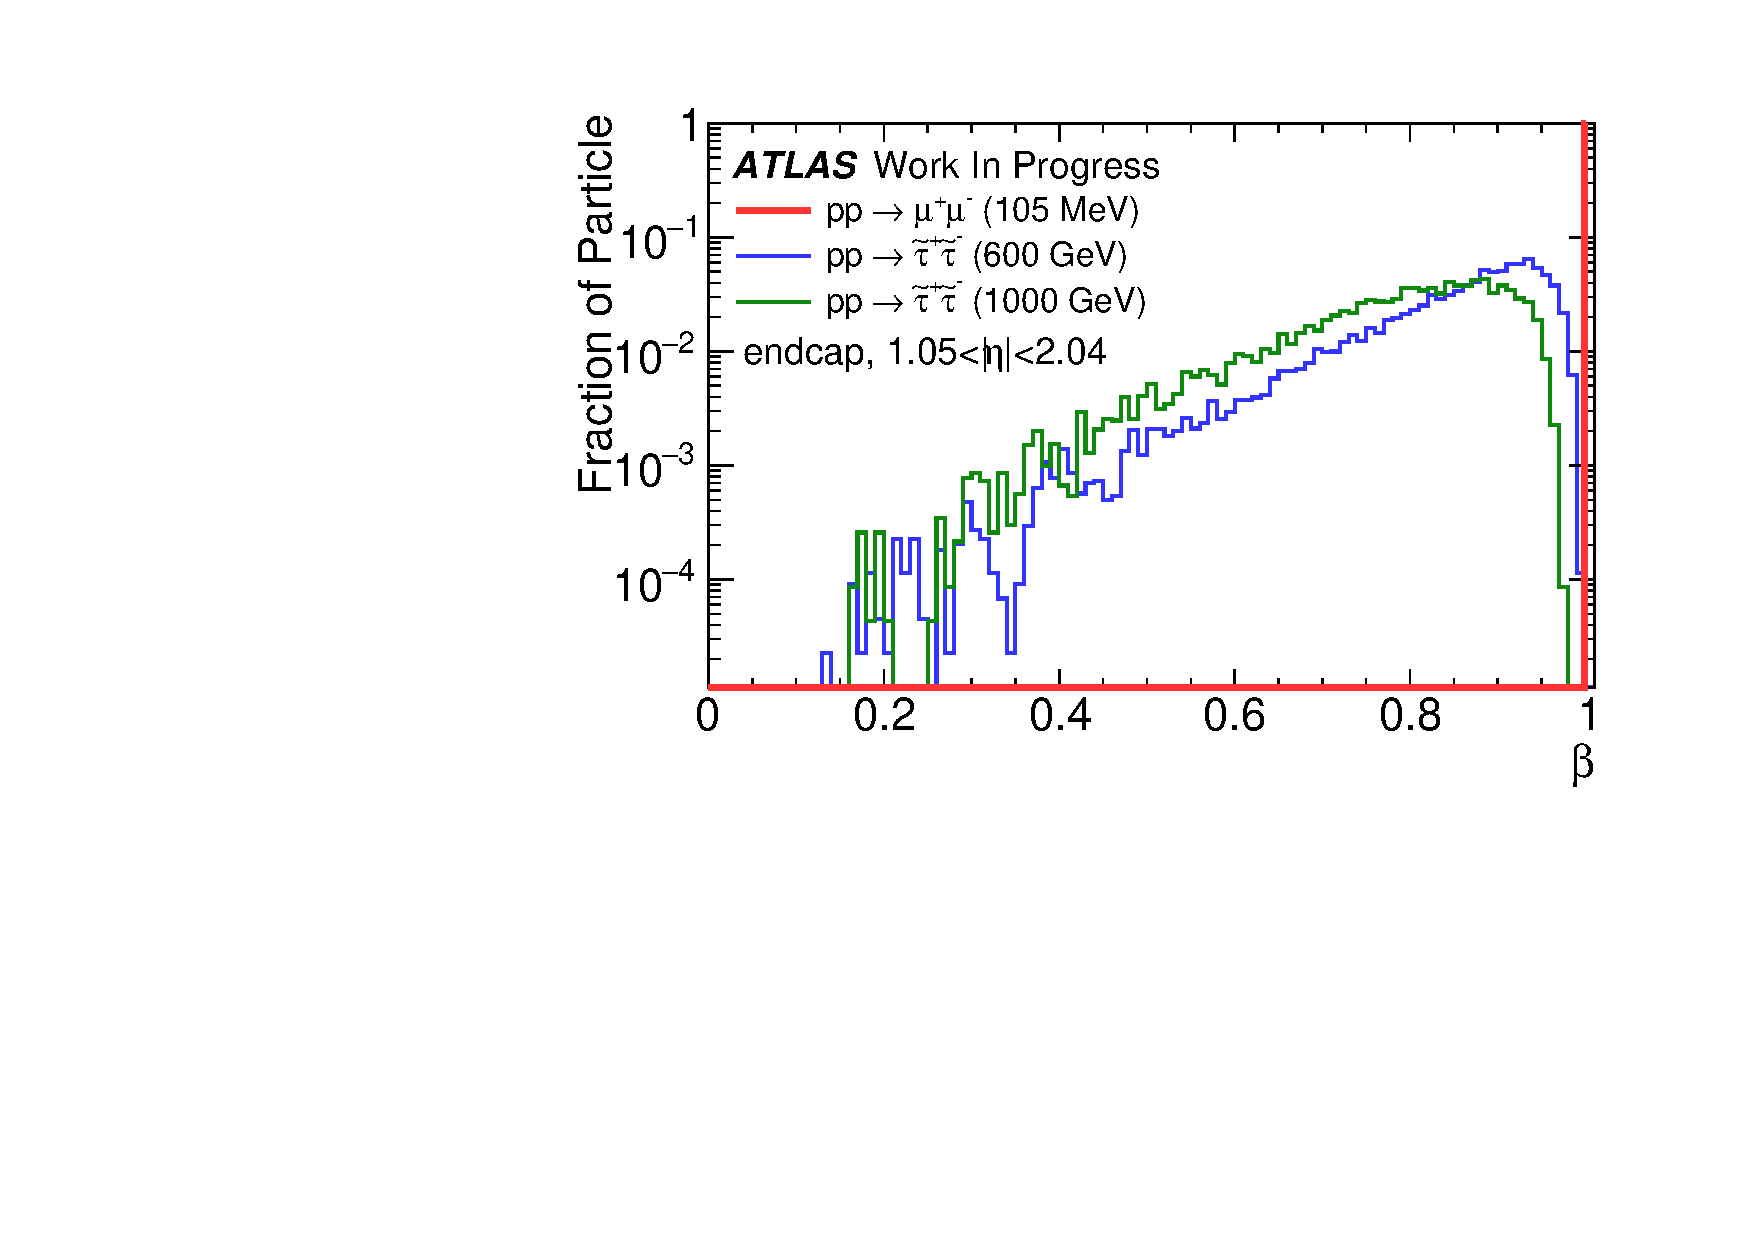
\includegraphics[width=\textwidth,page=1]{img/plot/beta.pdf}
    \subcaption{}
    \end{minipage}
    \begin{minipage}{0.49\hsize}
    \centering   
    \includegraphics[width=\textwidth,page=5]{img/plot/beta.pdf}
    \subcaption{}
    \end{minipage}
    \caption[スタウサンプルとミューオンサンプルにおける粒子速度分布]{スタウサンプルとミューオンサンプルにおける粒子速度分布。ミューオンは質量が~105~MeV,~スタウサンプルは質量が~600~GeV,~1000~GeV~である。(a)~はエンドキャップ領域、(b)~はバレル領域の分布を示す。}\label{fig:staud2}
\end{figure}

\section{シングルミューオントリガー}
\label{sec:single}
本研究で対象としている長寿命スタウ粒子は、寿命が長く安定しているため~ATLAS~検出器の最外に位置するミューオン検出器まで到達すると考えられている。また荷電粒子であるためミューオン検出器での直接検出が可能である。そのため~ATLAS~実験~Run~2~においては標準的なシングルミューオントリガーが解析に用いられていた。\figref{fig:sumi1}は、シングルミューオントリガーにおけるスタウ粒子の取得効率を示している。この図を見ると、スタウ粒子の質量が増加するに従って取得効率が低下していることが確認できる。
$p_{\rm{T}}$閾値~20~GeV~のトリガーの場合、トリガー効率はエンドキャップ領域で約$85\%$であることが知られている。しかし、スタウ粒子のサンプルにおいては$p_{\rm{T}}$が高いにもかかわらず、質量が増加するとトリガー効率が低下し、911~GeV~では約$50\%$に低下している。

\secref{sec:ttri}で述べたようにミューオントリガーは、大きく分けて~L1~と~HLT~の~2~つに分かれている。本節では、それぞれのトリガーの速度の遅い荷電粒子に対する事象選別の特徴と問題点について述べる。

\begin{figure}[tbp]
        \centering   
        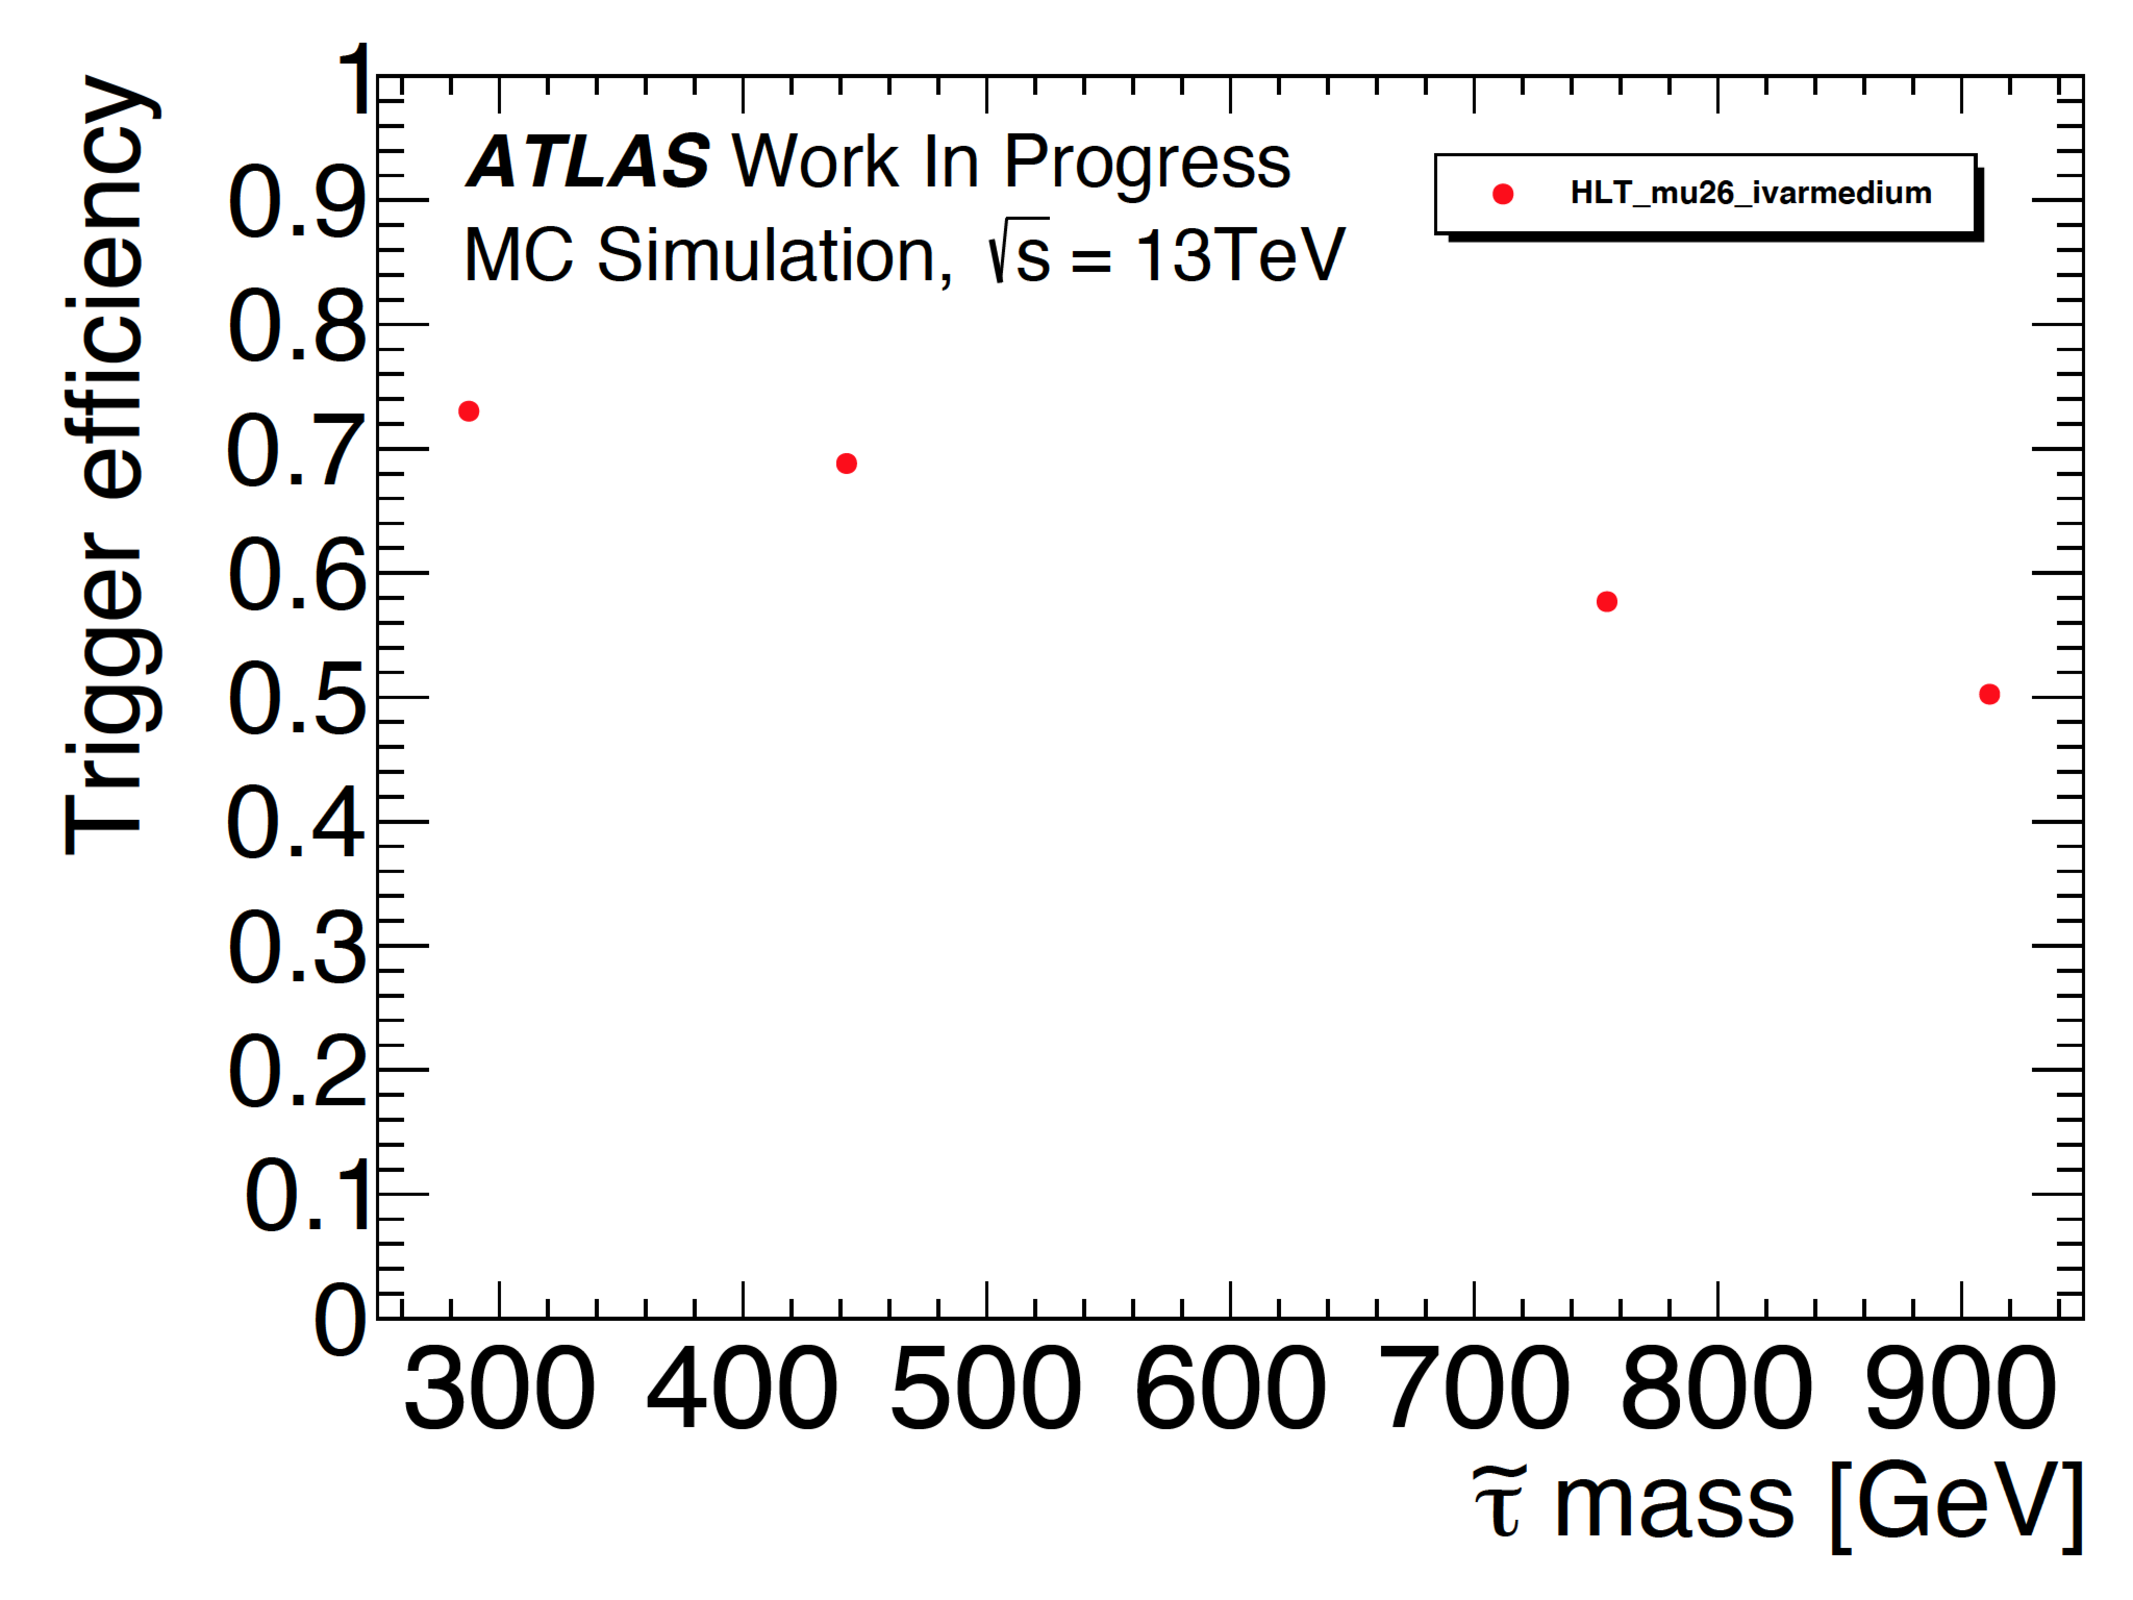
\includegraphics[width=0.7\textwidth,page=1]{img/pdf3/sumi.pdf}
        \caption[シングルミューオントリガーによるスタウ粒子の質量に依存した取得効率]{シングルミューオントリガーによるスタウ粒子の質量に依存した取得効率~\cite{MT:01}。}
        \label{fig:sumi1}
\end{figure}

\subsection{L1~シングルミューオントリガー}
SM~粒子と比べはるかに質量が大きいスタウ粒子では、シングルミューオントリガーにおける取得効率は低下する。これはスタウ粒子の速度が、ほぼ光速の~SM~粒子に比べ、小さいことに由来する。\figref{fig:sumi2}にシングルミューオントリガーによるスタウ粒子の速度に依存した取得効率を示した。標準的なシングルミューオントリガーにおいては$\beta>0.8$の領域にしか感度がないことが分かる。
\secref{sec:ttri}で述べたように~Run~2~のトリガーシステムでは、基本的に粒子が光速で検出器に到達することを仮定している。Run~2~の初期においては、遅い粒子の情報を取得する必要性が認識されておらず、光速の粒子のトリガーを行うことに焦点が当てられていた。したがって、速度の遅い粒子を標準的なシングルミューオントリガーのみでとらえるには限界があり、重い長寿命荷電粒子の探索は標準的なシングルミューオントリガーのみでは不十分であると言える。
\begin{figure}[tbp]
        \centering   
        \includegraphics[width=0.7\textwidth,page=2]{img/pdf3/sumi.pdf}
        \caption[シングルミューオントリガーによるスタウ粒子の速度に依存した取得効率]{シングルミューオントリガーによるスタウ粒子の速度に依存した取得効率~\cite{MT:01}。$\beta_{\Tilde{\tau}}^{\rm{true}}$はスタウ粒子の粒子速度を表す。}
        \label{fig:sumi2}
\end{figure}

\subsection{HLT~ミューオントリガー}
HLT~ミューオントリガーにおいては、飛跡の再構成のために~MDT~検出器を用いている。MDT~検出器では、荷電粒子が通過することによって電離された電子がセンサーに信号として読みだされるまでのドリフト時間を計算する。
ドリフト速度は一定であるため、ドリフト時間からドリフト半径を求めることができる。実際に荷電粒子が~MDT~検出器を通過する様子を示したものが\figref{fig:mdt}である。複数の~MDT~検出器からドリフト半径を求め、半径の接線を結ぶことにより飛跡の再構成を行う。

粒子の速度が遅い場合、上記の飛跡再構成手法には問題点が存在する。通常のアルゴリズムでは粒子の飛行時間を求める際に、粒子速度が光速であることを仮定して計算が行われている。従って速度の遅い粒子では、飛行時間が長くなるためドリフト半径を誤って本来よりも大きい値として計算してしまう。以上の影響により遅い荷電粒子に対して、誤った飛跡再構成が行われる。
そこで、HLT~の遅い荷電粒子用トリガーにおいては飛行時間が誤っていることを想定し、飛行時間を変化させながら再構成を行うという手法をとる。内部飛跡検出器から外挿された飛跡とのマッチングをとることで飛跡を一意に決定する。
\figref{fig:hlt}に~HLT~におけるトリガー効率を示した。トリガー効率には粒子速度による依存性は見られず、約$80\%$のトリガー効率を達成している。しかし、光速のミューオンに対する~HLT~のトリガー効率は約$90\%$であることが知られている。これは一部の領域においてドリフト時間を変化させるフィッティングによって一意に飛跡を決定できないことが原因である。この問題を解消する方法として、あらかじめ数種類のドリフト時間を仮定し、飛跡候補の選択肢を用意しておく手法が提案されたが、処理時間増加の観点から~Run~3~での導入は難しいと考えられている~\cite{MT:01}。

\begin{figure}[tbp]
        \centering   
        \includegraphics[width=0.65\textwidth,page=2]{img/pdf3/mdt.png}
        \caption[ミューオンが通過した際の飛跡再構成の様子]{ミューオンが通過した際の飛跡再構成の様子~\cite{MT:01}。各~MDT~ヒットに対するドリフト半径を結んだ接線を求めることで飛跡の再構成を行う。}
        \label{fig:mdt}
\end{figure}

\begin{figure}[tbp]
        \centering   
        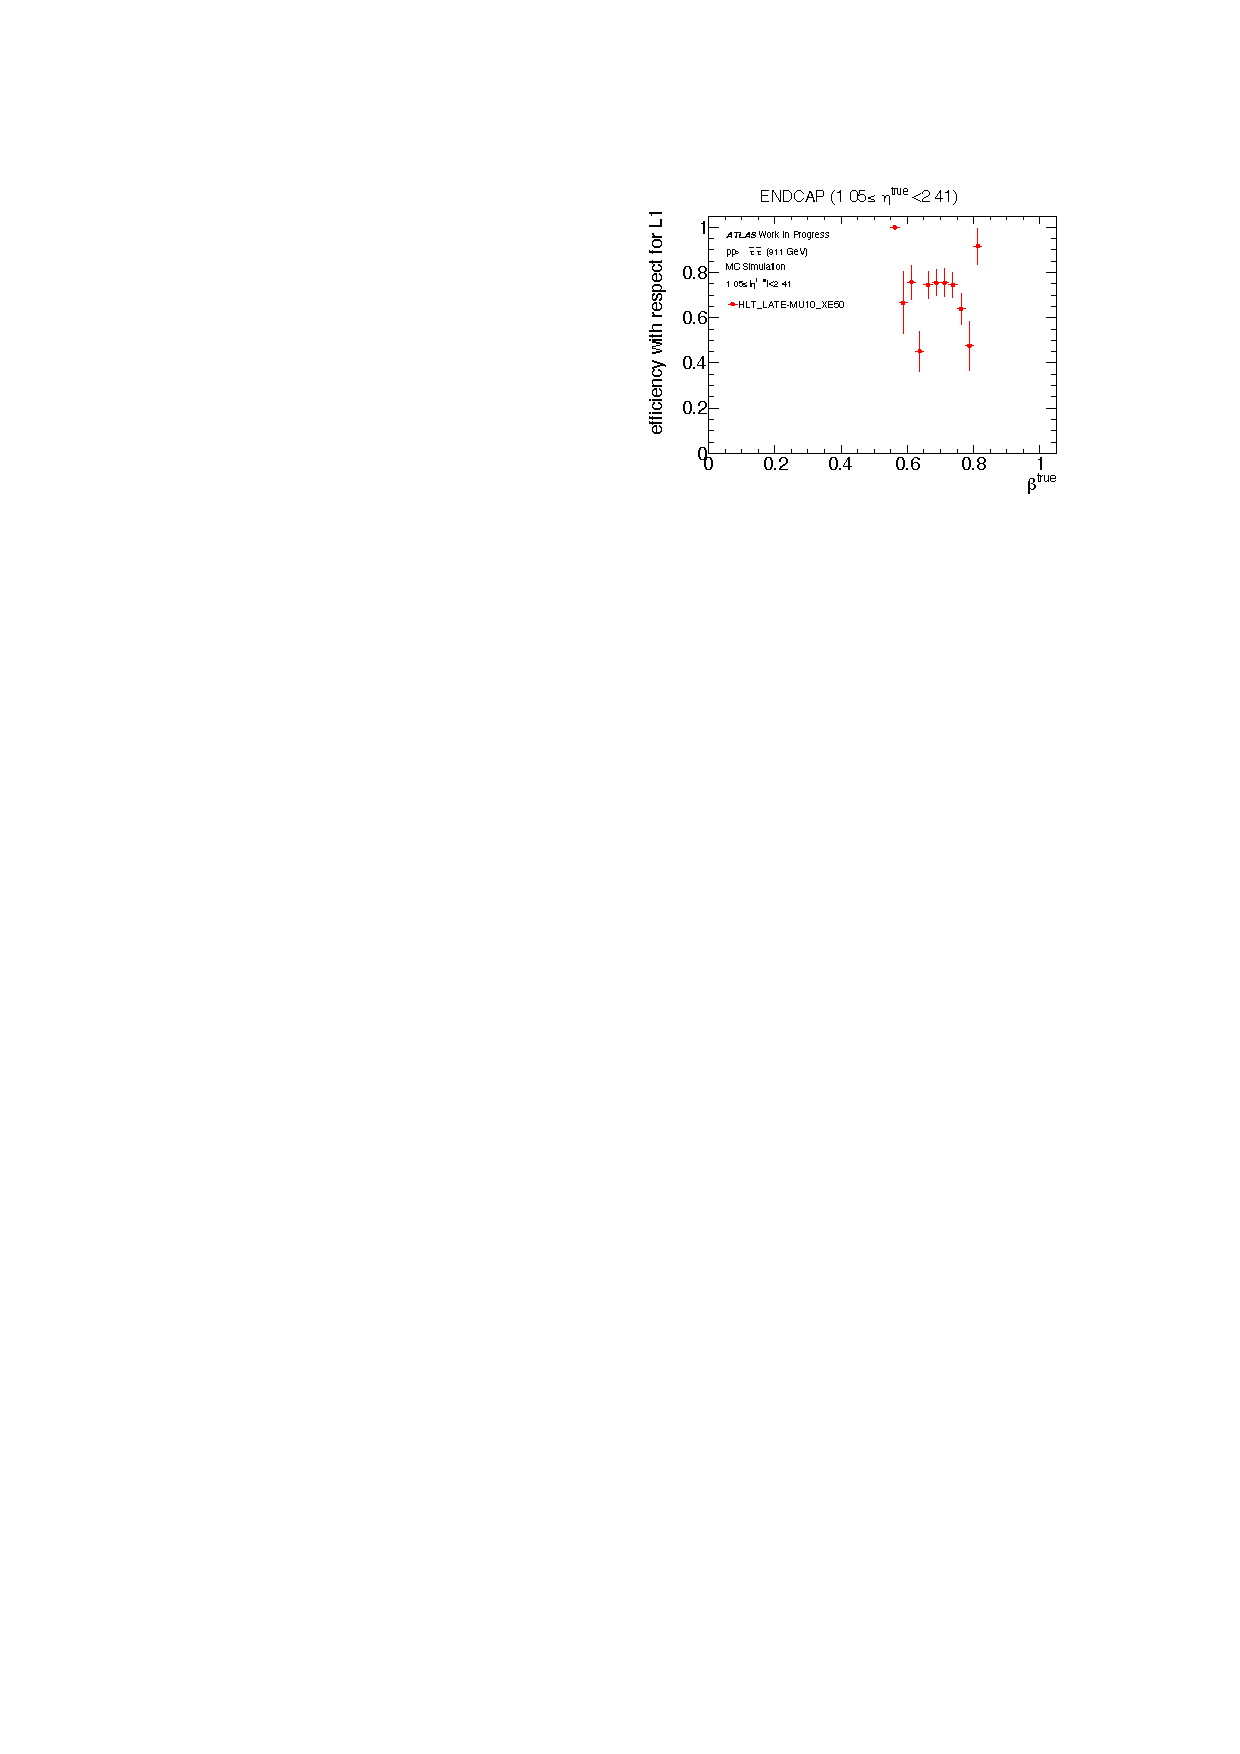
\includegraphics[width=0.75\textwidth,page=1]{img/pdf3/hlt.pdf}
        \caption[エンドキャップ領域における速度に依存した HLT のトリガー効率]{エンドキャップ領域における速度に依存した~HLT~のトリガー効率~\cite{MT:01}。$\beta_{\Tilde{\tau}}^{\rm{true}}$はスタウ粒子の粒子速度を表す。}
        \label{fig:hlt}
\end{figure}

\section{遅い荷電粒子探索用~L1~トリガー}
\label{sec:latemu}
標準的なシングルミューオントリガーでは$\beta<0.8$の領域にしか感度がなかった。これはL1~シングルミューオントリガーが、基準バンチの情報のみをトリガー判定に利用していたことによるものである。ATLAS~実験においても、速度の遅い荷電粒子探索の必要性が認識され、新たな~L1~の遅い荷電粒子探索用トリガーが~Run~2~の後半に試験的に導入された。このトリガーは速度が遅い粒子の情報を取得するために、基準バンチの次のバンチのタイミングでミューオン検出器に到達した粒子に感度を持つ。しかし、ミューオントリガーのみでトリガー判定を行うと、次バンチであることの保証ができない。実験においては次バンチであることの保証のために、別の検出器で基準バンチのタイミングを要求する。遅い荷電粒子探索用トリガーにおいては、カロリメータで基準バンチに~MET~またはジェットが存在することを要求することでタイミングの保証をしている。\figref{fig:met}に要求する事象のイメージ図を示す。

\figref{fig:sumi3}は、スタウ粒子のシングルミューオントリガー、遅い荷電粒子探索用トリガーおよび~MET~トリガーの速度に依存した取得効率を示している。
遅い荷電粒子探索用トリガーは$0.6 < \beta < 0.8$の領域に感度があることが分かる。
トリガー効率が約$30\%$であるのは~MET~トリガーの効率が$30\%$程であることによる。

\begin{figure}[tbp]
        \centering   
        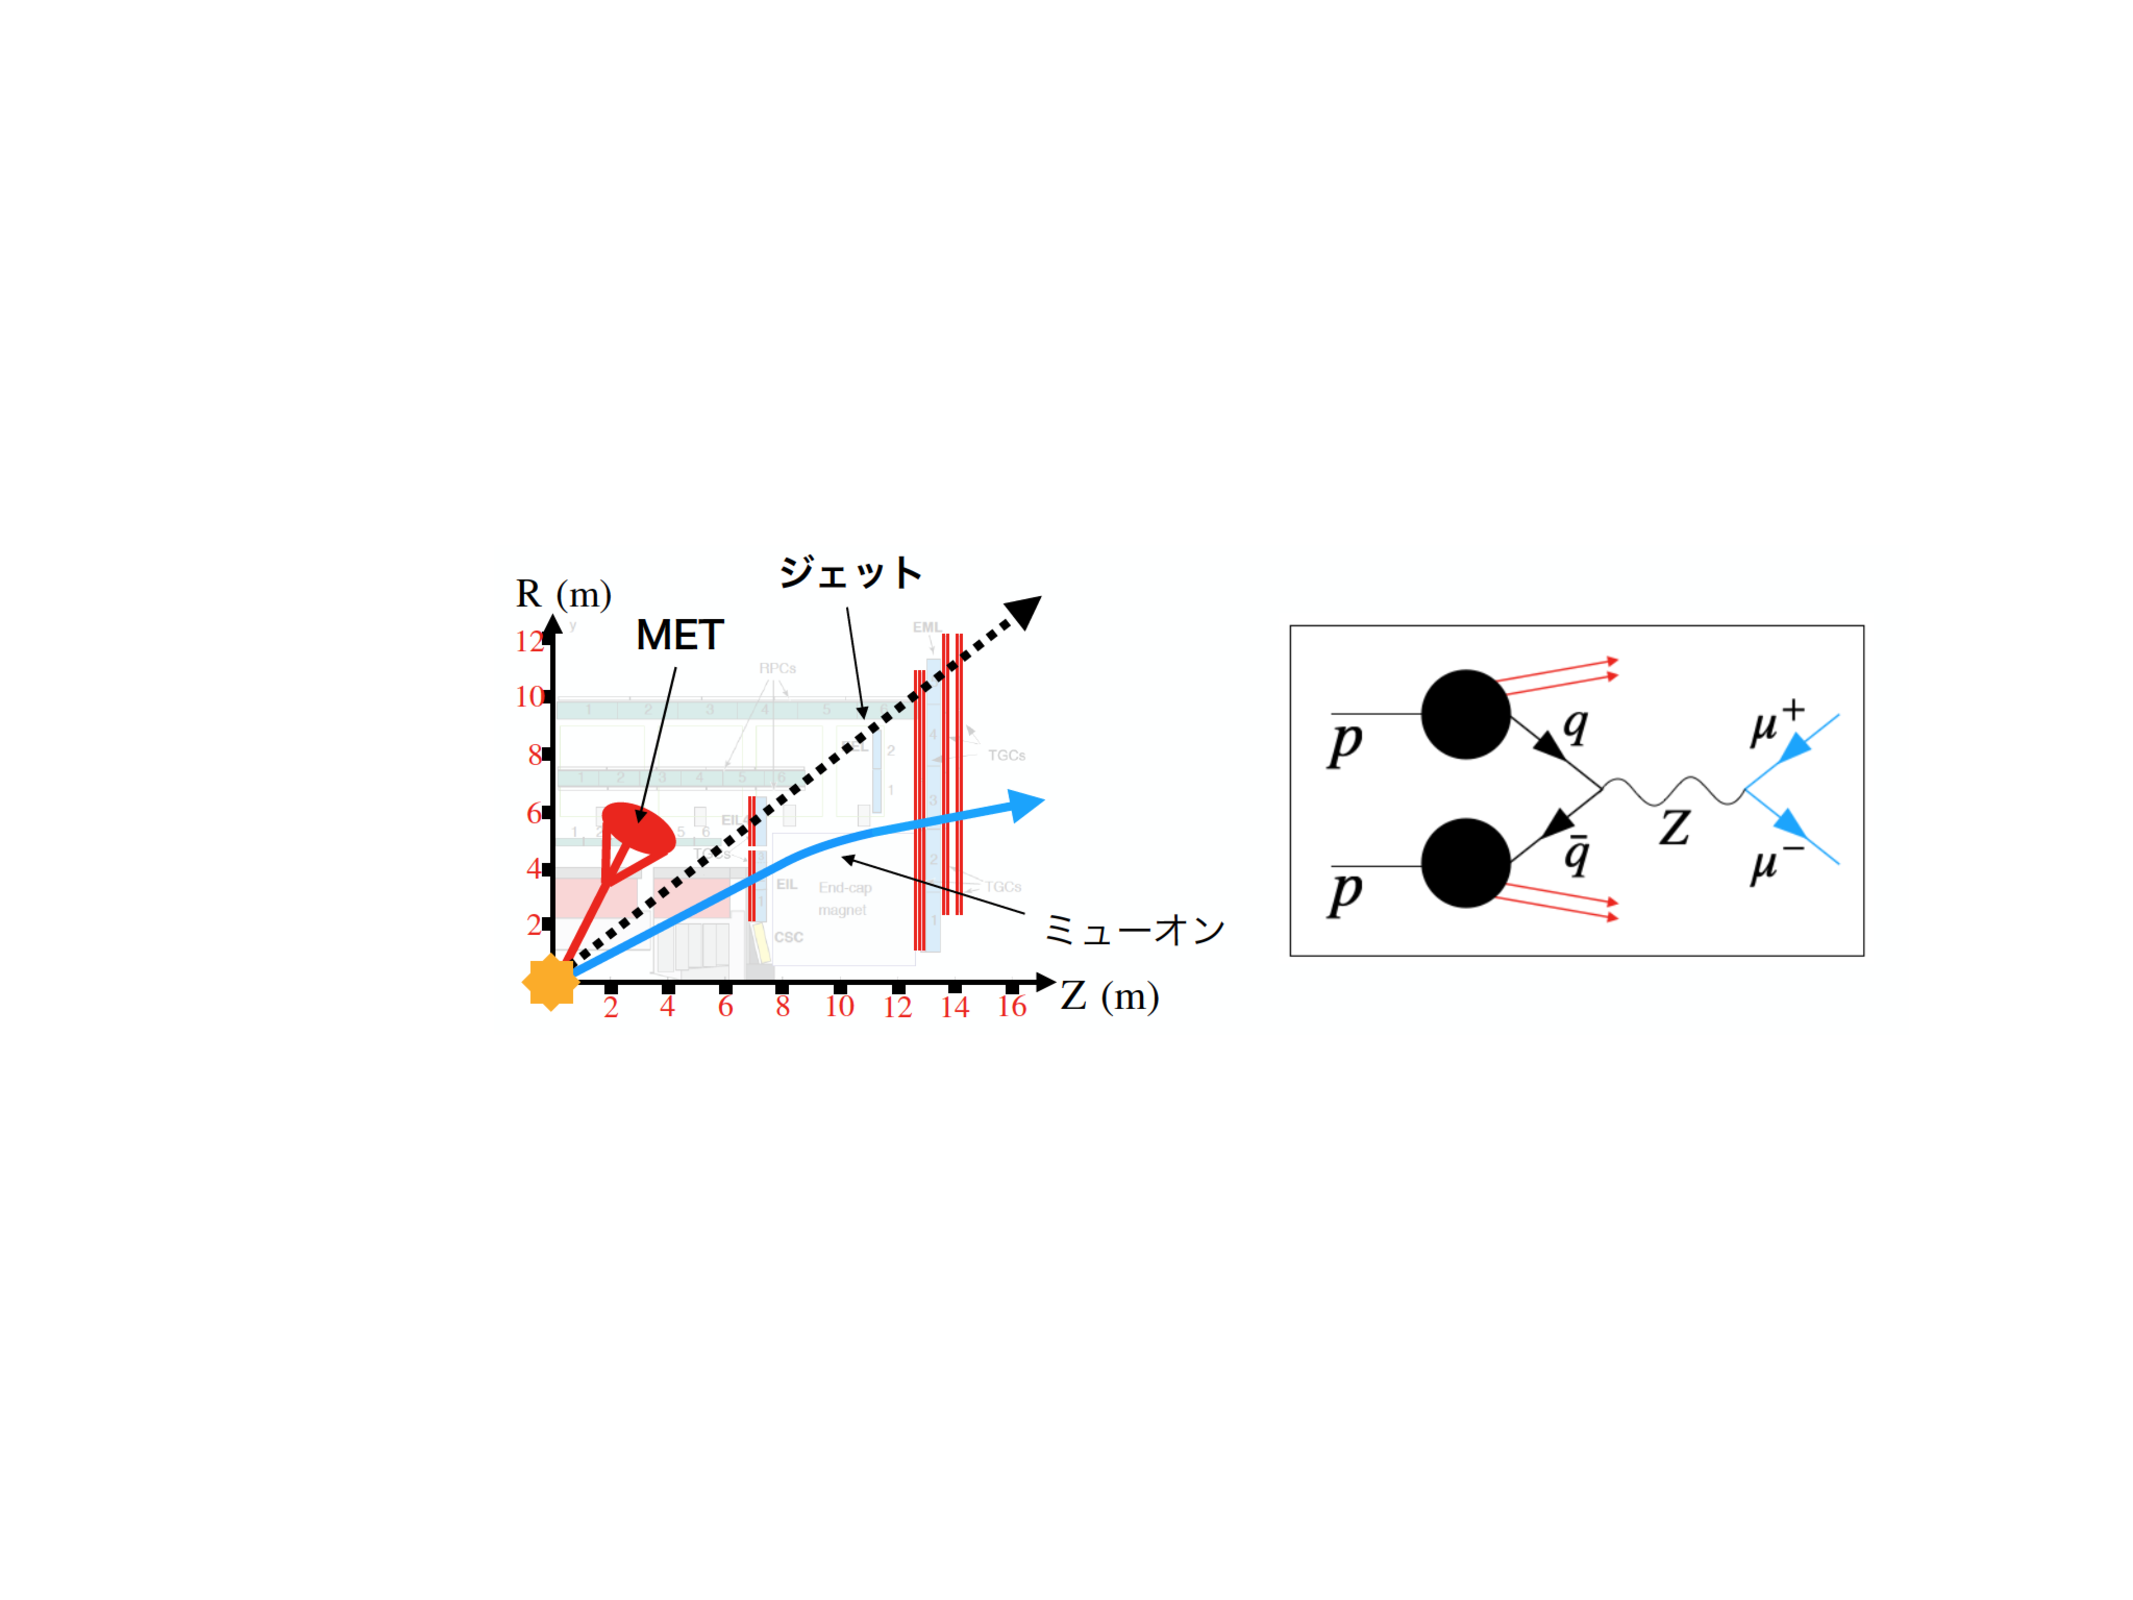
\includegraphics[width=\textwidth,page=1]{img/pdf3/met.pdf}
        \caption[遅い荷電粒子探索用トリガーが要求する事象のイメージ図]{遅い荷電粒子探索用トリガーが要求する事象のイメージ図。左図は遅い荷電粒子探索用トリガーが要求する事象の様子を示している。右図は想定される崩壊過程を示しており、赤が~MET~またはジェット、青がミューオン等の荷電粒子を示す。MET~またはジェットを基準バンチに要求し、ミューオン等の荷電粒子を次バンチに要求する。}
        \label{fig:met}
\end{figure}

\begin{figure}[tbp]
        \centering   
        \includegraphics[width=0.7\textwidth,page=3]{img/pdf3/sumi.pdf}
        \caption[スタウ粒子の速度に依存した取得効率]{スタウ粒子の速度に依存した取得効率~\cite{MT:01}。赤色、青色、緑色はそれぞれシングルミューオントリガー、遅い荷電粒子探索用トリガー、MET トリガーを示している。$\beta_{\Tilde{\tau}}^{\rm{true}}$はスタウ粒子の粒子速度を表す。}
        \label{fig:sumi3}
\end{figure}

\section{本研究の目的}
\secref{sec:single}、\secref{sec:latemu}より標準的なミューオントリガーと遅い荷電粒子探索用トリガーを組み合わせれば、
$0.6 < \beta < 1.0$の領域に感度を持つことが分かった。
\figref{fig:sumi4}は、スタウ粒子のシングルミューオントリガーおよび遅い荷電粒子探索用トリガーの速度に依存した取得効率を示している。遅い荷電粒子探索用トリガーには~MET~の要求をしていない。
緑色で示された両者の論理和を見ると$\beta\sim0.8$の領域において効率が少し低下していることが分かる。このようなことが起こる一つの原因として、ミューオン検出器の各層でのタイミング判定にずれがあることが考えられる。ミューオン検出器のある層では基準バンチ、他の層では次バンチと判定された場合、両者のトリガーを通過してしまう可能性がある。

\figref{fig:time}に示すような~TGC~の~M1~から~M3~における粒子到来の時間差$t_{\rm{M13}}$は、粒子の速度によって異なる。
例えば$|\eta|=1.4$の場合、$\beta=1.0$で$t_{\rm M13}\simeq6.7~\rm ns$、$\beta=0.8$で$t_{\rm M13}\simeq8.4~\rm ns$、$\beta=0.6$で$t_{\rm M13}\simeq11.2~\rm ns$と計算され
$t_{\rm{M13}}$が大きいほどバンチ判定による一致が取れない確率が高くなるためトリガー効率の低下が懸念される。
以上の影響を最小限にしトリガー効率を向上させるためには、各チェンバーにおいて判定される粒子信号のタイミング判定をナノ秒単位でより詳細に行う必要がある。
ミューオン検出器におけるタイミング判定は、効率的に粒子情報を取得する上で非常に重要な要素の一つと言える。
\begin{figure}[tbp]
        \centering   
        \includegraphics[width=0.7\textwidth,page=4]{img/pdf3/sumi.pdf}
        \caption[スタウ粒子の速度に依存した取得効率]{スタウ粒子の速度に依存した取得効率~\cite{MT:01}。赤色、青色、緑色はそれぞれシングルミューオントリガー、遅い荷電粒子探索用トリガー~(MET~の要求なし)、両トリガー論理和を示している。$\beta_{\Tilde{\tau}}^{\rm{true}}$はスタウ粒子の粒子速度を表す。}
        \label{fig:sumi4}
\end{figure}
\begin{figure}[tbp]
        \centering   
        \includegraphics[width=0.4\textwidth,page=4]{img/pdf3/time.png}
        \caption[M1~から~M3~までにかかる粒子到来時間差$t_{\rm M_{13}}$の概念図]
        {M1~から~M3~までにかかる粒子到来時間差$t_{\rm M_{13}}$の概念図。}
        \label{fig:time}
\end{figure}

本研究では、ミューオン検出器の一つである~TGC~検出器に着目し、タイミング判定における詳細な見積もりおよび検証を行う。そして~TGC~検出器のタイミング調整に伴ったトリガー効率について調査し、TGC~の性能改善を目指す。光速のミューオンおよび遅い荷電粒子に対するトリガー効率の評価を行い、Run~3~に向けた感度向上に取り組む。

解析には~Run~2~における実験データおよびモンテカルロシミュレーションを用い、両者の比較、検証を行うことで問題点並びに改良点を示唆する。
Run~3~では、より詳細な新物理探索を目指す上で~Run~2~以上に精密な処理が要求される。TGC~検出器のタイミング較正により、Run~3~に向けた~TGC~検出器の最適な実装を提案する。

\chapter{TGC~システム}
\thispagestyle{empty}
\label{chap:4}
TGC~検出器~\cite{TR:04}は~MWPC~であり、ワイヤーとストリップが互いに交差して配置されているため二次元読み出しを可能にしたトリガー用前後方ミューオン検出器である。本章では~TGC~検出器の詳細および信号読み出しのための各エレクトロニクスについて記す。
\section{TGC~の動作原理}
TGC~は、動作ガスとして$\rm{CO_2}$/n-Pentane~(55:45)~を使用している。ワイヤーには通常~2.8~keV~の高電圧が印加されている。ガス中を荷電粒子が通過すると、その経路にあるガス分子が電離される。電離された一次電子は陽極側にドリフトしながら印加電場によって加速され、ガス分子の電離エネルギーを超えると二次電子を生成する。以上のような電子生成を繰り返すことでカスケード型の電子雪崩を生成する。電子とイオン雲はそれぞれドリフトによって互いに離れ、電子雲はワイヤーを取り囲み、イオン雲はさらに周りを取り囲むようにワイヤーの半径方向に拡散してゆく。TGC~検出器は以上の過程でできた電子雪崩をシグナルとしてワイヤーから読み取る。同時にカソード面では、塗布された高抵抗のカーボン面に電荷が誘起され、外側のストリップにも同様に電荷が誘起されることで信号として読み出される。

アノードワイヤーには直径$50~\mu\rm{m}$の金メッキタングステンを使用しており、ワイヤー間隔を~1.8~mm~と小さく設計することで時間応答を向上させている。カソードにはエポキシガラス板の片面に$\rm{1}~\rm{M}\Omega/\rm{cm}^2$のカーボンを
塗布したものを使用している。エポキシガラスの反対側には、銅のストリップがワイヤーと直行するように配置されている。ストリップ間隔は、$15\sim53~mm$で構成されている。ガスギャップおよびワイヤー間隔が小さいことで検出器の時間応答性を向上させている。

また電子雪崩によって生じた励起分子やイオン再結合により発生する紫外線は、カソード面やガスに衝突して発生する二次電子によって放電を起こす可能性がある。したがって紫外線を吸収する効果~(クエンチ効果)~のある~n-Pentane~を封入している。
\figref{fig:tgc2d}に~TGC~の信号読み出しの概念図、\figref{fig:TGCpri}に~TGC~検出器の詳細な構成を示した。

\begin{figure}[H]
        \centering   
        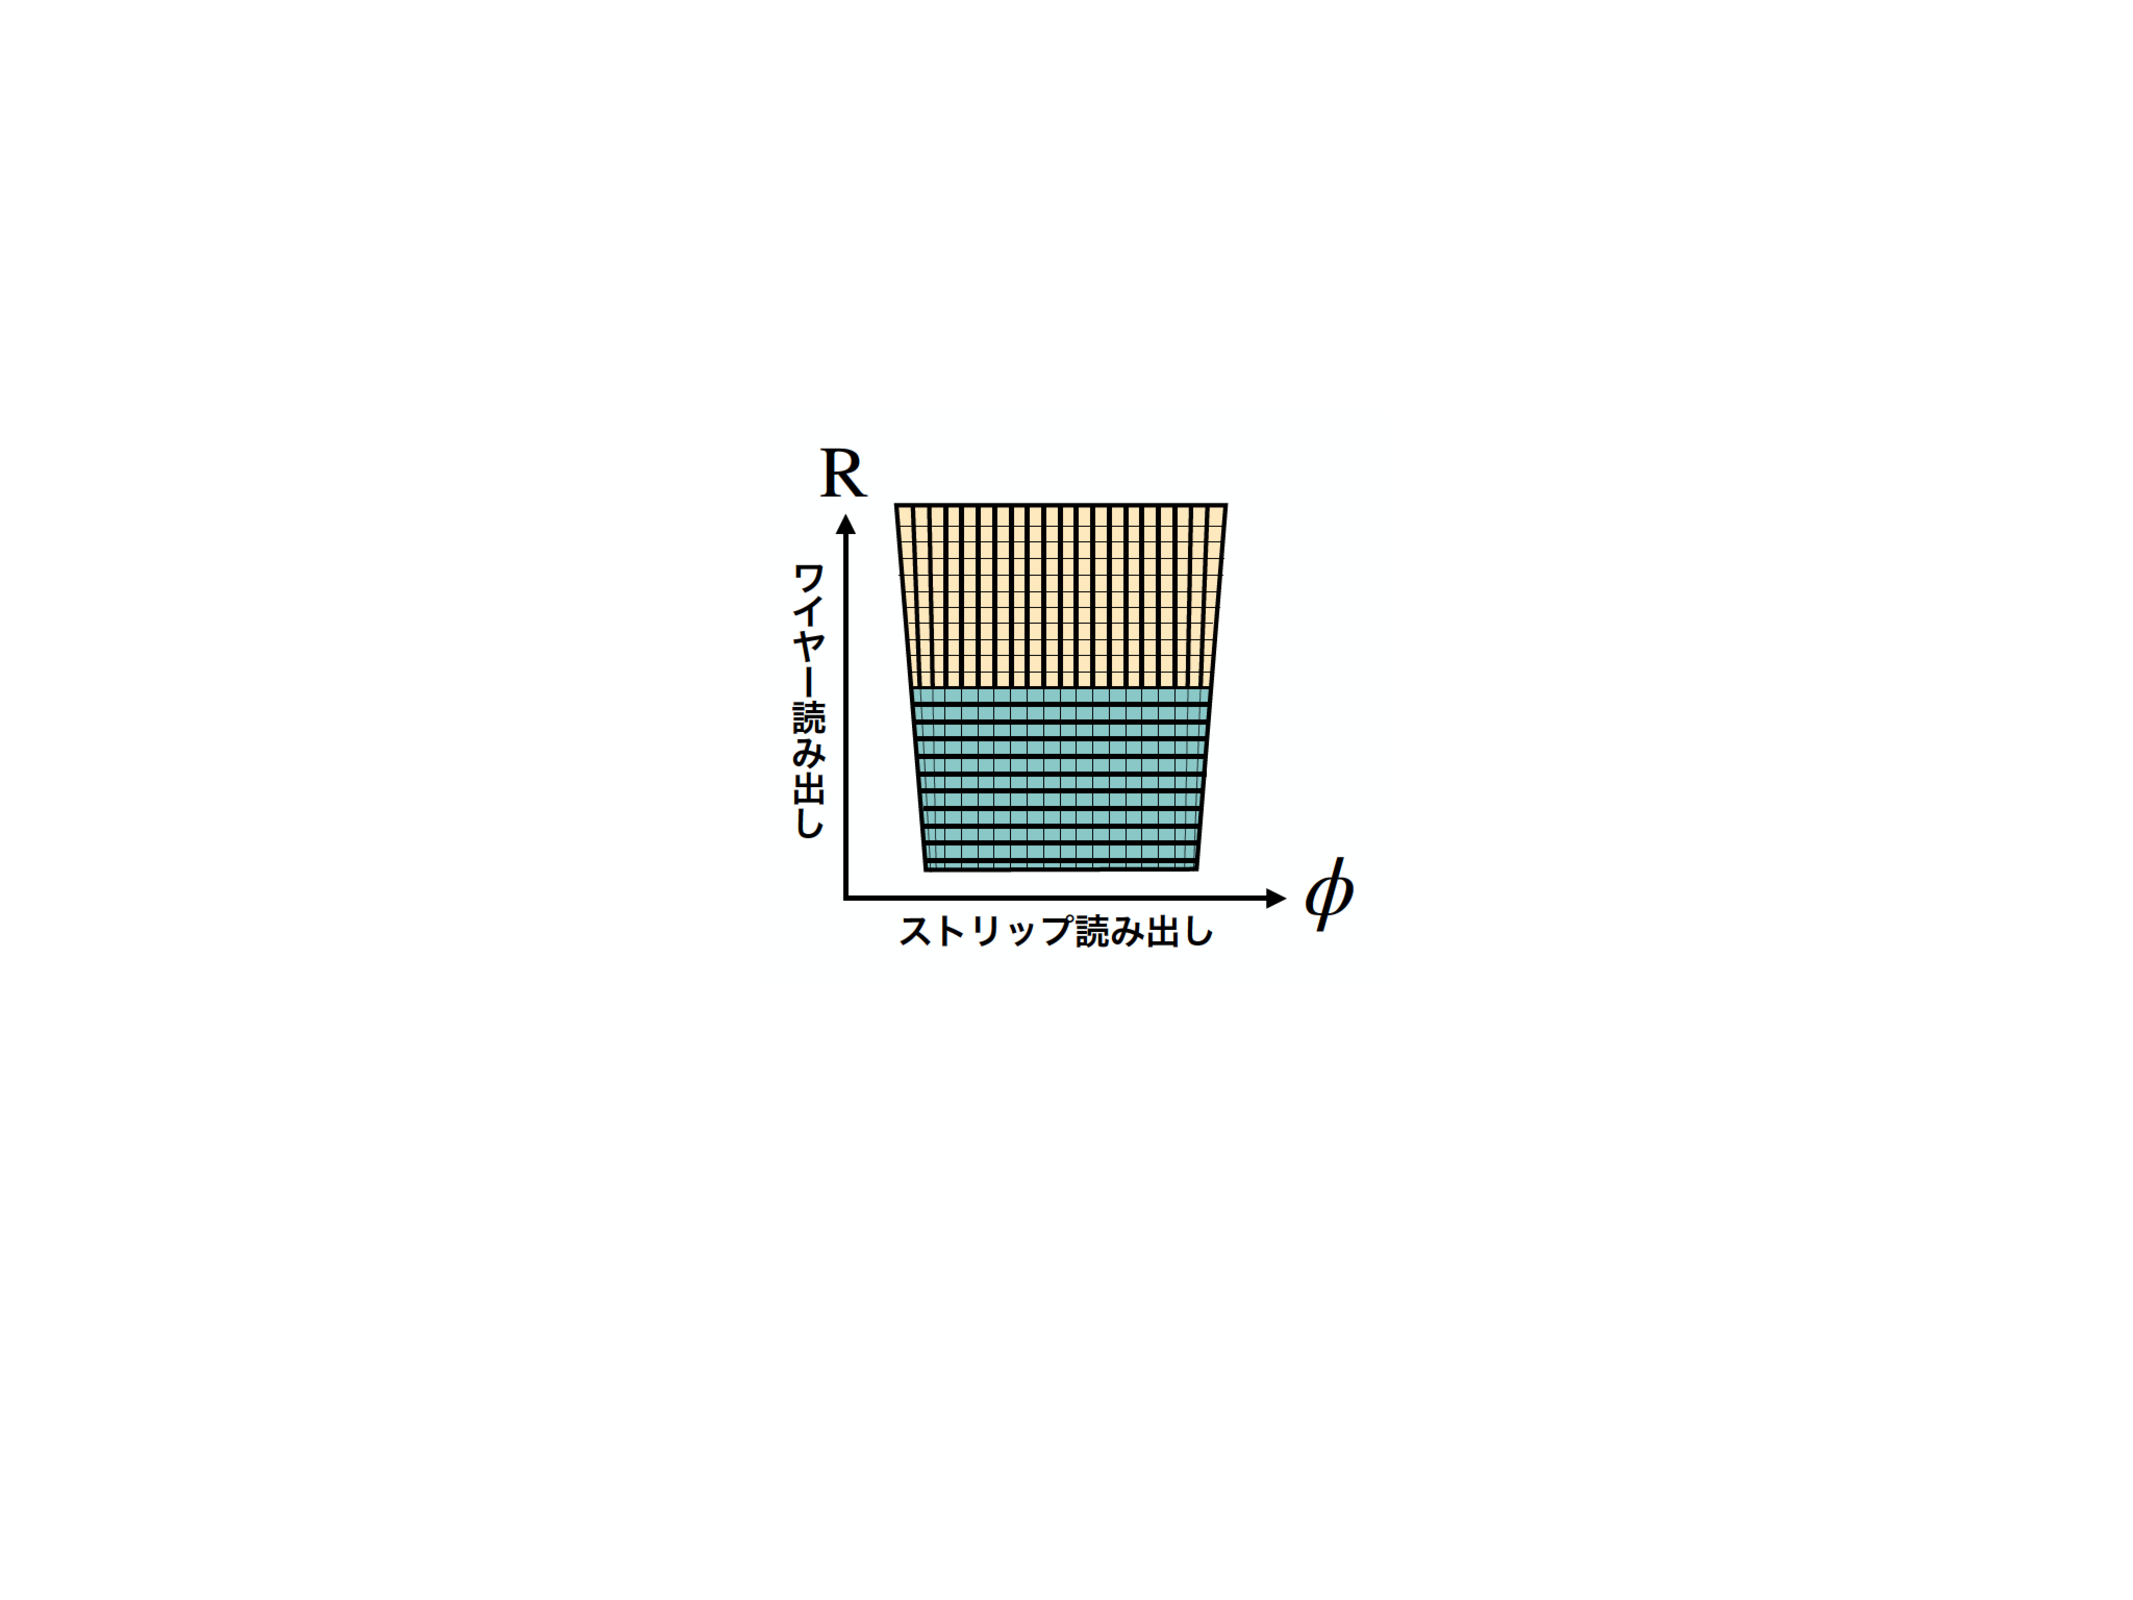
\includegraphics[width=0.6\textwidth,page=1]{img/pdf/tgc2d.pdf}
        \caption[TGC~二次元信号読み出しの概念図]{TGC~二次元信号読み出しの概念図。ワイヤーで$R$方向を測定し、ストリップで$\phi$方向を測定する。}\label{fig:tgc2d}
\end{figure}

\begin{figure}[H]
        \centering   
        \includegraphics[width=\textwidth,page=10]{img/pdf/ATLAS.pdf}
        \caption[TGC~検出器の~triplet~および~doublet~における断面図]{TGC~検出器の~triplet~および~doublet~における断面図~\cite{TR:01}。}\label{fig:TGCpri}
\end{figure}

\section{TGC~検出器}
ATLAS~実験で使用されている~TGC~検出器はエンドキャップ部に設置されたミューオントリガー用検出器であり、総数として約~3700~枚で、全チャンネル数は$R$方向に約~22~万~(ワイヤー)、$\phi$方向に約~10~万~(ストリップ)~という数で構成されている。\figref{fig:tgc00}に~TGC~検出器の全体写真を示した。

TGC~検出器は大きくエンドキャップマグネットの外側に位置する~Big~Wheel~と内側に位置する~Small~Wheel~に分けられる。
Big~Wheel~は、M1~(3~層)、M2~(2~層)、M3~(2~層)~の計~7~層で構成されており、トリガー判定には主に以上の7層が利用されている。Small~Wheel~は、EIFI~(2~層)~で構成されており、フェイクミューオンの誤ったトリガーの削減等の役割を持つ。以下では、TGC~検出器それぞれの役割や配置等の詳細について述べる。

\begin{figure}[H]
    \centering   
    \includegraphics[width=0.75\textwidth,page=15]{img/pdf/ATLAS.pdf}
    \caption[TGC 検出器のビーム軸方向から見た全体写真]{TGC~検出器のビーム軸方向から見た全体写真~\cite{TR:01}。写真は~BW~の~M1~ステーション。}\label{fig:tgc00}
\end{figure}

\subsection{Big Wheel}
M1、M2~および~M3は~Big~Wheel~と呼ばれる。\figref{fig:tgcBW}に~TGC~M1~の配置図を示す。
Big~Wheel~は$1.05<|\eta|<2.7$の領域をカバーし、$|\eta|<1.9$の領域をエンドキャップ、$|\eta|>1.9$の領域をフォワードと呼ぶ。

Big~Wheel~は~TGC~を$\phi$方向に~12~等分した~1/12~円を一つの大きな単位としており、これを~1/12~セクターと呼ぶ。データ処理などはこの単位で行われ、1/12~セクターはさらに$\phi$方向にエンドキャップで~4~等分、フォワードで~2~等分され、それぞれをトリガーセクターと呼ぶ。さらにトリガーセクターはエンドキャップ領域では$\eta$方向~37~分割、$\phi$方向に4分割、フォワード領域では$\eta$方向に16分割、$\phi$方向に4分割され、それぞれをサブセクターと呼ぶ。サブセクターは~8~ワイヤグループと~8~ストリップに対応しており、トリガー処理の最小単位となっている。運動量の概算に利用される~RoI~はサブセクターにおいて番号付けされる。\figref{fig:tgcsector}にセクターと~RoI~の番号付けの詳細を示した。

\begin{figure}[H]
		\begin{minipage}{0.49\hsize}
		\centering
        \includegraphics[width=\textwidth,page=2]{img/pdf/TGC.pdf}
        \end{minipage}
        \begin{minipage}{0.49\hsize}
        \centering
        \includegraphics[width=\textwidth,page=3]{img/pdf/TGC.pdf}
        \end{minipage}
        \caption[TGC 検出器~Big~Wheel~M1~ステーションの配置図]{TGC~検出器~Big~Wheel~M1~ステーションの配置図~\cite{TR:02}。$\phi$方向に対して、エンドキャップでは~48~分割、フォワードでは~24~分割されている。A-Side~(左)、C-Side~(右)~。}
        \label{fig:tgcBW}
\end{figure}

\begin{figure}[H]
        \centering   
        \includegraphics[width=0.8\textwidth,page=8]{img/pdf/TGC.pdf}
        \caption[トリガーセクターと~RoI~の番号付け]{相互作用頂点から見た~A-Side~のトリガーセクターと~RoI~の番号付け~\cite{TR:02}。$\phi,~\eta$方向に~RoI~の番号が振り分けられている。}
        \label{fig:tgcsector}
\end{figure}

\subsection{Small~Wheel}
Small~Wheel~は~EIFI~チェンバーで構成されており、$1.05<|\eta|<1.9$の領域をカバーしている。\figref{fig:tgcSW}に~TGC~EIFI~の配置図を示した。Big~Wheel~とは異なる特徴的な配置となっている。特に~EI~チェンバーが特徴的で所々に隙間が存在する構成になっている。これはバレル部分のトロイドマグネットの配置の影響によるものである。EI~チェンバーがあるセクターをラージセクター、ないセクターをスモールセクターと呼ぶ。

\begin{figure}[H]
        \centering   
        \includegraphics[width=0.9\textwidth,page=4]{img/pdf/TGC.pdf}
        \caption[TGC 検出器~Small~Wheel~EIFI~ステーションの配置図]{TGC~検出器~Small~Wheel~EIFI~ステーションの配置図。内側が~FI~T10~チェンバー、外側が~EI~T11~チェンバー。EI~は支持構造との干渉を避けるため~8~箇所の隙間が存在する。C-Side~(左)、A-Side~(右)~\cite{TR:02}}
        \label{fig:tgcSW}
\end{figure}

\subsection{TGC~の~ネーミング~と~ナンバリング}
TGC~検出器は膨大な数が設置されている。TGC~を効率よく共通の認識で区分するためにネーミングとナンバリングが施されている。以下では~TGC~の共通区分の方法について記す。
\subsubsection{TGC~のネーミング}
生産ラインから出てくる~TGC~検出器一つを示す基本単位を「ユニット」とする。このユニットには、外形寸法によって名前が付けられており、T01~から~T11のメジャータイプがある。ワイヤーの~ASD~ボックス~(詳細は\subsubsecref{subsubsec:ASD}で述べる)~は、台形のどちらの側にも配置することが可能で、各ホイールには~Forward~型と~Backward~型のユニットがある。\figref{fig:tgcBF}にフロントエンドエレクトロニクスを含めた~TGC~ユニットの詳細を示す。パリティ不変性を保つために、2つのエンドキャップは互いに鏡像になっている。

ストリップの場合、ガスフローの接続の関係でタイプT01~T05、T07、T10では台形の辺の長さが大きい部分~(アウター)~から、タイプT06、T08、T09、T11では辺の長さが小さい部分~(インナー)~から読み出されることになる。この違いは、ネーミングには反映されていない。

あるメジャータイプのユニットは、M1、M2、M3、EIFI~の~4~つのステーションで区分することができる。1~は~M1~(トリプレット)、2~と~3~は~M2~と~M3~(ダブレット)、4~は~EIFI~(ダブレット)~である。メジャータイプはさらにマイナータイプへと区別され、I~(インテグラル、またはレギュラー)、H~(アライメント通路のスペースを確保するために空洞化)、S~(スペシャルまたはショートチャンバー)~に分類される。I~と~H~に関しては外形寸法に違いはない。しかし~S~に関しては外形寸法や~ASD~ボックスの配置にも違いがある。S~に分類される場合があるのは、EIFI~のみでありこの違いは本研究においても重要であるのでここで言及しておく。

\begin{figure}[h]
        \centering   
        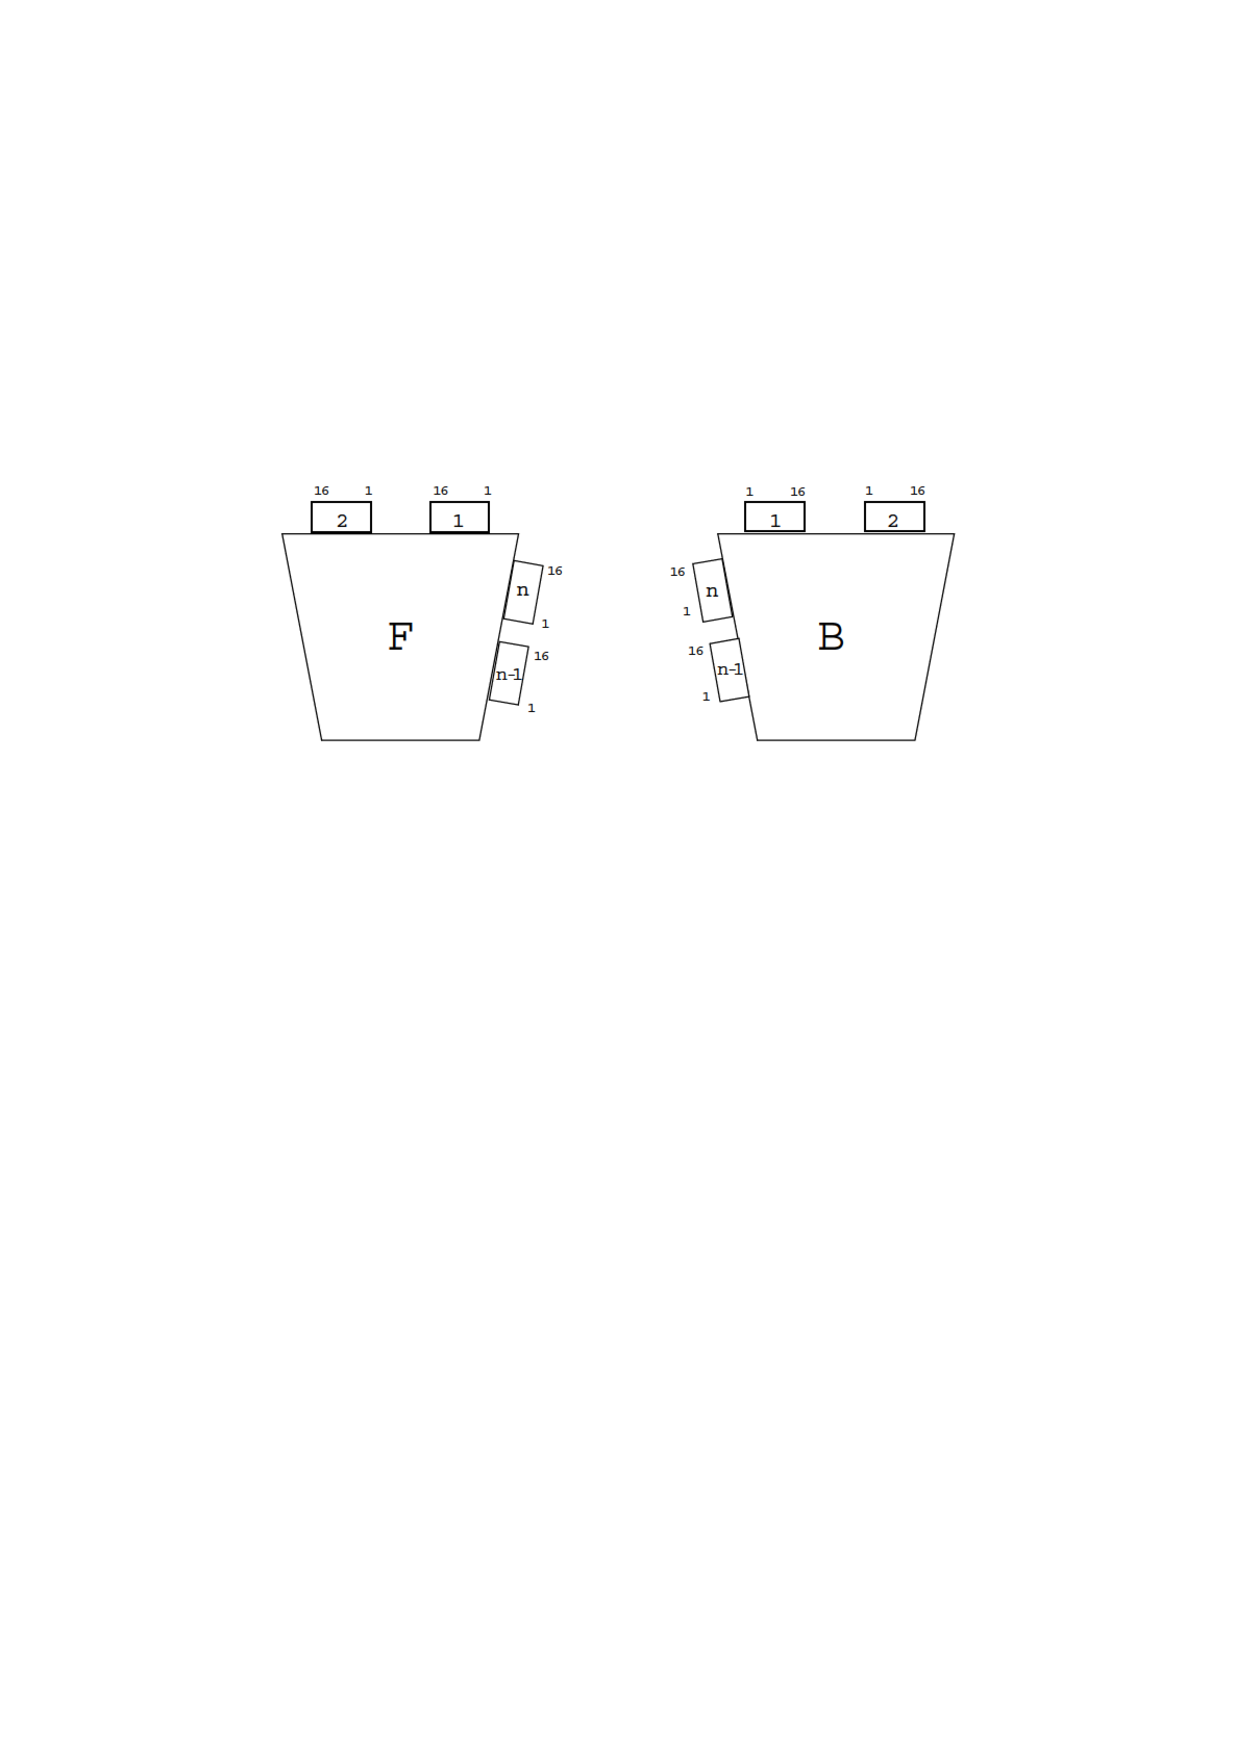
\includegraphics[width=0.8\textwidth,page=1]{img/pdf/TGC.pdf}
        \caption[フロントエンドエレクトロニクス、ASD~および~ボードを搭載したフォワードユニットとバックワードユニット]{フロントエンドエレクトロニクス、ASD~および~ボードを搭載したフォワードユニットとバックワードユニットを初期相互作用点から見た様子~\cite{TR:02}。}
        \label{fig:tgcBF}
\end{figure}

\begin{table}[tb]
	\centering
	\begin{tabular}{c|llll}\hline
		 ユニット & メジャータイプ & B/F & ステーション & マイナータイプ \\ \hline
		 &01..11& B = Backward & 1 = M1~(triplet)~& I = Integral \\
		 && F = Forward  & 2 = M2~(doublet)~& H = Hollowed \\
		 &&              & 3 = M3~(doublet)~& S = Short    \\
		 &&              & 4 = EIFI~(doublet)~& \\ \hline
	\end{tabular}
	\caption[TGC~におけるユニットの型名命名法]{TGC~におけるユニットの型名命名法~\cite{TR:02}。}
	\label{tb:unit1}
\end{table}

\subsubsection{チャンネルナンバリング}
doublet~の場合、ワイヤーとストリップの両方が、フロントエンドエレクトロニクスによって完全に読み出される。triplet~3~層の内、中央のチェンバーでは、ワイヤーのみが読み出される。
コネクタのチャンネル番号と整合性をとるため、以下のような規則にしたがって~ASD~ボードを通してチェンバーから~1~から~n~までのチャンネル番号がつけられている。\figref{fig:tgcT}に~TGC~ユニットにおける構成およびチャンネルの番号の詳細について示す。
\begin{itemize}
\item ワイヤー: \\
チャンネル~1~は、ビームに最も近い~(つまり台形の小さな底面に近い)~。
\item ストリップ: \\
チャンネル~1~は、ワイヤーの~ASD~ボックスの側面に最も近い。したがって、初期相互作用点に座って検出器のホイールを観察している観察者にとって、ストリップの読み出しは、後方検出器の場合は時計回りに、前方検出器の場合は反時計回りに進む。
\end{itemize}

\begin{figure}[H]
		\begin{minipage}{0.49\hsize}
		\centering
        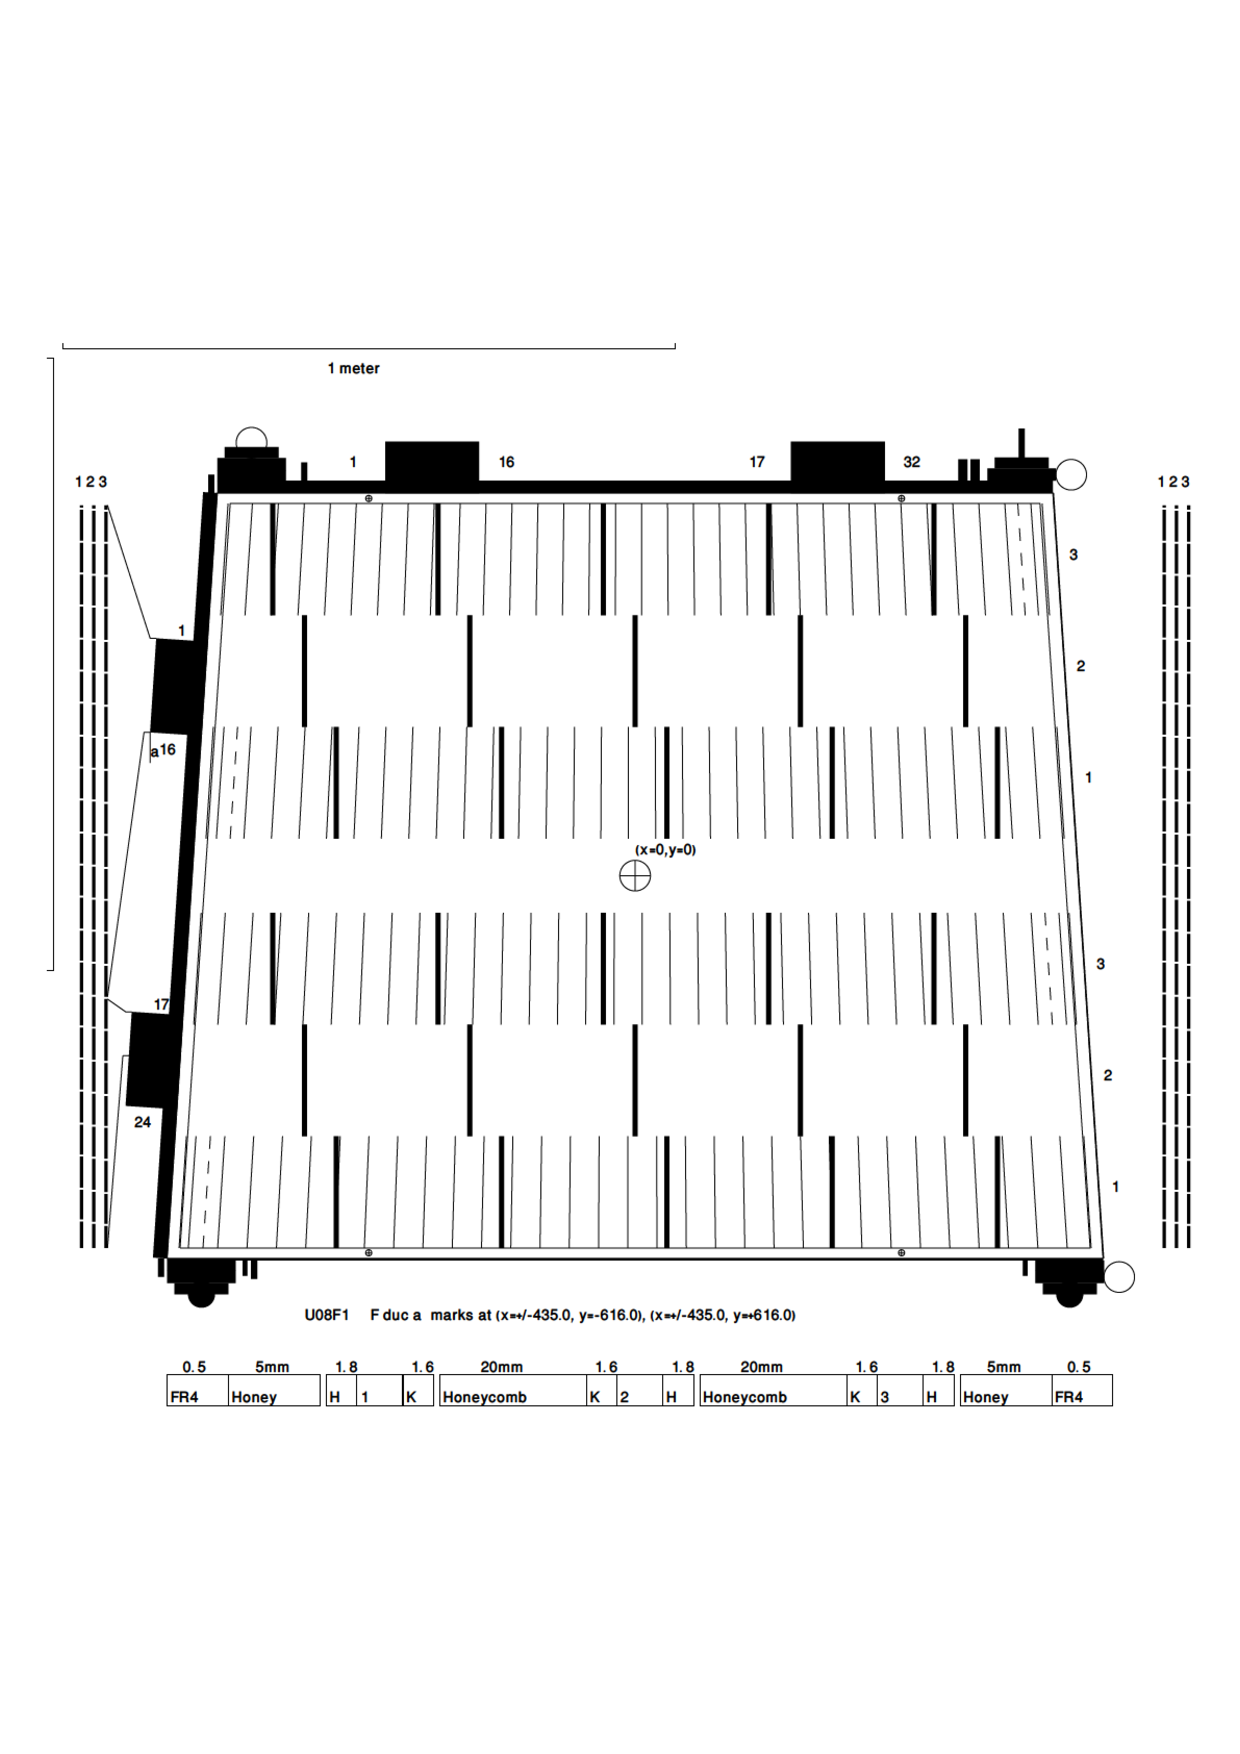
\includegraphics[width=0.9\textwidth]{img/pdf/u08f1i.pdf}
        \subcaption{}
        \end{minipage}
        \begin{minipage}{0.49\hsize}
        \centering
        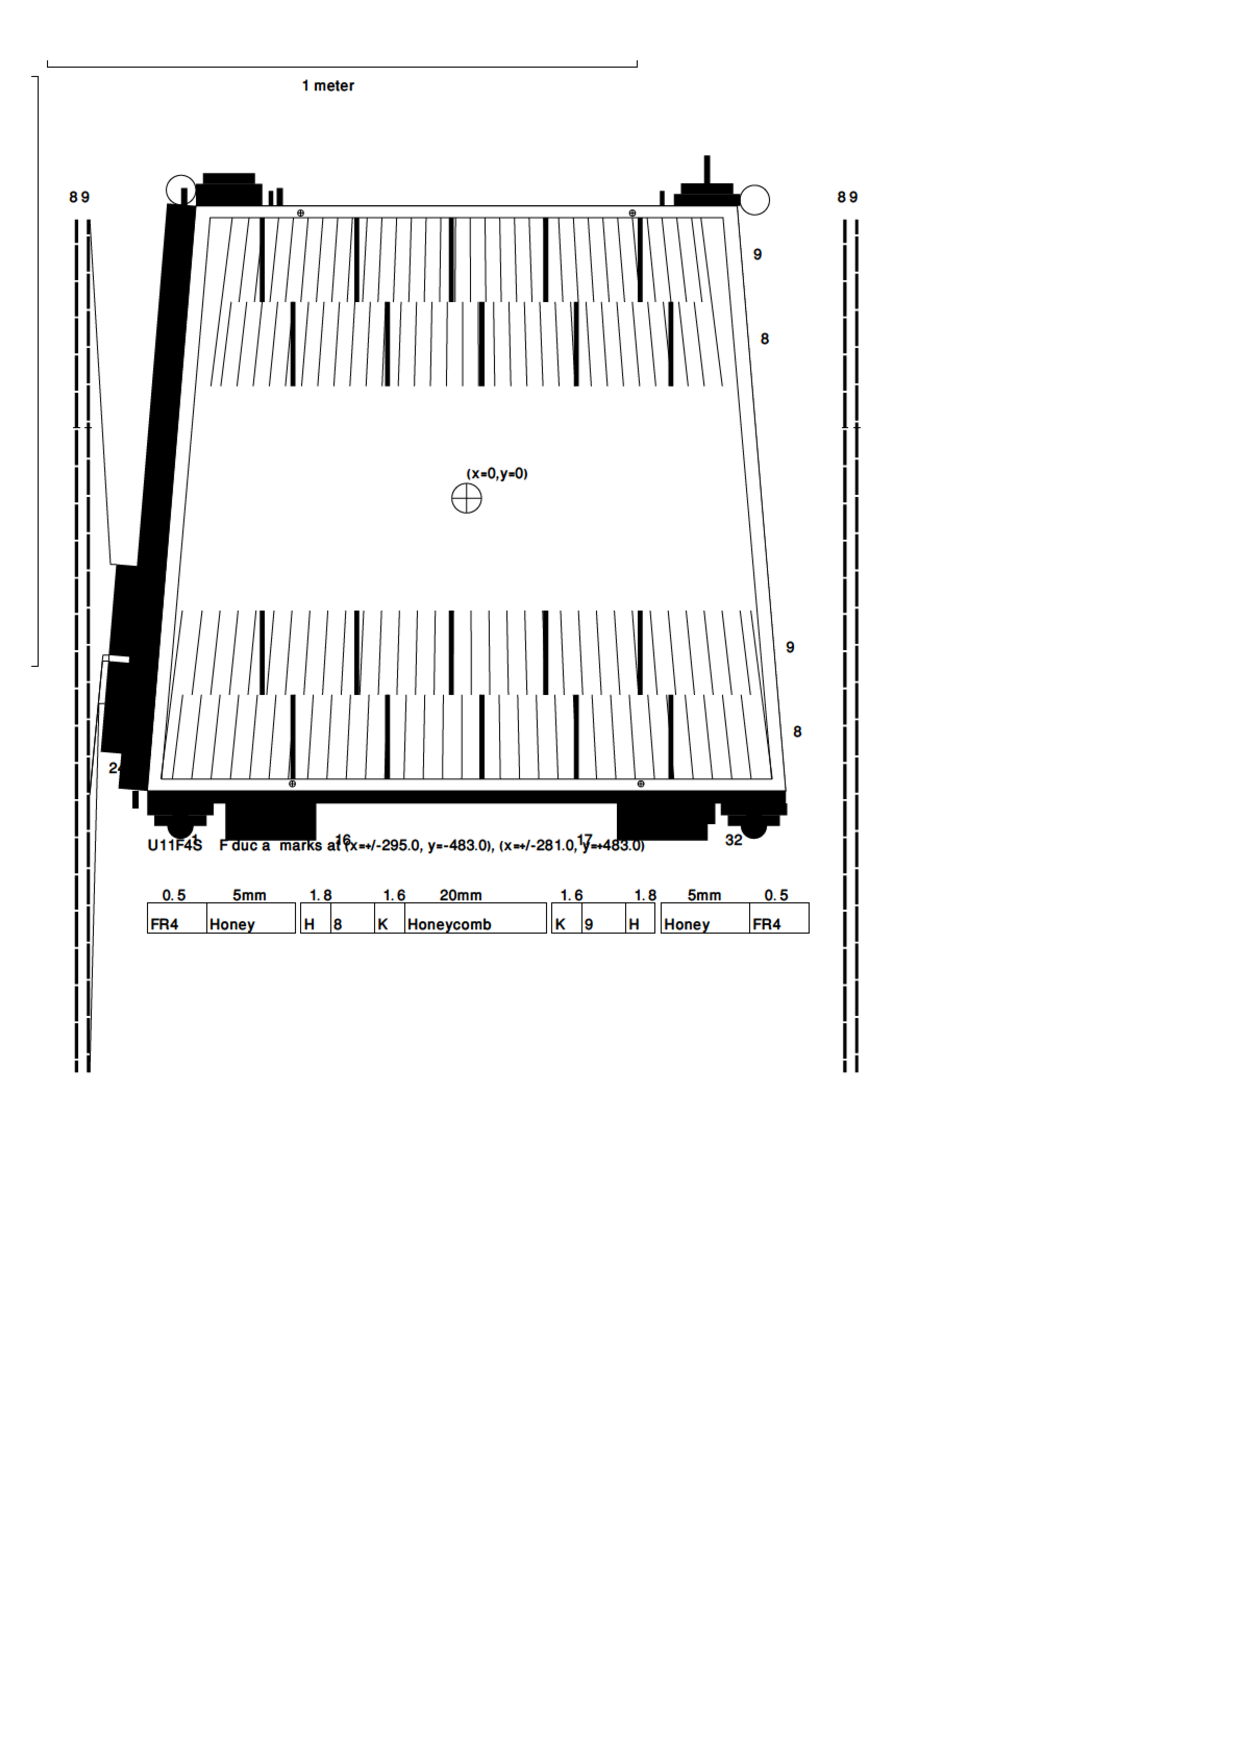
\includegraphics[width=0.9\textwidth]{img/pdf/u11f4s.pdf}
        \subcaption{}
        \end{minipage}
        \caption[TGC~検出器の構成の一例]{TGC~検出器の構成の一例~\cite{URL:04}。図の縦方向にストリップセンサー、横方向にワイヤーセンサーが設置されている。またワイヤーおよびストリップ方向にそれぞれ~2~つの~ASD~が設置されている。チャンネルナンバリングについても記載している。(a)~T08~チェンバーにおける~F1I~ユニット。(b)~T11~チェンバーにおける~F4S~ユニット。}
        \label{fig:tgcT}
\end{figure}

\subsubsection{TGC~のジオメトリの概要}
TGC~システムは、互いに鏡像となる~A~と~C~の~2~つの側面で構成されている。A~は$+z$軸側、C~は$-z$軸側である。トンネルの傾斜~($1.23\%$)~のため、C~は~A~より約~30~cm~上に位置している。これは標準的な~ATLAS~の座標系である。
TGC~セグメンテーションは以下の通りである。
\begin{itemize}
    \item $\eta$ には、2 つの完全に独立した領域が存在する。フォワード ($1.6<|\eta|<2.0$) と エンドキャップ ($1.0<|\eta|<1.6$)。
    \item フォワード領域の $\phi$ 分割は 24~(検出器角度分割 = 15$^{\circ}$)。
    \item エンドキャップ領域の最小の $\phi$ 分割は 48~(検出器角度分割 = 7.5$^{\circ}$)。
    \item エンドキャップ領域のユニットは、半径方向に 4 台~(M1)~および 5 台~(M2、M3)~の「モジュール」~(ラダー)~に組み立てられる。
    \item エンドキャップ領域では、2つのモジュールはさらに2×4または2×5の「セット」にグループ化される。このグループのうち、一方は~Backward ユニット、もう一方は~Forward ユニットで構成される。フォワード領域では、各ユニットはモジュールであると同時にセットでもある。
    \item 1つのフォワード検出器と1つのエンドキャップ・セットのユニットのアセンブリは、それ自体がセットと呼ばれ、基本的な物理的アセンブリとなる。
\end{itemize}
\tbref{tb:tgcNaming}、\tbref{tb:4tgc}に TGC のジオメトリにおける詳細な位置の命名法をまとめる。

\begin{table}[tb]
	\centering
	\begin{tabular}{llll}\hline
	A/C & ステーション & E$i$/F & $\phi$ \\ \hline
	Side & 1 = M1  & E1 = エンドキャップの最も外側 & 0..23~(フォワード)~\\
	& 2 = M2 & E4 or E5 = エンドキャップの最も内側 & 0..47~(エンドキャップ)~\\
	& 3 = M3 & F = フォワード & \\
	& 4 = EIFI && \\ \hline
	\end{tabular}
	\caption{TGC の命名法}
	\label{tb:tgcNaming}
\end{table}

\begin{table}[tb]
	\centering
	\begin{tabular}{c|cccccc}\hline
	& \multicolumn{6}{|c}{$|\eta|$ ---------------------->} \\
	ステーション & E1 & E2 & E3 & E4 & E5 & F \\ \hline
	1 = M1 & T08 & T07 & T06 & T03 & & T01 \\
	2 = M2 & T09 & T08 & T07 & T06 & T04 & T02 \\
	3 = M3 & T09 & T08 & T07 & T06 & T05 & T02 \\
	4 = EIFI & T11 &&&&& T11 \\ \hline
	\end{tabular}
	\caption{各ステーションにおけるメジャータイプの割り当て}
	\label{tb:4tgc}
\end{table}

\section{TGC~での運動量概算}
エンドキャップのミューオントリガーシステムは、BW~における~7~層の~TGC~検出器のコインシデンスを利用している。さらに~7~層の検出点の位置情報を利用した運動量の概算により、運動量のラベル付けを行ったコインシデンス情報を出力できるトリガー系となっている。\figref{fig:tgcpt}に$p_{\rm{T}}$の大きさによって変化する飛跡の一例を示した。

また、\figref{fig:tgcptt}は~TGC~における運動量概算の概念図である。エンドキャップ領域のミューオントリガーシステムにおける運動量の概算方法としては、全検出層が磁場の外にあり磁場中のトラックの曲率を直接測ることはできないため、代わりに~7~層の~TGC~検出器を用いて再構成した直線飛跡を用いて運動量を概算を行う。TGC~トリガー回路系は複数層のヒットコインシデンスに基づき直線飛跡を再構成し、衝突点を向いたトラックを選ぶことで、高運動量のミューオンを選別するトリガーとして機能する。この手法を~Point-Angle~Measurement~と呼ぶ。

7~層のTGC~検出器、M1、M2、M3~はそれぞれ$\it{z}=\rm{13}~\rm{m},~\it{z}=\rm{14}~\rm{m},~\it{z}=\rm{14.5}~\rm{m}$に位置している。TGC~はワイヤーとストリップの直交した二つの読み出しから荷電粒子の通過位置を決定する。ワイヤーが$\eta$方向を測定し、ストリップが$\phi$方向を測定する。必要十分な位置分解能を達成するためのチャンネル幅は~ワイヤー、ストリップともに$\mathcal{O}(1~\rm{cm})$となっている。トリガーロジックは~M3~におけるヒットを~Pivot~として用いて~Point-Angle~Measurement~を行う。

また、エンドキャップトロイド磁石よりも衝突点に近い側に位置する~EIFI~とのコインシデンスを取ることで、衝突点から飛来したミューオンに対して選択的にトリガーを行なっている。

\begin{figure}[H]
        \centering   
        \includegraphics[width=\textwidth,page=13]{img/pdf/ATLAS.pdf}
        \caption[初段エンドキャップミューオントリガーにおけるミューオンの飛来の様子と~RoI~の詳細]{初段エンドキャップミューオントリガーにおけるミューオンの飛来の様子と~RoI~の詳細~\cite{TR:01}。左図は~TGC~検出器の断面図であり、ミューオンの$p_{\rm{T}}$の大きさによるふるまいの違いを示している。右図は~TGC~のトリガーセクターと~RoI~を表しており、緑の線で囲まれた部分が~1~トリガーセクターを示す。赤で囲まれた部分が~1~RoI~を表す。}
        \label{fig:tgcpt}
\end{figure}

\begin{figure}[H]
        \centering   
        \includegraphics[width=0.9\textwidth,page=1]{img/pdf/pttgc.pdf}
        \caption[TGC~BW~におけるミューオンの運動量概算の概念図]{TGC~BW~におけるミューオンの運動量概算の概念図~\cite{MT:03}。ミューオンが残すヒット点と直線飛跡との$R,~\phi$方向との差からミューオンの横運動量を概算する。}
        \label{fig:tgcptt}
\end{figure}

TGC~検出器は~Triplet~内、Doublet~内のローカルなコインシデンスをもちいてデータリダクションを行い、最終的に~3~ステーションコインシデンスによりトリガー判定を行う。手順は以下の通りである。
\begin{itemize}
\item ミューオンが通過し、7~層のワイヤーと~6~層のストリップにそれぞれヒットを残す。
\item ステーション内の~2~層または~3~層のコインシデンスをもちいてノイズのヒットをのぞき、かつコインシデンス結果より各ステーションにおける通過位置を$R$,$\phi$で別々に求める。
\item M2、M3~の間でのコインシデンスをとって~Doublet~4~層でのトラックセグメントを求める。このとき$dR_{23}=R_2-R_3$、$d\phi_{23}=\phi_2-\phi_3$が運動量の指標として用いられ、小さいものだけをトラック候補として残す。
\item M2、M3~のコインシデンス結果と~M1~の間で、さらにコインシデンスをとる。M2、M3~の間のコインシデンスで行なったように、$dR_{13}=R_1-R_3$と$d\phi_{13}=\phi_1-\phi_3$の情報を用いてトラック候補の選別を行う。ここまではワイヤー($R$)~とストリップ($\phi$)は別々に計算される。
\item 最後に、$R$と$\phi$の情報のコインシデンス情報を合わせて、RoI~を形成し、さらに$dR$および$d\phi$の情報を合わせて運動量判定を行う。この運動量判定情報および~RoI~の情報が~MUCTPI~に送られる。
\end{itemize}

\section{TGC~エレクトロニクス}
TGC~システムの電気回路系におけるデジタル電気回路の設置箇所は大きく以下の~3~つに分かれる。
\begin{itemize}
    \item PS Board: \\
    Patch~Panel~ASIC~(PP)~と~Slave~Board~ASIC~(SLB)~が設置されている。
    \item ミニラック:\\
    読み出し用のモジュールである~Star~Switch~(SSW)~と、M1、M2、M3~のコインシデンスのための~High-PT~board~(HPT)~が搭載されている。
    \item USA15: \\
    USA15~に読み出しのための~Readout~Driver~(ROD)~モジュールが設置されており、SSW~からのデータを受信する。Sector~Logic~(SL)~は~HPT~の$R$コインシデンスと$\phi$コインシデンスの結果を合わせ~RoI~と$p_{\rm{T}}$判定を行うモジュールである。またクレートを遠隔でコントロールするために、CCI~と呼ばれるモジュールが設置されている。LHC~クロックを受信してフロントエンド電気回路に配布する~TTC~(Trigger~Timing~Control)~システムも~USA15~に配置している。TTC~システムは~LHC~クロックに加えて~Event~Counter~Reset~(ECR)~や~Bunch~Counter~Reset~(BCR)~信号および~L1A~の配布も行う。
\end{itemize}
\figref{fig:tgcelec}~TGC~システムの電気回路系におけるトリガー信号とリードアウトチェーンの流れを示す。
また、以上の電気回路系は大きく次の~4~つのパスに分かれている。
\begin{itemize}
    \item トリガー系
    \item リードアウト系
    \item コントロール系
    \item トリガータイミングコントロール系
\end{itemize}
次節以降にこれらの詳細について記す。

\begin{figure}[H]
        \centering   
        \includegraphics[width=0.9\textwidth,page=14]{img/pdf/ATLAS.pdf}
        \caption[TGC システム電気回路系におけるトリガーとリードアウトチェーンの流れ]{TGC~システム電気回路系におけるトリガーとリードアウトチェーンの流れ~\cite{TR:01}。TGC~のフロントエンドにあるエレクトロニクスによって~TGC~BW~の~ワイヤー~($R$)、ストリップ~($\phi$)~のそれぞれでコインシデンスがとられたのち、バックエンドにある~セクターロジックボードによって、ワイヤー、ストリップ間コインシデンスおよび~TGC~EIFI~とタイルカロリメータとのコインシデンスがとられる。}
        \label{fig:tgcelec}
\end{figure}

\subsection{リードアウト系}
\subsubsection{Amplifier~Shaper~Discriminator~(ASD)~}
\label{subsubsec:ASD}
ASD~は~TGC~検出器のセンサー~(ワイヤー、ストリップ)~からの生の電流信号を電圧信号に変換し、増幅されたのちにコンパレータにかけられ~LVDS~レベルの信号~(作動信号)~を出力する役割を持つ。出力信号は~Patch-Panel~に届けられる。ASD~ボードは各チェンバーに対して共通した作りになっており、4~チャンネルの信号を処理できるチップが~4~枚搭載されている。したがって~ASD~ボード一つ当たり~16~チャンネルの信号処理が可能となっている。ASD~はチャージアンプである前段増幅器~(電圧変換効率はピークで~0.8~V/pC)、利得~7~倍の作動電圧増幅回路、コンフィギュレーション可能な閾値電圧とのコンパレータからなる。作動電圧増幅回路の出力が閾値電圧を超えている時間だけのパルス長で~LVDS~のデジタルパルスが出力される。\figref{fig:ASD}に~ASD~チップの詳細を示す。また\figref{fig:signal}にASD~における信号波形シミュレーションの結果を示す。

\begin{figure}[H]
		\begin{minipage}{0.49\hsize}
		\centering
        \includegraphics[width=0.8\textwidth,page=3]{img/pdf/ASD.pdf}
        \subcaption{}
        \end{minipage}
        \begin{minipage}{0.49\hsize}
        \centering
        \includegraphics[width=0.8\textwidth,page=4]{img/pdf/ASD.pdf}
        \subcaption{}
        \end{minipage}
        \caption[ASD~チップの詳細]{(a)~4~チャンネル~ASD~チップの写真~\cite{URL:06}。サイズは、$3.1~\rm{mm}~\times~3.1~\rm{mm}$。(b)~ASD~IC~チップにおけるピンアサインメント~\cite{URL:06}。}\label{fig:ASD}
\end{figure}

\begin{figure}[H]
        \centering   
        \includegraphics[width=0.9\textwidth,page=2]{img/pdf/ASD.pdf}
        \caption[ASD~の信号波形シミュレーション]{ASD~の信号波形シミュレーション~\cite{URL:06}。左図は$\rm{-0.5\sim-0.1}~\rm{pC}$の差動信号入力、右図は$\rm{0.1\sim0.5}~\rm{pC}$の差動信号入力である。上図はプリアンプ出力、中図は~2~つのメインアンプ差動出力信号、下図は~2~つのコンパレータ差動出力信号~(LVDS)~である。}
        \label{fig:signal}
\end{figure}

\subsubsection{PS-Board}
PS-Board~には~Patch-Panel~ASIC~と~Slave~Board~ASIC~が搭載されている。全部で~17~種類のボードが存在する。ASD~から信号を受信し、バンチ交差識別および信号間のコインシデンス処理を行い、HPT~にトリガー情報、SSW~にリードアウト情報を送信する。また~ASD~ボードに対して~DC~電源、閾値電圧の供給を行う。

\subsubsection{Patch-Panel~ASIC}
Patch-Panel~ASIC~(PP)~は~ASD~が出力した~LVDS~信号を受けて、入力信号のタイミングを揃えたのち~40~MHz~のクロックでサンプリングを行う。\figref{fig:PPphoto}に~PP~の写真を示す。

\begin{figure}[H]
        \centering   
        \includegraphics[width=0.5\textwidth,page=2]{img/pdf/PP.pdf}
        \caption[PP ASIC の写真]{PP ASIC の写真~\cite{URL:05}。サイズは$5~\rm{mm}~\times~5~\rm{mm}$。}
        \label{fig:PPphoto}
\end{figure}

LVDS~入力信号の時間分布はミューオンの衝突点から検出器までの飛行時間~(Time-of-Flight)、ASD~から~PP~までの~LVDS~ケーブルの長さ等の要因によりチャンネル毎に異なる。以上のような遅延要因は一つのチャンネルに対する共通したオフセットである。このオフセットはチャンネル毎に信号遅延を調整すれば対応可能なものであるが、ASD~は~16~チャンネル毎の処理のため非合理的である。また、同一チャンネルにおいてもミューオンの入射位置により伝搬時間が異なるために生じるタイミングの差異や、ミューオンがガスを電離し電流信号となるまでにかかるドリフト時間により内在的なタイミングのふらつきが生じる。ある程度のタイミングの揺らぎは許容し、時間分解能を評価した上で信号線の遅延やゲート幅の調整を行うことが重要である。

遅延を行うための回路には、PP~に含まれる~Fine~Delay~(0.83~ns~ステップ)、ゲート回路、また下流の~Slave~Board~の入力にある~Coarse~Delay~(25~ns~ステップ)~がある。
PP~は~2~つの独立なパート~Port-A、Port-B~に分けられており、それぞれ~PP~16~チャンネルの入力に対応している。これは~ASD~1~枚の出力と対応している。\figref{fig:delay}に入力信号に対する遅延のかけ方のイメージ図を示した。

Fine~Delay~のあとに、Mask~とゲート回路が搭載されている。
Mask~は信号のタイミングを揃えるために出力を制限する場合や、信号のノイズが大きい等の不良が発生する場合、後段への信号送信をチャンネル毎に制御することができる機能である。\figref{fig:PP}に~PP~ASIC~における信号処理の流れを示した。
\begin{figure}[H]
        \centering   
        \includegraphics[width=0.65\textwidth,page=1]{img/slide/slide.pdf}
        \caption[信号タイミング調整の概念図]{信号タイミング調整の概念図~\cite{URL:09}。ケーブル~1,~2,~3~における入力タイミングの確率分布を示している。タイミング調整はケーブル単位で可能であり、一番遅く到達する時間に合わせる。}
        \label{fig:delay}
\end{figure}

\begin{figure}[H]
        \centering   
        \includegraphics[width=\textwidth,page=1]{img/pdf/PP.pdf}
        \caption[PP ASIC での信号処理の流れ]
        {PP ASIC での信号処理の流れ~\cite{URL:05}。入力信号に対して遅延がかけられ、Mask~およびバンチ交差識別が行われる。}
        \label{fig:PP}
\end{figure}

\subsubsection{バンチ交差識別}\label{subsubsec:bcid}
PP~では~TGC~のヒット信号の立ち上がりを検出し、バンチ判定を行う。一つのインプットに対して、2~バンチのヒット情報を出すわけではない。TGC~ゲートはクロックの立ち上がりのタイミングと同期する。したがって同期したゲート幅内に~TGC~の生信号の立ち上がりが来るように幅を定義している。\figref{fig:clock}に信号の時間分布に対するクロック位相の調整方法についてを示す。

TGC~出力信号は内在的な時間の揺らぎの影響で陽子衝突間隔~25~ns~より大きい。特にストリップではセンサーの長さとドリフト時間の影響が大きい~(約~30~ns~(ワイヤー)、約~40~ns~(ストリップ)~)~。そのため信号の時間分布に対して、十分なゲート幅ならびにノイズ等の影響を鑑みて最小限のゲート幅を確保することが非常に重要である。\figref{fig:gate0}に例として信号の時間分布に対するゲート幅の調整方法についてを示す。図中の三角形は、1~事象の波形ではなく、バンチ交差を起点に~PP~で検出される信号の立ち上がり時間の確率分布関数を示していて、この分布の幅が内在的な時間分解能を表している。TGC~におけるゲート幅は可変~($\rm{26\sim48~ns}$)~で~PP~において決められた幅が設定されている。\figref{fig:bcidgate}は可変なゲート幅を最小および最大に設定した場合のゲートの状態を示したものである。Run~2~におけるゲート幅の設定は\tbref{tb:BCIDGate}のようになっている。

以上の要領で設定された電子回路によりバンチ交差識別を行う。バンチ判定は\figref{fig:bcid0}のような概念図として表すことができる。25~ns~おきの~LHC~クロックに対して、前バンチ、基準バンチおよび次バンチのゲートが設定されている状態である。そして\tbref{tb:BCIDGate}に示したようにゲート幅は、25~ns~よりも大きな幅がとられている。これはゲートに重なりを持たせることで不定性の削減を行うためである。したがって~TGC~におけるバンチ判定は、前バンチ、前かつ基準バンチ、基準バンチ、基準かつ次バンチ、次バンチの~5~段階で行われる。光速のミューオンは信号の時間的揺らぎを考慮した上で基準バンチで判定されるように調整されている。

\begin{figure}[H]
        \centering   
        \includegraphics[width=0.8\textwidth,page=2]{img/slide/slide.pdf}
        \caption[クロック位相の調整]{クロック位相の調整~\cite{URL:09}。40~MHz~の~LHC~クロックの立ち上がりに対して、入力タイミングの確率分布の始まりを合わせるように位相を調整している。}
        \label{fig:clock}
\end{figure}
\begin{figure}[H]
        \centering   
        \includegraphics[width=0.9\textwidth,page=3]{img/slide/slide.pdf}
        \caption[BCID~ゲート幅の調整]{BCID ゲート幅の調整~\cite{URL:09}。入力タイミングの確率分布がすべて収まるように、BCID~ゲートの幅が調整されている。}
        \label{fig:gate0}
\end{figure}
\begin{figure}[H]
        \centering   
        \includegraphics[width=0.7\textwidth,page=4]{img/slide/slide.pdf}
        \caption[バンチ判定の概念図]{バンチ判定の概念図。LHC~クロックに対してゲートが設定されており、入力信号のタイミングにより、前バンチ、前かつ基準バンチ、基準バンチ、基準かつ次バンチ、次バンチの~5~段階で判定が行われる。}
        \label{fig:bcid0}
\end{figure}

\begin{table}[tbp]
	\centering
	\begin{tabular}{c|l}\hline
	& \multicolumn{1}{c}{ゲート} \\ \hline
	BW ワイヤー & 29.32 ns~(26 ns + 4 × 0.83 ns)~\\
	BW ストリップ & 40.94 ns~(26 ns + 18 × 0.83 ns)~\\
	SW ワイヤー & 33.47 ns~(26 ns + 9 × 0.83 ns)~\\
	SW ストリップ & 45.09 ns~(26 ns + 23 × 0.83 ns)~\\ \hline
	\end{tabular}
	\caption{Run~2~におけるゲートの設定値}
	\label{tb:BCIDGate}
\end{table}

\begin{figure}[H]
		\begin{minipage}{0.49\hsize}
		\centering
        \includegraphics[width=0.9\textwidth,page=3]{img/pdf/PP.pdf}
        \subcaption{}
        \end{minipage}
        \begin{minipage}{0.49\hsize}
        \centering
        \includegraphics[width=0.9\textwidth,page=4]{img/pdf/PP.pdf}
        \subcaption{}
        \end{minipage}
        \caption[ゲート幅の調整]{ゲート幅の調整~\cite{URL:05}。(a)~ステップが~0~(最小)~の場合。(b)~ステップが~26~(最大)~の場合。}
        \label{fig:bcidgate}
\end{figure}

\subsubsection{Slave~Board~ASIC}
Slave~Board~ASIC~(SLB)~は~TGC~出力信号のコインシデンス処理ならびに読み出し処理を行う役割を持ち、トリガー系とリードアウト系に区分される。以下では、リードアウト系に関する事項について説明する。

SLB~は~160~bits~の入力ポートを持ち、最大~160~チャンネルのヒットパターンが入力される。リードアウト系における~SLB~の役割は、受信した~160~bits~の情報を~L1A~を受け取るまで一時的にバッファにデータを保持しておくことである。
L1A~の信号を受信した後には、対応するデータに加えて前後$\pm1$バンチの情報も読み出し、それぞれ~Previous~(前バンチ)、Current~(基準バンチ)、Next~(次バンチ)~とタグ付けして~Star~Switch~に送信する。

\subsubsection{Star~Switch}
Star~Switch~(SSW)~は複数の~PSB~からの信号を~RDO~へと送信する役割を持つ。この際、転送するデータ量を減らすためにヒットがない情報は省く~(zero-suppress)~。SLB~からのデータはレシーバーに入力されデータの圧縮を行う。その後、トランスミッターに送信されフォーマットされる。フォーマットされたデータはシリアライズされ、RDO~に送られる。

\subsubsection{Read-Out~Driver}
Read-Out~Driver~(ROD)~は複数の~SSW~からシリアライズされた圧縮データを受信し、パラレルデータに戻しメモリーに一時格納する。このデータを、トリガー情報をもとに同一事象毎にまとめる。まとめられたデータは~S-LINK~という光信号で~ROS~に送信される。イベント同定のためには~TTC~からのトリガー情報が必要となるため、ROD~には受信のための~TTC~Receiver~Chip~(TTCrx)~が搭載されている。

\subsection{トリガー系}
TGC~のトリガーはバンチ交差識別された事象のセットを利用し、複数段のコインシデンス論理により、データサイズを減らしながら、コインシデンスロジックに用いる総数を増加させていくことで、最終的に~3~ステーションコインシデンスで~RoI~の決定および運動量の概算を行う。
\subsubsection{Slave~Board~ASIC}
バンチ交差識別が行われ~LHC~クロックでサンプリングされたヒットは、L1~Buffer~に詰め込まれると同時に、SLB~のトリガーロジックに入力される。SLB~のトリガーロジックでは以下の演算を行っている。
\begin{itemize}
\item 2~層内、3~層内のコインシデンスおよびスタッガリングを用いた分解能の向上
\item M2,~M3~の間の~4~層でのコインシデンス
\end{itemize}
1~チップで各チェンバーの~32~チャンネルを処理する。チャンネルの種類の応じて~5~種類のコインシデンスマトリックス~(ワイヤーdoublet、ストリップdoublet,ワイヤーtriplet、ストリップtriplet,~EIFI)~を切り替えて利用している。$\eta$方向に見た場合、TGC~の~doublet~内及び~triplet~内でスタッガリング構造~(層ごとに~TGC~の位置が少しずれて配置されている)~を持つため、コインシデンスによりデータ量を減らすのみでなく、位置分解能の向上にも起因する。
triplet~のワイヤーSLB~トリガー回路では、3~層内でのコインシデンス処理を行う。3~層中~2~層のヒットを要求し、3~層の生信号を利用して~M1~に代表するヒットポイントを計算する。このロジックは~1~clock~サイクルで十分に終わることができるような設計となっている。ヒット情報の入力後、次のクロックの立ち上がりに演算結果が出力され~HPT~に送信される。複数のコインシデンス結果が見つかった場合は、代表するヒットを選び出すロジックの実装により~1~clock~で送信できるような設計になっている。同様にストリップSLB~のトリガー回路は、M1~の~2~層中~1~層を要求するロジックで実装されている。
doublet~の~SLB~は、M2~と~M3~の~4~層を担当している。まず、M2~と~M3~の間で~2~層中~1~層のコインシデンス処理を行い、M2,~M3~で~4~層中~3~層のコインシデンスがとられる。

\subsubsection{High-PT~Board}
High-PT~Board~(HPT)~は~SLB~の出力を用いて、doublet~(M2-M3)~,triplet~(M1)~の間のコインシデンス処理を行う。SLB~のトリガー出力情報には以下が含まれている。
\begin{itemize}
\item M1~のヒット点の情報~($R_1,~\phi_1$)~
\item M3~のヒット点の情報~($R_3,~\phi_3$)~と、M2-M3~の差分~($dR_{32},~d\phi_{32}$)~
\end{itemize}
$R$方向のワイヤーコインシデンスと、$\phi$方向のストリップコインシデンスが別々に実行される。
SLB~と同様に、コインシデンスマトリックスを用いて計算は行われ、計算は~1~clock~サイクルで完了する。M1~と~M3~の間でコインシデンス処理を行い、
$|dR_{13}| \leq 15,~|d\phi_{13}| \leq =7$の条件をクリアした候補~(トラックレット)~が~Sector~Logic~(SL)~に送信される。
\subsubsection{Sector~Logic}
TGC~トリガーの最終段は~Sector~Logic~Board~(SL)~で、$R$~(ワイヤー)~と$\phi$~(ストリップ)~の独立な~HPT~出力を統合して、$p_{\rm{T}}$情報を概算し、RoI~と$p_{\rm{T}}$情報をパックして、MUCTPI~に送信する。HPT~の出力には、~($R_{3},~dR_{13}$)~,~($\phi_{3},~d\phi_{13}$)~が含まれるため、$R_3,~\phi_3$の情報をもとに、RoI~が決定され、$dR_{13},~d\phi_{13}$の情報をもとに$p_{\rm{T}}$が概算される。$p_{\rm{T}}$閾値に変換する過程は、高速処理のためあらかじめ変換の計算を対応表にした~Look-Up~Table~によって行われる。1~つのトリガーセクターから~1~バンチ~2~RoI~まで出力することができる。

\subsection{コントロール系}
デジタル電気回路の制御は、電子回路に組み込まれたレジスタ~(メモリ)~の読み書きによって行われている。レジスタに対する命令による電気回路の動作決定や、値を読み出すための命令による電気回路の状態のモニターなどの役割を持つ。

\subsection{トリガータイミングコントロール系}
ATLAS~実験では~40~MHz~という高頻度衝突かつ広範囲に設置された検出器による影響で、全体での事象の同期は容易ではない。同期のために大きな役割を担っているのが、TTC~システムである。各検出器では事象の情報を読み出すために~L1A~を受信する必要がある。なおかつ事象を正しく識別するためには~LHC~の衝突との同期を行わなければならない。そのため~BC~clock~(Bunch~Crossing~signal)~を各検出器に配布している。事象の認識のために読み出しが行われた情報に対しては~EVID~および~BCID~が付与される。

実験全体を通して以上の~ID~の一貫性を保つためには、システム全体を同期する基準となる信号が必要である。それらの信号を~BCR~(Bunch~Counter~Reset)~と~ECR~(Event~Counter~Reset)~と呼ぶ。TTC~信号を送信するのは、各検出器に設置されている~TTCvi~(TTC~VME~interface)~である。TTCvi~から送信された信号は光ファイバーを通して~TTCrx~(TTC~Receiver~Chip)~に送られる。TTCrx~ではタイミング調整のために~TTC~信号に対してクロック位相を~100~ps~の単位で調節でき、L1A~や~BCR,~ECR~の信号を~0~15~clock~の範囲で遅延することができる。

\section{TGC~システムにおけるタイミング調整}
本章では、TGC~エレクトロニクスにおける詳細な仕組みについて記した。本節では、エレクトロニクスを正しく動作させる上でのタイミング調整の重要性について説明する。

\subsection{タイミング調整の重要性}
ATLAS~の各エレクトロニクスでは~BCID~と~L1ID~が付加され、TTC~システムから配布された基準信号との同期を取ることで、システム全体での整合性を保つ。
TGC~システムは、TTC~が全測定器に~L1A~を発行するための重要な役割を担っている。TGC~において正しいバンチ交差識別が行われていなければ、検出器全体としての事象の同期に影響を及ぼす。どのバンチ衝突から生じた粒子なのかを正しく識別をするには、各検出器においてタイミングの同期を行わなければならない。したがって~TGC~検出器のタイミング調整はトリガーを行う上で非常に重要な役割を持つ。

\subsection{TGC~システムにおけるタイミングのばらつき}
TGC~システムにおいて正しくバンチ判定を行うには、バンチ衝突に対応して~25~ns~毎に開くゲートに荷電粒子の信号を適切に収めることが必要である。
しかし、ミューオンが衝突点から~TGC~まで届くまでの時間~(Time-of-Flight)~には位置による差があり~(約$\rm{24\sim64~ns}$)、さらに粒子の信号を伝搬するための各ケーブルの長さは、位置によって様々であるため、細かなタイミング調整を行わなければ、ゲート幅~($\rm{26\sim48~ns}$)~に収まらない。\figref{fig:tof}に~TGC~の位置によるミューオンの飛来時間の違いを示した。総読み出しチャンネル~32~万の~TGC~におけるタイミング調整を行うには、詳細かつ精密な見積もりが必要となる。またゲート幅に関して、単純に幅を大きくするだけでは、誤ったコインシデンスの増加などが懸念されるため、最小かつ最適なタイミングでゲートを設定することが必要である。

次章では、モンテカルロシミュレーションおよび~Run~2~の実験データを用いて、TGC~検出器におけるタイミング調整の調査を行う。

\begin{figure}[H]
    \centering   
    \includegraphics[width=0.6\textwidth,page=8]{img/slide/slide.pdf}
    \caption{ミューオンの~TGC~各ステーションにおける飛来時間の一例}
    \label{fig:tof}
\end{figure}

\chapter[TGC検出器のタイミング較正と性能改善]{TGC検出器のタイミング較正と\\性能改善}
\thispagestyle{empty}
\label{chap:5}
LHC-ATLAS実験において、信号のタイミング調整は適切にミューオンを捉えるために非常に重要である。40~MHz~(ビーム衝突間隔~25~ns)~という高頻度の陽子衝突から生成されるミューオン等の荷電粒子を捉えるには、ゲート幅の調整や詳細な遅延パラメータの設定が鍵を握る。
\chapref{chap:4}で述べた通り、TGC~検出器では粒子信号の読み取りを適切に行うために、複数の遅延回路が実装されている。
本章では、モンテカルロシミュレーションおよび~2018~年の~Run~2~の実験データを用いて、TGC~検出器のタイミングに関する調査を行い、TGC~エレクトロニクスの設定検証を行う。
TGC~検出器における詳細なタイミング設定に関する理解を深め、Run~3~に向けた性能改善を提案する。

\section{バンチ判定の比較}
本節では、TGC~検出器での測定において得られたバンチ判定の分布およびトリガー判定について説明する。

先行研究において~TGC~でのバンチ判定精度の検証が行われている~\cite{MT:05}。2011~年、LHC~では~50~ns~間隔~(20~MHz)~の陽子バンチ衝突での運転を行った。通常~LHC~クロックは~1~周期~25~ns~なので、50~ns~間隔でのバンチ衝突の場合はクロック~2~周期ごとにバンチ衝突が起こることになる。したがって、2~周期のうち~1~周期分はバンチ衝突が起こらず、トリガーが発行されないような設定となっている。\subsecref{subsec:l1tri}で説明したように、L1~トリガーはパイプライントリガーである。よって、以上の設定においてトリガー判定を正しく行うには、前バンチおよび次バンチでバンチ衝突が起こらないため、基準バンチのタイミングが正しく調整されている必要がある。
また2015~年の運転において、25~ns間隔におけるバンチ判定精度が再び確認された~\cite{kishimoto}。
結果としては、前バンチと判定されるヒットは無視でき、次バンチと判定されるヒットは0.4$\%$程度に抑えられていることが確認された。

\figref{fig:bcid00}に、Run~2~の実験データおよびシミュレーションにおけるバンチ判定の分布の一例を示した。バンチ判定は、\subsubsecref{subsubsec:bcid}で示したように、前バンチ、前かつ基準バンチ、基準バンチ、基準かつ次バンチで識別される。シミュレーションと実験データの分布を比較すると、実験データの方がタイミングの揺らぎが大きく、特に基準かつ次バンチの割合が高いことが分かる。Run~3~の開始に向けて、トリガー判定を損失なく正確に行うには、より詳細なバンチ判定における議論が必要となる。また\secref{sec:latemu}で述べたように次バンチと判定される粒子も新物理探索において重要なファクターとなり、基準バンチのタイミングが正しく調整されていなければ、次バンチで測定される粒子の速度にもばらつきが生じることが考えられる。よって、本研究ではシミュレーションを用いてタイミングの検証を行い~TGC~検出器の詳細なタイミング較正を行う。

\begin{figure}[tbp]
        \centering   
        \includegraphics[width=0.75\textwidth,page=1]{img/pdf5/BCID0.pdf}
        \caption[Run~2~の実験データとモンテカルロシミュレーションにおけるバンチ判定の分布]{Run~2~の実験データとモンテカルロシミュレーションにおけるバンチ判定の分布。FI~T10~チェンバー、ワイヤーチャンネル。}
        \label{fig:bcid00}
\end{figure}

\section{解析のデータサンプル}
本研究に用いた解析のデータサンプルについて説明する。

\subsection{Run~2~の実験データ}
本研究では~Run~2~の実験データとして~2018~年に行われた~Run-2~period~B~の実験データを使用した。
統計量としては、約~400~万事象である。
2018~年には~period~A~から~R~までの運転が行われている。

\subsection{モンテカルロシミュレーション}
シミュレーションに関しては統計量の確保のため、シングルミューオンサンプルを使用した。$3~\rm{GeV}<p_{\rm{T}}<80~GeV$の範囲の横運動量を持つミューオンのサンプルとなっている。統計量としては約~50~万事象である。

ATLAS~実験におけるイベントシミュレーションは、Athena~\cite{URL:21}~と呼ばれるソフトウェアチェーンを用いて行われる。Athena~では複数の段階に分けてデータ処理が行われ、最終的に実験データと同様の解析が行えるように処理されていく。以下では、それぞれの段階におけるシミュレーションの詳細について述べる。

\subsubsection{イベント生成~(Generation)~}
物理事象そのもののシミュレーションを行う。様々なイベントジェネレータが利用されている。

\subsubsection{検出器シミュレーション~(Simulation)~}
生成イベントの粒子の検出器中での振る舞い~(物質との反応や粒子の崩壊など)~を~Geant4~\cite{URL:22}や簡易シミュレーター$\rm{Atlfast-II}$~\cite{TR:08}を用いてシミュレートする。この段階では物質を通過した時刻、場所とそこで落とされたエネルギー損失がデータとして保持される。この状態のデータフォーマットは~Hit~と呼ばれる。

\subsubsection{デジタイゼーション~(Digitization)~}
Hit~データを元に、検出器の信号のシミュレーションを行う。通過時刻、場所とエネルギー損失から信号の発生時間や大きさなどを計算する。その結果はDigitと呼ばれている。Digit~は同等の情報を含むデータフォーマット~Raw~Data~Object~(RDO)~に変換される。Byte~Stream~と呼ばれる実際に取得されたデータもRDOに変換される。

\subsubsection{再構成~(Reconstruction)~}
RDO~を元にトラックやクラスターを再構成し粒子識別を行う。
その結果を~Event~Summary~Data~(ESD)~として保存する。実際には解析のための物理情報を集約した~Analysis~Object~Data~(AOD)~も同時に生成している。

\subsubsection{解析~(Analysis)~}
ESD~や~AOD~を元に、ROOT~\cite{URL:23}等の解析フレームワークで扱いやすい形式にし、ヒストグラム生成等を行う。

\section{TGC~デジタイゼーション}
モンテカルロシミュレーションの~TGC~デジタイゼーションでは、実験におけるバンチ交差識別を再現するために~TGC~検出器内での反応の様々なシミュレーション処理が行われている。ここでは、本研究以前のシミュレーションにおける信号伝搬や遅延等の計算について述べる。シミュレーションにおける信号伝搬の計算について以下にまとめた。

\begin{itemize}
\item 信号伝搬に伴う時間
\begin{itemize}
\item $t_{\rm{ToF}}$:衝突点から各 TGC に到達するまでの時間~(Time of Flight:~ToF)。
\item $t_{\rm{jit}}$:センサーに信号が検出されるまでの時間。
\item $t_{\rm{prop}}$:ワイヤーおよびストリップ において信号が伝播する時間。
\end{itemize}
\end{itemize}
\begin{itemize}
\item 信号遅延
\begin{itemize}
\item $t_{\rm{ToFCor}}$:ToF~による遅延を吸収するための時間。
\item $t_{\rm{offset}}$:信号遅延時間の補正。
\end{itemize}
\end{itemize}

シミュレーションにおいては粒子の生成から信号検出までの伝搬時間を計算している。また信号遅延では、検出までの時間差を吸収するための計算が行われている。すなわち以下の\equref{eq:tdigit}で表される時間とゲートを比較することでバンチ交差識別を行う。

\begin{align}
    \it{t_{\rm{Digit}}=t_{\rm{ToF}}+t_{\rm{jit}}+t_{\rm{prop}}-t_{\rm{ToFCor}}-t_{\rm{offset}}}\label{eq:tdigit}
\end{align}

\section{TGC~検出器のタイミング較正}
Run~2~の実験データ、モンテカルロシミュレーションにおけるタイミングの評価を行う。Run~2~の実験データをより詳細に再現し、シミュレーションのタイミング較正を行うことで実験データとの差異を削減し、より不定性の少ないシミュレーションの実装を目指す。本節では、TGC~検出器のタイミング較正の結果について示す。

\subsection{解析手法}\label{subsec:tag}
実験データおよびシミュレーションサンプルの解析手法について説明する。
Run~2~の実験データにおいては、トリガーを通過した粒子の情報のみが保存されているため、バイアスがかかり物理解析に影響が及ぶ可能性がある。そこで解析の手法として~Tag-and-Probe~法を用いる。本研究では、$Z$ボソン由来のミューオン候補を用いる。一回のバンチ衝突に対し、2~つ以上のミューオン候補が存在するイベントを選択する。それらのミューオン候補のうち、電荷が異符号となっているミューオンペアを選び出し、不変質量を再構成する。再構成の条件は、$81~\rm{GeV}<M_{\it{Z}}<101~\rm{GeV}$としている。選択されたミューオンペアは$Z$ボソン由来であり、正しく再構成されたミューオンであるということが保証される。この~2~つのミューオンのうち、一方を~Tag~ミューオンとする。続いて~Tag~ミューオンがトリガーを通過したかどうかを判定する。トリガー判定には、HLT~の標準的なシングルミューオントリガーである$\rm{HLT\_mu26\_ivarmeduium}$を利用する。ここでトリガー通過の判定のために$\Delta~R=\sqrt{(\Delta~\eta)^2+(\Delta~\phi)^2}$を定義する。ここで$\Delta~\eta,~\Delta~\phi$はそれぞれ~トリガーが発行された飛跡と~Tag~ミューオンにおける$\eta$方向、$\phi$方向の差である。$\Delta~R<0.001$を満たせば~Tag~ミューオンがトリガーを発行したとみなす。このとき、もう一方のミューオンはバイアスを受けずに使用することができる。このミューオンを~Probe~ミューオンと呼び、解析に使用する。

\subsection{バンチ判定の分布とタイミングの評価方法}
バンチ判定は各チャンネルでの入力信号毎に行われる。したがって各~TGC~の各チャンネル毎のバンチ判定の事象数をもとにタイミングの評価を行う。タイミング評価のために\equref{eq:timing}を指標として用いた。
\begin{align}
    \it{P_{\rm{timing}}}=\frac{\rm{0}\times\it{N_{\rm{c}}}+\rm{0.5}\times\it{N_{\rm{c{\land}n}}}+\rm{1}\times\it{N_{\rm{n}}}}{\it{N_{\rm{c}}}~+~\it{N_{\rm{c{\land}n}}}~+~\it{N_{\rm{n}}}} \label{eq:timing}
\end{align}
$\it{N_{\rm{c}}},~\it{N_{\rm{c{\land}n}}},~\it{N_{\rm{n}}}$はそれぞれ基準バンチ、基準かつ次バンチ、次バンチの事象数を表している。
\equref{eq:timing}を用いることで、基準バンチに対してどれだけタイミングが遅れているかを評価することができる。\figref{fig:timingex}に一例を示した。プロット点が~0~付近に位置しているほど、基準バンチで判定されている割合が多く理想的な状態であると言える。反対に、基準かつ次バンチ、もしくは次バンチの割合が多くなるほどパラメータの数値が大きくなり、タイミングの遅れが最大となるとプロット点が~1~となる。

\begin{figure}[tbp]
        \centering   
        \includegraphics[width=0.75\textwidth,page=21]{img/pdf5/master_timingplot_data.pdf}
        \caption[タイミングパラメータを用いた TGC 検出器の評価]{タイミングパラメータを用いた TGC 検出器の評価。M2~T08~チェンバー、ストリップチャンネル。数値が高いほど、タイミングが遅れていることを表す。}
        \label{fig:timingex}
\end{figure}

\subsection{モンテカルロシミュレーションの改良}
\label{sec:imp}
シミュレーションと実験における信号伝搬に関して比較を行うと、シミュレーションにおいて計算の実装が不十分な点が示唆された。以下ではシミュレーションにおける問題点を明らかにしシミュレーションの改良を行なった点について述べる。

\subsubsection{センサーから~ASD~までの信号伝搬の計算}
ワイヤーおよびストリップで信号が伝搬するのち~ASD~で信号が検出されるまでには、センサーの端からチェンバーに沿って~ASD~に到達するまでの時間を考慮する必要がある。しかし、シミュレーションにおいてはタイミングに大きな影響はないと考えられ計算の実装が行われていなかった。したがってシミュレーションに新たに~ASD~の位置座標の情報を追加し伝搬時間の計算を実装した。
\figref{fig:asd}に示したのは、ASD~までの信号伝搬時間を計算に実装した前後によるシミュレーションの比較である。ASD~までの伝搬時間を考慮したことにより、ASD~の位置から離れるほどタイミングに遅れが生じていることが分かる。

\begin{figure}[tbp]
    \begin{minipage}{0.49\hsize}
    \centering   
    \includegraphics[width=\textwidth,page=8]{img/plot/ASD.pdf}
    \subcaption{}
    \end{minipage}
    \begin{minipage}{0.49\hsize}
    \centering   
    \includegraphics[width=\textwidth,page=35]{img/plot/ASD.pdf}
    \subcaption{}
    \end{minipage}
    \caption[センサーから~ASD~までの伝搬時間の実装によるタイミングの評価]{センサーから~ASD~までの伝搬時間の実装によるタイミングの評価。青は、ASD~までの信号伝搬が未実装、赤は、ASD~までの信号伝搬が実装されたシミュレーションを表す。(a)~M1~T7~チェンバー、ワイヤーチャンネル。(b)~M3~T9~チェンバー、ストリップチャンネル。}
    \label{fig:asd}
\end{figure}

\subsubsection{EIFI~におけるツイストケーブルの半径に依存した遅延時間の計算}
センサーからの信号の出力はシグナルケーブルにまとめられ~ASD~まで伝搬される。シグナルケーブルは40~対のツイストケーブルで、断面図を見ると二重構造となっており、内側と外側で経路差が生じる~\cite{MT:04}。\figref{fig:twist0}にシグナルケーブルの断面の概念図を示す。また\figref{fig:twist00}は実際に使用されたシグナルケーブルの写真である。センサーにおける~32~チャンネルのうち$\rm{12\sim16}$チャンネルおよび$\rm{27\sim32}$チャンネルはケーブルの内側に配置されている。内側と外側のチャンネルの伝搬時間差はケーブル長に対して$1\%$程度と見積もられている。EIFI~に関しては、構造上~BW~と比べてケーブル長が大きく~(BW:~$\rm{2.8\sim12.5~m}$、~EIFI:~$\rm{26.9\sim46.1~m}$)、セクター毎の長さの差も大きい。1~m~あたり~5~ns~で信号が伝搬すると考えれば、最大で約~0.4~m~(2~ns)~の差が生じる。よって、セクター毎のケーブル長とケーブルの内側と外側における経路差の影響による遅延時間の計算をシミュレーションに新しく実装した。

\figref{fig:twist}は、ツイストケーブルの影響を計算に実装する前後のタイミングを比較したものである。実装以前は位置に依存した一定のタイミング変化になっているが、実装を行ったことにより~11~と~12~チャンネル、および~26~と~27~チャンネルの間に大きなタイミングの変化があることが分かる。

\begin{figure}[tbp]
    \centering   
    \includegraphics[width=0.8\textwidth,page=6]{img/slide/slide.pdf}
    \caption[シグナルケーブルの断面の概念図]{シグナルケーブルの断面の概念図~\cite{MT:04}。一つ一つの信号線はねじれるようにまとめられている。$\rm{1\sim11}$チャンネル~および$\rm{17\sim26~ch}$は断面の外側、$\rm{12\sim16}$チャンネル~および$\rm{27\sim32~}$チャンネルは断面の内側に配置されている。}
    \label{fig:twist0}
\end{figure}

\begin{figure}[tbp]
    \centering   
    \includegraphics[width=\textwidth,page=1]{img/photo/twistphoto.pdf}
    \caption[ATLAS~実験で実際に使用されたシグナルケーブルの写真]{ATLAS~実験で実際に使用されたシグナルケーブルの写真。左図はケーブルの内部構造、右図は信号線の読み出し口。読み出しはケーブルの内側と外側でそれぞれまとめられて行われる。}
    \label{fig:twist00}
\end{figure}

\begin{figure}[tbp]
    \begin{minipage}{0.49\hsize}
    \centering   
    \includegraphics[width=\textwidth,page=1]{img/plot/twist.pdf}
    \subcaption{}
    \end{minipage}
    \begin{minipage}{0.49\hsize}
    \centering   
    \includegraphics[width=\textwidth,page=2]{img/plot/twist.pdf}
    \subcaption{}
    \end{minipage}
    \caption[ツイストケーブルの影響の実装によるタイミングの評価]{ツイストケーブルの影響の実装によるタイミングの評価。青は、ツイストケーブルの影響が未実装、赤は、ツイストケーブルの影響が実装されたシミュレーション。また両者には、ASD~までの信号伝搬の影響は実装済みである。(a)~FI~T10~チェンバー、ワイヤーチャンネル。(b)~EI~T11~チェンバー、ストリップチャンネル。}
    \label{fig:twist}
\end{figure}

\subsubsection{信号減衰による遅延時間の計算}
TGC~のセンサーにおいて信号が伝搬するに伴い信号の減衰が生じる~\cite{MT:04}。この効果により、センサーの長さに依存し信号検出までの遅延時間が発生する。
%実測した信号減衰の一例を\figref{fig:att2}に示した。信号が伝搬するケーブルの長さが長くなるにつれて、信号になまりが生じ信号の立ち上がりが緩やかになっていることが分かる。立ち上がりが緩やかになれば、閾値電圧を超えるタイミングも遅くなる。
テストパルスを利用しケーブル長と遅延時間の関係を実測した結果が\figref{fig:att0}である。以上の結果から算出した\equref{eq:tdigit}をシミュレーションに新たに実装した。
\begin{align}
    t_{\rm{att}} =4.9×10^{-3}x^2+2.0×10^{-4}x
     \label{eq:delay}
\end{align}
ここで$t_{\rm{att}}$は減衰に伴う遅延時間を表し、単位は~ns~である。$x$ は、ケーブル長を表し、単位は~m~である。

シミュレーションの実装前後における比較を\figref{fig:att}に示す。大きな差は見られないが、傾きに少しの変化があることが確認できる。

%\begin{figure}[tbp]
%    \centering   
%    \includegraphics[width=\textwidth,page=5]{img/slide/slide.pdf}
%    \caption[ケーブルの長さに依存した信号減衰の様子]{ケーブルの長さに依存した信号減衰の様子~\cite{URL:04}。下側は~PP~ASIC~が作ったテストパルスが~ASD~に届いた際の信号のアナログ出力を観測したもの。上側がテストパルスを受けて作られた~LVDS~がケーブルを伝搬し~PP~に届いた際の様子を観測したもの。ケーブル長が~2.8~m~の場合~(左図)~。ケーブル長が~47.3~m~の場合~(右図)~。}
%    \label{fig:att2}
%\end{figure}

\begin{figure}[tbp]
    \centering   
    \includegraphics[width=0.7\textwidth,page=1]{img/plot/attk.pdf}
    \caption[信号減衰によるタイミングの遅れの実測値と近似式]{信号減衰によるタイミングの遅れの実測値と近似式~\cite{MT:04}。}
    \label{fig:att0}
\end{figure}

\begin{figure}[tbp]
    \centering   
    \includegraphics[width=0.7\textwidth,page=1]{img/plot/att.pdf}
    \caption[信号減衰の影響の実装によるタイミングの評価]{信号減衰の影響の実装によるタイミングの評価。赤は、信号減衰の影響が未実装、青は、信号減衰の影響が実装されたシミュレーション。また両者には、ASD~までの信号伝搬の影響は実装済みである。FI~T10~チェンバー、ワイヤーチャンネル。}
    \label{fig:att}
\end{figure}

\subsubsection{データベースシステムの構築}
TGC デジタイゼーションでは、計算処理に必要な値を取得するためにテキストファイルからの値の読み込みが行われていた。テキストファイルによるデータ管理は、バージョン等による管理が不便であり非効率であった。
そこでテキストファイルベースの読み込み方法を刷新し、データベースを用いたシステムを新たに構築した。
以下ではデータベースとして実装した各計算処理について述べる。

\begin{itemize}
\item ASD の配置\\
ASD の配置は各チェンバーによって異なっている。ASD 配置の位置座標および対応するチャンネルをデータ化することで、センサーから ASD までの信号伝搬時間の計算が行えるようになる。
\item 信号に対する遅延時間\\
信号伝搬に対する遅延をかけタイミングをそろえるために、各チェンバーごとに時間のオフセットが用意されている。このオフセットが実験における遅延回路に相当する。
\item センサー間のクロストーク\\
粒子がセンサーに入射した場合、1 つのチャンネルに入力されるだけでなく、複数のチャンネルから読み取られる場合がある。このようなことが起きる確率は、粒子の入射角度、位置座標により決まっている。したがって、入射角度、位置座標によって決められた確率がデータに保存され計算が行われている。
\item デッドチェンバー\\
実験においては、チェンバーの個々の特性の違いや故障等により電圧をかけず測定を行っていないチェンバーが存在する。これをデッドチェンバーと呼び、実験におけるデッドチェンバーの情報がデータベースに保存されている。
\item エネルギー閾値\\
粒子のヒット信号の判定を行うために、信号に対する閾値電圧が実装されている。ヒット信号が閾値を超えると計算処理が行われるようになっている。閾値電圧は各チェンバーごとに設定することができる。
\item ジッター時間\\
ミューオンがガス中の電子を電離させ、電子が信号として検出されるまでには時間がかかる。検出までにかかる時間は、粒子の入射角度により変化し、確率的な揺らぎも生じる。入射角度ごとに対してシミュレーションに基づいたランダムな時間の揺らぎが計算される。
\end{itemize}

\subsection{TGC~検出器のタイミング較正}\label{subsec:cali}
\figref{fig:timingPlotBW}および\figref{fig:timingPlotSW}に\equref{eq:timing}のパラメータを使用したタイミングの評価を示す。改良前のモンテカルロシミュレーションにおいては、Run~2~の実験データを再現できておらず、理想的な状態としている~0~に近い位置でのプロットとなっていることが分かる。しかし、実際の実験データにおいては~ASD~の位置に依存したタイミング遅延がみられている。また、\figref{fig:timingPlotSW}ではツイストケーブルの影響によるタイミングの変化も確認できる。改良後のシミュレーションに関しては、Run~2~のデータにおけるこれらのタイミングの変化を詳細に再現していることが分かる。

以上に記したように、シミュレーションの改良を行ったことで、以前のシミュレーションと比べ実験データにおけるタイミングの変化を詳細に再現することに成功した。これにより、物理解析における系統的な誤差を削減し、よりデータに近い状態でのシミュレーションを用いた研究が可能となった。

また、ほかのチェンバーのタイミング較正についての詳細は、\appendixref{app:app1}に示す。

\begin{figure}[tbp]
	\begin{minipage}{0.49\hsize}
	\centering
	\includegraphics[width=\textwidth,page=10]{img/pdf5/master_timingplot_comp.pdf}
	\subcaption{}
	\end{minipage}
	\begin{minipage}{0.49\hsize}
	\centering
	\includegraphics[width=\textwidth,page=13]{img/pdf5/master_timingplot_comp.pdf}
	\subcaption{}
	\end{minipage}
	\caption[タイミングパラメータを用いた~TGC~BW~の評価]{タイミングパラメータを用いた~TGC~BW~の評価。橙色~(■)、緑色~(●)、青色~(▲)~はそれぞれRun 2 データ、改良後のシミュレーション、改良前のシミュレーションを表している。(a)~M1~T08~チェンバー、ワイヤーチャンネル。(b)~M2~T02~チェンバー、ストリップ チャンネル。}
	\label{fig:timingPlotBW}
\end{figure}

\begin{figure}[tbp]
	\begin{minipage}{0.49\hsize}
	\centering			
	\includegraphics[width=\textwidth,page=36]{img/pdf5/master_timingplot_comp.pdf}
	\subcaption{}
	\end{minipage}
	\begin{minipage}{0.49\hsize}
	\centering
	\includegraphics[width=\textwidth,page=37]{img/pdf5/master_timingplot_comp.pdf}
	\subcaption{}
	\end{minipage}
    \caption[タイミングパラメータを用いた~TGC~SW~の評価]{タイミングパラメータを用いた~TGC~SW~の評価。橙色~(■)、緑色~(●)、青色~(▲)~はそれぞれRun~2~のデータ、改良後のシミュレーション、改良前のシミュレーションを表している。(a)~FI~T10~(Long)~ チェンバー、ワイヤー チャンネル、(b)~FI~T10~(Long)~チェンバー、ストリップ チャンネル。}
	\label{fig:timingPlotSW}
\end{figure}

タイミング較正におけるステーションごとの数値結果を示す。\tbref{tb:tunebcidM1}は~M1、\tbref{tb:tunebcidM2}は~M2、\tbref{tb:tunebcidM3}は~M3、\tbref{tb:tunebcidEIFI}は~EIFI~における実験データおよびシミュレーションのバンチ判定の割合を示している。また\figref{fig:M1bcid}、\figref{fig:M4bcid}にデータとシミュレーションのバンチ判定割合を比較した図を示す。シミュレーションの改良により、基準バンチ・基準かつ次のバンチ・次のバンチの割合をより詳細に再現していることが分かる。しかし本研究では実データにおける前のバンチの情報を取得できていなかったため、前のバンチの割合には差異が見られる。前のバンチを含めたタイミング較正は今後の課題の一つである。

\begin{table}[htb]
	\centering
    \scalebox{0.9}{
    \begin{tabular}{c|c|c|c|c|c|c}\hline
	\multicolumn{2}{c|}{}&\multicolumn{5}{c}{バンチ判定~[$\%$]}\\ \cline{3-7}
	\multicolumn{2}{c|}{}&前&前かつ基準&基準&基準かつ次&次 \\ \hline\hline
	\multirow{3}{*}{ワイヤー}&データ& $0.04\pm0.01$&$5.8\pm0.1$& $92.7\pm0.2$&$1.5\pm0.1$&$1.4\pm0.1$ \\
	&較正前& $<0.001$ & $2.8\pm0.1$ & $97.2\pm0.2$ & $0.05\pm0.01$ & $0.002\pm0.001$\\ 
	&較正後& $<0.001$ & $<0.001$ & $96.1\pm0.2$ & $3.8\pm0.1$ & $0.10\pm0.01$ \\ \hline
	\multirow{3}{*}{ストリップ}&データ& $0.008\pm0.002$ & $38.6\pm0.1$ & $41.0\pm0.1$ & $19.8\pm0.1$ & $0.6\pm0.1$ \\
	&較正前& $<0.001$ & $37.8\pm0.1$ & $51.1\pm0.1$ & $11.1\pm0.1$ & $0.003\pm0.001$ \\
	&較正後& $<0.001$ & $19.6\pm0.1$ & $61.1\pm0.2$ & $19.3\pm0.1$ & $0.004\pm0.001$ \\ \hline
	\end{tabular}
	}
	\caption{M1~ステーションにおけるバンチ判定分布割合}\label{tb:tunebcidM1}
\end{table}

\begin{table}[htb]
	\centering
	\scalebox{0.9}{
	\begin{tabular}{c|c|c|c|c|c|c}\hline
	\multicolumn{2}{c|}{}&\multicolumn{5}{c}{バンチ判定~[$\%$]}\\ \cline{3-7}
	\multicolumn{2}{c|}{}&前&前かつ基準&基準&基準かつ次&次 \\ \hline\hline
	\multirow{3}{*}{ワイヤー}&データ& $0.06\pm0.01$ & $7.4\pm0.1$ & $88.8\pm0.2$ & $1.7\pm0.1$ & $0.7\pm0.1$ \\
	&較正前& $<0.001$ & $4.8\pm0.1$ & $95.1\pm0.2$ & $0.03\pm0.01$ & $0.001\pm0.001$ \\ 
	&較正後& $<0.001$ & $<0.001$ & $97.1\pm0.2$ & $2.9\pm0.1$ & $0.04\pm0.01$ \\ \hline
	\multirow{3}{*}{ストリップ}&データ& $0.006\pm0.001$ & $40.2\pm0.1$ & $38.9\pm0.1$ & $19.8\pm0.1$ & $1.1\pm0.1$ \\
	&較正前& $<0.001$ & $36.5\pm0.1$ & $51.8\pm0.1$ & $11.7\pm0.1$ & $0.001\pm0.001$ \\
	&較正後& $<0.001$ & $14.7\pm0.1$ & $62.8\pm0.2$ & $22.5\pm0.1$ & $0.003\pm0.001$ \\ \hline
	\end{tabular}
    }
	\caption{M2~ステーションにおけるバンチ判定分布割合}\label{tb:tunebcidM2}
\end{table}

\begin{table}[htb]
	\centering
	\scalebox{0.9}{
	\begin{tabular}{c|c|c|c|c|c|c}\hline
	\multicolumn{2}{c|}{}&\multicolumn{5}{c}{バンチ判定~[$\%$]}\\ \cline{3-7}
	\multicolumn{2}{c|}{}&前&前かつ基準&基準&基準かつ次&次 \\ \hline\hline
	\multirow{3}{*}{ワイヤー}&データ& $0.08\pm0.01$ & $8.2\pm0.1$ & $88.1\pm0.2$ & $1.7\pm0.1$ & $0.7\pm0.1$ \\
	&較正前& $<0.001$ & $4.7\pm0.1$ & $95.3\pm0.2$ & $0.04\pm0.01$ & $0.001\pm0.001$ \\ 
	&較正後& $<0.001$ & $<0.001$ & $97.1\pm0.2$ & $2.9\pm0.1$ & $0.03\pm0.02$ \\ \hline
	\multirow{3}{*}{ストリップ}&データ& $0.01\pm0.01$ & $43.8\pm0.1$ & $38.9\pm0.1$ & $16.7\pm0.1$ & $0.7\pm0.1$ \\
	&較正前& $<0.001$ & $39.1\pm0.1$ & $50.5\pm0.1$ & $10.4\pm0.1$ & $0.001\pm0.001$ \\
	&較正後& $<0.001$ & $18.0\pm0.1$ & $61.6\pm0.2$ & $20.4\pm0.1$ & $0.001\pm0.001$ \\ \hline
	\end{tabular}
	}
	\caption{M3~ステーションにおけるバンチ判定分布割合}\label{tb:tunebcidM3}
\end{table}

\begin{table}[htb]
	\centering
	\scalebox{0.9}{
	\begin{tabular}{c|c|c|c|c|c|c}\hline
	\multicolumn{2}{c|}{}&\multicolumn{5}{c}{バンチ判定~[$\%$]}\\ \cline{3-7}
	\multicolumn{2}{c|}{}&前&前かつ基準&基準&基準かつ次&次 \\ \hline\hline
	\multirow{3}{*}{ワイヤー}&データ& $0.04\pm0.01$ & $3.0\pm0.1$ & $73.2\pm0.2$ & $21.5\pm0.1$ & $2.2\pm0.1$ \\
	&較正前& $0.01\pm0.01$ & $15.9\pm0.1$ & $84.0\pm0.3$ & $0.05\pm0.01$ & $0.002\pm0.001$ \\ 
	&較正後& $<0.001$ & $<0.001$ & $73.8\pm0.3$ & $25.8\pm0.2$ & $0.4\pm0.1$ \\ \hline
	\multirow{3}{*}{ストリップ}&データ& $0.07\pm0.01$ & $54.3\pm0.2$ & $14.6\pm0.1$ & $23.7\pm0.1$ & $7.2\pm0.1$ \\
	&較正前& $<0.001$ & $65.7\pm0.2$ & $33.0\pm0.2$ & $1.3\pm0.1$ & $0.001\pm0.001$ \\
	&較正後& $<0.001$ & $6.5\pm0.1$ & $44.6\pm0.2$ & $48.9\pm0.2$ & $0.003\pm0.002$ \\ \hline
	\end{tabular}
	}
	\caption{EIFI~ステーションにおけるバンチ判定分布割合}\label{tb:tunebcidEIFI}
\end{table}

\begin{figure}[tbp]
	\begin{minipage}{0.49\hsize}
	\centering
	\includegraphics[width=\textwidth,page=1]{img/rec/M1wire.pdf}
	\subcaption{}
	\end{minipage}
	\begin{minipage}{0.49\hsize}
	\centering
	\includegraphics[width=\textwidth,page=1]{img/rec/M1strip.pdf}
	\subcaption{}
	\end{minipage}
	\caption[M1~ステーションにおけるバンチ判定割合の比較]{M1~ステーションにおけるバンチ判定割合の比較。橙色(■)、緑色(●)、青色(▲) はそれぞれ~Run~2~のデータ、改良後のシミュレーション、改良前のシミュレーションを表している。Prev.、P$\&$C、Curr.、C$\&$N、Next~はそれぞれ前、前かつ基準、基準、基準かつ次、次のバンチを示している。(a)~ワイヤーチャンネル。(b)~ストリップチャンネル。}
	\label{fig:M1bcid}
\end{figure}
\begin{figure}[tbp]
	\begin{minipage}{0.49\hsize}
	\centering
	\includegraphics[width=\textwidth,page=1]{img/rec/M4wire.pdf}
	\subcaption{}
	\end{minipage}
	\begin{minipage}{0.49\hsize}
	\centering
	\includegraphics[width=\textwidth,page=1]{img/rec/M4strip.pdf}
	\subcaption{}
	\end{minipage}
	\caption[EIFI~ステーションにおけるバンチ判定割合の比較]{EIFI~ステーションにおけるバンチ判定割合の比較。橙色(■)、緑色(●)、青色(▲) はそれぞれ~Run~2~のデータ、改良後のシミュレーション、改良前のシミュレーションを表している。Prev.、P$\&$C、Curr.、C$\&$N、Next~はそれぞれ前、前かつ基準、基準、基準かつ次、次のバンチを示している。(a)~ワイヤーチャンネル。(b)~ストリップチャンネル。}
	\label{fig:M4bcid}
\end{figure}


%\subsection{エータ方向の依存性}
%\subsection{ファイ方向の依存性}
%\subsection{チェンバー毎の評価}
\subsection{ヒット効率の評価}
TGC~検出器におけるミューオンのヒット効率についての評価を行う。ヒット効率とは、TGC~検出器の~1~層においてどれだけの割合でヒットが検出されているかを表す量である。TGC~検出器の~1~層目のレイヤーに対するヒット効率を\equref{eq:hit}に示す。
\begin{align}
        \frac{N_{\mu}(\rm{hit^{L2}\land hit^{L1}_c)}}{N_{\mu}(\rm{hit^{L2}})}
    \label{eq:hit}
\end{align}
ここで$N_{\mu}(\rm{hit^{L2}})$はミューオンのヒットがあった~2~層目のレイヤーに対する事象数、
$N_{\mu}(\rm{hit^{L2}\land hit^{L1}_c)}$は基準バンチにおけるミューオンのヒットがあった~1~層目のレイヤーに対する事象数を示している。
2~層目に対しヒットを要求することで、1~層目でのヒット効率を算出することができる。

\figref{fig:hiteff}は~FI~T10~チェンバーにおける実験データとシミュレーションにおけるヒット効率を示した図である。Run~2~の実験データにおいてはヒット効率の位置依存性が観測できる。また、改良後のシミュレーションにおけるヒット効率においてもデータと同じように効率の位置依存性が再現されていることが分かる。これは、ASD~の配置によるタイミングの遅れが原因であると考えられる。T10~チェンバーにおいては\figref{fig:tgcT}で示したようにワイヤーにおける~ASD~の配置がジオメトリの関係上、端に寄った作りとなっている。この影響により、他のチェンバーと比べ~ASD~から遠い位置のチャンネルではタイミングの遅れが顕著になる。タイミングが遅れたことにより、適切なタイミングでヒットの処理が行われず、ASD~の位置に依存したヒット効率の低下がみられたのである。

以上の結果から、TGC~検出器におけるタイミング調整がヒット効率へ影響を与えることを示唆することができた。

\begin{figure}[tbp]
	\begin{minipage}{0.49\hsize}
	\centering
	\includegraphics[width=\textwidth,page=1]{img/plot/hit_eff_orin.pdf}
	\subcaption{}
	\end{minipage}
	\begin{minipage}{0.49\hsize}
	\centering
	\includegraphics[width=\textwidth,page=1]{img/plot/hit_eff_tune.pdf}
	\subcaption{}
	\end{minipage}\\
	\begin{minipage}{0.99\hsize}
	\centering
	\includegraphics[width=0.49\textwidth,page=1]{img/plot/hit_eff_data.pdf}
	\subcaption{}
	\end{minipage}
	\caption[データとシミュレーションにおけるヒット効率の比較]{データとシミュレーションにおけるヒット効率の比較。FI~T10~チェンバー、C-Side、レイヤー2~におけるヒット効率。(a)~タイミング較正前のシミュレーション。(b)~タイミング較正後のシミュレーション。(c)~Run~2~の実験データ。較正後のシミュレーションが実験データの位置依存性を再現している。}
	\label{fig:hiteff}
\end{figure}


\subsection{タイミング較正に伴うミューオンのトリガー性能評価}
本節では、光速のミューオンに対する初段シングルミューオントリガーのトリガー効率の評価を行う。Run~2~の実験データおよび$Z~→~\mu\mu$モンテカルロサンプルを用いて、同様のイベント選別を行いトリガー効率の比較する。解析には、バイアスがかからないようにするために\subsecref{subsec:tag}で述べた$Z~→~\mu\mu$の~Tag-and-Probe~法を用いた。トリガー効率は\equref{eq:eff}を用いて算出した。$N_{\rm{probe}},~N_{\rm{probe}}^{\rm{triggered}}$はそれぞれプローブミューオンの事象数、トリガー条件を満たしたプローブミューオンの事象数を表している。

\begin{align}
    \epsilon=\frac{N_{\rm{probe}}^{\rm{triggered}}}{N_{\rm{probe}}}
    \label{eq:eff}
\end{align}

\figref{fig:singletri}は、シングルミューオントリガーにおけるトリガー効率を比較した図である。タイミング較正前後のトリガー効率を比較すると大きな差は見られていないことが分かる。またシミュレーションと実験データとの比較でも大きな差はなく、実験データのトリガー効率を再現できていることが分かる。結果としてタイミング較正によるシングルミューオントリガーへの影響は
見られないことが確認できた。

また、\figref{fig:singletriep}は、$\eta,~\phi$方向に区分したミューオンに対するシングルミューオントリガーのトリガー効率を示している。シミュレーションにおいては大きな変化は見られないが、実験データに関してはシミュレーションに比べると効率の低下が大きい部分が一部に観察できる。これは、デッドチェンバーにおける非効率が由来していると考えられる。
\begin{figure}[tbp]
        \centering   
        \includegraphics[width=\textwidth,page=1]{img/rec/trig.pdf}
        \caption[シングルミューオントリガーにおけるミューオンのトリガー効率の比較]{シングルミューオントリガーにおけるミューオンのトリガー効率の比較。20~GeV~の横運動量閾値。左図の青は較正前のシミュレーション、緑は較正後のシミュレーションを表す。右図の緑は較正後のシミュレーション、橙はRun~2~のデータを示す。}\label{fig:singletri}
\end{figure}

\begin{figure}[tbp]
        \centering   
        \includegraphics[width=\textwidth,page=1]{img/rec/tri1.pdf}
        \caption[$\eta, \phi$方向から見たシングルミューオントリガーにおけるトリガー効率の比較]{$\eta,~\phi$方向から見たシングルミューオントリガーにおけるトリガー効率の比較。左図は較正前のシミュレーション。中図は較正後のシミュレーション。右図は、Run~2~の実験データ。}\label{fig:singletriep}
\end{figure}

\subsecref{subsec:cali}では各ステーションにおけるミューオンヒットに対するバンチ判定の割合について示した。タイミング較正前後においては前かつ基準、基準かつ次バンチの割合が変化している。初段シングルミューオントリガーは、基準バンチでのヒットが条件となっているが、前かつ基準、基準かつ次と判定される場合でもトリガー条件を満たせばトリガー判定が行われる。従って実験データ、シミュレーションともに前かつ基準、基準かつ次を含んだ基準バンチの割合に大きな差がないため、シングルミューオントリガーには大きな影響はなかったと考えられる。


\section{Run~3~に向けた~TGC~検出器の性能改善}
本章では~TGC~検出器のタイミングについての詳細な検証およびシミュレーションの改良を行った結果を示した。シミュレーションの改良により~Run~2~の結果を詳細に再現することに成功した。また~TGC~検出器のヒット効率における位置依存性をバンチ判定のタイミング検証により評価を行い、改善法を示した。本節では~Run~3~に向けた~TGC~検出器の性能改善について言及する。

\subsection{タイミング遅延の改善}
前節より、FI~T10~チェンバーにおいてタイミングの遅れによるヒット効率の非効率な位置依存性がみられることがわかった。このヒット効率の低下を改善するために~T10~チェンバーにおける遅延パラメータの改良を提案する。\figref{fig:fitune}は、シミュレーションにおけるタイミング較正を行った上で、遅延パラメータを~1~ns~おきに変化させることでタイミング判定がどのように変化するかを表した図である。

タイミングの最適化を行う上で、もっとも重要なことはバンチ判定が、前バンチあるいは次バンチに判定されないようにし、光速のミューオンが基準バンチで最大限に読み出されるような調整を行うことである。\figref{fig:fitune}において以上のような条件を満たすには、もともとの実装状態に対し$4\sim5\rm{ns}$の遅延を加えることが最適であると考えられる。実験においては、PP~ASIC~での遅延を$4\sim5~\rm{ns}$増加させることに対応する。
FI~T10~チェンバーにおける以上のタイミング調整は、実験に使用されるオンラインパラメータへの実装を行った。
\begin{figure}[tbp]
    \centering   
    \includegraphics[width=0.8\textwidth,page=1]{img/plot/FItune.pdf}
    \caption[FI T10 チェンバーにおける遅延パラメータの調整]{FI~T10~チェンバーにおける遅延パラメータの調整。タイミング較正後のシミュレーション~(0~ns)~から、遅延パラメータを~1~ns~ずつ遅らせた場合のふるまいを示している。}
    \label{fig:fitune}
\end{figure}

\subsection{Run~3~に向けたタイミング調整}
Run~3~が開始されれば、大幅なアップグレードに伴い、改めてタイミング調整が行われることになる。Run~3~初期の段階では遅延回路におけるパラメータを変化させながら、タイミングのスキャンを実行することで~TGC~検出器におけるタイミング設定の検証を行う。実行の際には、本研究におけるタイミング評価方法を用いることで、遅延パラメータとバンチ判定の関係を容易に評価することが可能である。また精密な実装を行ったモンテカルロシミュレーションとの比較を行えば、PP~ASIC~等での遅延パラメータによる影響の詳細な評価を行える。
本研究により行ったタイミング較正の結果より、Run~3~の開始に向けた改善点とタイミングの評価方法について示唆することができた。

\chapter{タイミング較正によるトリガー性能の改善}
\thispagestyle{empty}
\label{chap:6}
本章では~TGC~のタイミング調整に伴った検出器性能について評価した結果を記す。特に検出器に飛来したミューオン等の荷電粒子に対し、どの程度の割合でトリガーを発行しているかを示すトリガー効率に着目し考察をする。
また、TGC~検出器でのタイミングは基本的に光速のミューオンに対し最適化されているため、速度の遅い粒子に対する感度に関しては評価手法が確立されていない。本研究では速度に依存したトリガー効率について詳細に調査することで、バンチ判定をもとにトリガー効率を推定する新たな評価手法を確立した。
以下では、タイミング調整によるトリガーの性能評価および新物理探索における評価手法についての検証結果を記す。
\section{タイミング較正に伴うミューオンのトリガー性能評価}
\chapref{chap:5}では、Run~2~データのタイミングをより詳細に見積もるためにモンテカルロシミュレーションの改良を行った。
本節では、光速のミューオンに対するタイミング較正に伴う初段シングルミューオントリガーの性能について比較した結果を示す。
\subsection{タイミング調整とトリガー効率}
初段シングルミューオントリガーにおけるトリガー効率の評価を行う。Run~2~実験データおよび$Z~→~\mu\mu$~モンテカルロサンプルを用いて、同様のイベント選別を行いトリガー効率の比較する。解析には、バイアスがかからないようにするために~$Z~→~\mu\mu$~tag~and~probe~法を用いた。トリガー効率は\equref{eq:eff}を用いて算出した。$N_{\rm{probe~muon}}$,~$N_{\rm{probe~muon}}^{\rm{triggered}}$~はそれぞれプローブミューオンの事象数、トリガー条件を満たしたプローブミューオンの事象数を表している。

\begin{align}
    \epsilon=\frac{N_{\rm{probe~muon}}^{\rm{triggered}}}{N_{\rm{probe~muon}}}
    \label{eq:eff}
\end{align}

\figref{fig:singletri}は、シングルミューオントリガーにおけるトリガー効率を比較した図である。タイミング較正前後のトリガー効率を比較すると大きな差は見られていないことがわかる。またシミュレーションと実験データとの比較でも大きな差はなく、実験データのトリガー効率を再現できていることがわかる。結果としてタイミング較正によるシングルミューオントリガーへの影響は
見られないことが確認できた。

また、\figref{fig:singletriep}は、$\eta,~\phi$~方向に区分したミューオンに対するシングルミューオントリガーのトリガー効率を示している。シミュレーションにおいては大きな変化は見られないが、実験データに関してはシミュレーションに比べると効率の低下が大きい部分が一部に観察できる。これは、デッドチェンバーにおける非効率が由来していると考えられる。
\begin{figure}[H]
        \centering   
        \includegraphics[width=\textwidth,page=1]{img/rec/trig.pdf}
        \caption[シングルミューオントリガーにおけるミューオンのトリガー効率の比較]{シングルミューオントリガーにおけるミューオンのトリガー効率の比較。横運動量閾値は~20~GeV。左図の青は較正前のシミュレーション、緑は較正後のシミュレーションを表す。右図の緑は較正後のシミュレーション、橙はRun~2~のデータを示す。}\label{fig:singletri}
\end{figure}

\begin{figure}[H]
        \centering   
        \includegraphics[width=\textwidth,page=1]{img/rec/tri1.pdf}
        \caption[$\eta, \phi$方向から見たシングルミューオントリガーにおけるトリガー効率の比較]{$\eta,~\phi$方向から見たシングルミューオントリガーにおけるトリガー効率の比較。左図は較正前のシミュレーション。中図は較正後のシミュレーション。右図は、Run~2~実験データ。}\label{fig:singletriep}
\end{figure}

\subsecref{subsec:cali}では各ステーションにおけるミューオンヒットに対するバンチ判定の割合について示した。タイミング較正前後においては前かつ基準、基準かつ次のバンチの割合が変化している。初段シングルミューオントリガーは、基準バンチでのヒットが条件となっているが、前かつ基準、基準かつ次と判定される場合でもトリガー条件を満たせばトリガー判定が行われる。従って実験データ、シミュレーションともに前かつ基準、基準かつ次を含んだ基準バンチの割合に大きな差がないため、シングルミューオントリガーには大きな影響はなかったと考えられる。
\section{タイミング較正に伴うスタウ粒子サンプルのトリガー性能評価}
Run~2~後半に新たに導入された重い荷電粒子探索用トリガーは、次のバンチと識別された速度の遅い粒子に対して感度を持つ。したがってバンチ識別のタイミングが~TGC~検出器の遅延パラメータの影響で変化した場合、トリガー可能な~$\beta$~の領域が変化する可能性が考えられる。本節では、スタウ粒子のシミュレーションサンプルを用い、重い荷電粒子探索用トリガーにおけるタイミング調整に伴ったトリガー性能についての比較を行った。
\subsection{タイミング較正に伴ったトリガー効率の比較}\label{sec:tribeta}
タイミング較正前後のシミュレーションにおける粒子速度に依存したトリガー効率を\figref{fig:tribeta}に示した。較正前後においてバンチ判定の分布の変化に伴い、トリガーできる~$\beta$~の領域が変化していることがわかる。これは、タイミング較正によりバンチを判定するタイミングに違いがあることが影響していると示唆される。また、$\beta=1.0$~の光速の領域においては較正前後においてトリガー効率に変化はないことがわかる。

また、\figref{fig:tript}、\figref{fig:trieta}はそれぞれ運動量、$\eta$~に依存したスタウサンプルに対するトリガー効率を示している。タイミング較正前後における各トリガー効率を比較するとトリガーできている領域に違いがみられる。トリガー領域に違いがみられる原因としては~$\beta$~方向のトリガー領域の変化によるものであると考えられる。詳細は\figref{fig:tripteta}、\figref{fig:triptbeta}、\figref{fig:trietabeta}を用いて考察する。
\figref{fig:tripteta}は~$p_{\rm{T}},~\eta$~方向に区分したトリガー事象の分布、\figref{fig:triptbeta}は~$p_{\rm{T}},~\beta$~方向に区分したトリガー事象の分布、\figref{fig:trietabeta}は~$\eta,~\beta$~方向に区分したトリガー事象の分布を示している。グラフからそれぞれの変数に対して依存性がみられ、事象数としてはシミュレーション間において同一のふるまいを示しているが、タイミング較正によりトリガー事象の分布に変化がみられることがわかる。\figref{fig:tript}におけるふるまいの変化は、\figref{fig:triptbeta}より、トリガー可能な~$\beta$~の領域の変化と$p_{\rm{T}}$~と~$\beta$~の依存性による影響であることがわかる。 
\begin{figure}[H]
    \begin{minipage}{0.49\hsize}
    \centering   
    \includegraphics[width=\textwidth,page=2]{img/rec/stau_600_ori.pdf}
    \subcaption{}
    \end{minipage}
    \begin{minipage}{0.49\hsize}
    \centering   
    \includegraphics[width=\textwidth,page=2]{img/rec/stau_600.pdf}
    \subcaption{}
    \end{minipage}
    \caption[スタウ粒子サンプルにおけるタイミング較正前後の速度に依存したトリガー効率の比較]{スタウ粒子サンプルにおけるタイミング較正前後の速度に依存したトリガー効率の比較。赤は横運動量閾値~10~GeV~の~L1~シングルミューオントリガー、青は横運動量閾値~10~GeV~の遅い荷電粒子探索用トリガーのトリガー効率を示す。(a)~較正前のシミュレーション。(b)~較正後のシミュレーション。}\label{fig:tribeta}
\end{figure}
\begin{figure}[H]
    \begin{minipage}{0.49\hsize}
    \centering   
    \includegraphics[width=\textwidth,page=4]{img/rec/stau_600_ori.pdf}
    \subcaption{}
    \end{minipage}
    \begin{minipage}{0.49\hsize}
    \centering   
    \includegraphics[width=\textwidth,page=4]{img/rec/stau_600.pdf}
    \subcaption{}
    \end{minipage}
    \caption[スタウ粒子サンプルにおけるタイミング較正前後の横運動量に依存したトリガー効率の比較]{スタウ粒子サンプルにおけるタイミング較正前後の横運動量に依存したトリガー効率の比較。黒(●)は~L1~ミューオントリガー、赤(●)は横運動量閾値~10~GeV~の~L1~シングルミューオントリガー、青(●)は横運動量閾値~10~GeV~の遅い荷電粒子探索用トリガー、青(▲)は~MET~トリガーを要求しない遅い荷電粒子探索用トリガーのトリガー効率を示す。(a)~較正前のシミュレーション。(b)~較正後のシミュレーション。}\label{fig:tript}
\end{figure}
\begin{figure}[H]
    \begin{minipage}{0.49\hsize}
    \centering   
    \includegraphics[width=\textwidth,page=9]{img/rec/stau_600_ori.pdf}
    \subcaption{}
    \end{minipage}
    \begin{minipage}{0.49\hsize}
    \centering   
    \includegraphics[width=\textwidth,page=9]{img/rec/stau_600.pdf}
    \subcaption{}
    \end{minipage}
    \caption[スタウ粒子サンプルにおけるタイミング較正前後の~$\eta$~に依存したトリガー効率の比較]{スタウ粒子サンプルにおけるタイミング較正前後の~$\eta$~に依存したトリガー効率の比較。黒(●)は~L1~ミューオントリガー、赤(●)は横運動量閾値~10~GeV~の~L1~シングルミューオントリガー、青(●)は横運動量閾値~10~GeV~の遅い荷電粒子探索用トリガー、青(▲)は~MET~トリガーを要求しない遅い荷電粒子探索用トリガーのトリガー効率を示す。(a)~較正前のシミュレーション。(b)~較正後のシミュレーション。}\label{fig:trieta}
\end{figure}

\begin{figure}[H]
    \begin{minipage}{0.49\hsize}
    \centering   
    \includegraphics[width=\textwidth,page=14]{img/rec/stau_600_ori.pdf}
    \subcaption{}
    \end{minipage}
    \begin{minipage}{0.49\hsize}
    \centering   
    \includegraphics[width=\textwidth,page=14]{img/rec/stau_600.pdf}
    \subcaption{}
    \end{minipage}
    \caption[スタウ粒子サンプルにおけるタイミング較正前後の~$\eta$~および横運動量に依存したトリガー効率の比較]{スタウ粒子サンプルにおけるタイミング較正前後の~$\eta$~および横運動量に依存したトリガー効率の比較。黒の四角は事象数、赤は横運動量閾値~10~GeV~の~L1~シングルミューオントリガー、青は横運動量閾値~10~GeV~の遅い荷電粒子探索用トリガーを通過した事象を示す。(a)~較正前のシミュレーション。(b)~較正後のシミュレーション。}\label{fig:tripteta}
\end{figure}
\begin{figure}[H]
    \begin{minipage}{0.49\hsize}
    \centering   
    \includegraphics[width=\textwidth,page=15]{img/rec/stau_600_ori.pdf}
    \subcaption{}
    \end{minipage}
    \begin{minipage}{0.49\hsize}
    \centering   
    \includegraphics[width=\textwidth,page=15]{img/rec/stau_600.pdf}
    \subcaption{}
    \end{minipage}
    \caption[スタウ粒子サンプルにおけるタイミング較正前後の速度および横運動量に依存したトリガー効率の比較]{スタウ粒子サンプルにおけるタイミング較正前後の速度および横運動量に依存したトリガー効率の比較。黒の四角は事象数、赤は横運動量閾値~10~GeV~の~L1~シングルミューオントリガー、青は横運動量閾値~10~GeV~の遅い荷電粒子探索用トリガーを通過した事象を示す。(a)~較正前のシミュレーション。(b)~較正後のシミュレーション。}\label{fig:triptbeta}
\end{figure}
\begin{figure}[H]
    \begin{minipage}{0.49\hsize}
    \centering   
    \includegraphics[width=\textwidth,page=16]{img/rec/stau_600_ori.pdf}
    \subcaption{}
    \end{minipage}
    \begin{minipage}{0.49\hsize}
    \centering   
    \includegraphics[width=\textwidth,page=16]{img/rec/stau_600.pdf}
    \subcaption{}
    \end{minipage}
    \caption[スタウ粒子サンプルにおけるタイミング較正前後の速度および~$\eta$~に依存したトリガー効率の比較]{スタウ粒子サンプルにおけるタイミング較正前後の速度および~$\eta$~に依存したトリガー効率の比較。黒の四角は事象数、赤は横運動量閾値~10~GeV~の~L1~シングルミューオントリガー、青は横運動量閾値~10~GeV~の遅い荷電粒子探索用トリガーを通過した事象を示す。(a)~較正前のシミュレーション。(b)~較正後のシミュレーション。}\label{fig:trietabeta}
\end{figure}

\subsection{粒子質量の違いによるトリガー効率の比較}\label{sec:trimass}
本研究においては、スタウ粒子のシミュレーションサンプルとして、質量が~600~GeV~および~1000~GeV~のサンプルを使用した。タイミング較正後のシミュレーションを利用し、質量の違いによるトリガー効率への影響について考察する。
\figref{fig:tribeta6}は、速度に依存したトリガー効率の変化を比較したものである。スタウ粒子サンプルの質量が異なることで、トリガーできる~$\beta$~の領域に変化は見られない。各変数における分布のの詳細については\secref{sec:tribeta}での比較の仕方と同様に行う。
\begin{figure}[H]
    \begin{minipage}{0.49\hsize}
    \centering   
    \includegraphics[width=\textwidth,page=2]{img/rec/stau_600.pdf}
    \subcaption{}
    \end{minipage}
    \begin{minipage}{0.49\hsize}
    \centering   
    \includegraphics[width=\textwidth,page=2]{img/rec/stau_1000.pdf}
    \subcaption{}
    \end{minipage}
    \caption[質量の異なるスタウ粒子サンプルにおける速度に依存したトリガー効率の比較]{質量の異なるスタウ粒子サンプルにおける速度に依存したトリガー効率の比較。タイミング較正後のシミュレーションを利用している。赤は横運動量閾値~10~GeV~の~L1~シングルミューオントリガー、青は横運動量閾値~10~GeV~の遅い荷電粒子探索用トリガーのトリガー効率を示す。(a)~質量~600~GeV。(b)~質量~1000~GeV。}\label{fig:tribeta6}
\end{figure}
\figref{fig:tript6}を見ると、まず~L1~トリガー全体として取得できる~$p_{\rm{T}}$~の領域が異なっていることがわかる。これは同じ粒子速度である場合でも、質量が大きくなると~$p_{\rm{T}}$~の値が大きくなることに由来する。同じ~$p_{\rm{T}}$~の場合、質量が大きい方が粒子速度が遅くなるため、バンチ判定においては次のバンチの割合が大きくなる。
また、\figref{fig:tribeta6}に~$p_{\rm{T}}$,~$\beta$~の~トリガー領域と事象数の分布を示した。\secref{sec:tribeta}のときとは異なり、事象が観測される領域についても変化していることがわかる。
以上の理由により質量が大きいサンプルの方がトリガーできる~$p_{\rm{T}}$~の領域が~$p_{\rm{T}}$~の高い方向にシフトしている。

\figref{fig:trieta6}に関しても、質量差による影響が確認でき~$\eta$~方向においてもトリガー領域に違いがみられる。
\figref{fig:tripteta6}、\figref{fig:trietabeta6}に~$p_{\rm{T}}$,~$\eta$~および~$p_{\rm{T}}$,~$\beta$~の~トリガー領域と事象数の分布を示した。
\begin{figure}[H]
    \begin{minipage}{0.49\hsize}
    \centering   
    \includegraphics[width=\textwidth,page=4]{img/rec/stau_600.pdf}
    \subcaption{}
    \end{minipage}
    \begin{minipage}{0.49\hsize}
    \centering   
    \includegraphics[width=\textwidth,page=4]{img/rec/stau_1000.pdf}
    \subcaption{}
    \end{minipage}
    \caption[質量の異なるスタウ粒子サンプルにおける横運動量に依存したトリガー効率の比較]{質量の異なるスタウ粒子サンプルにおける横運動量に依存したトリガー効率の比較。タイミング較正後のシミュレーションを利用している。黒(●)は~L1~ミューオントリガー、赤(●)は横運動量閾値~10~GeV~の~L1~シングルミューオントリガー、青(●)は横運動量閾値~10~GeV~の遅い荷電粒子探索用トリガー、青(▲)は~MET~トリガーを要求しない遅い荷電粒子探索用トリガーのトリガー効率を示す。(a)~質量~600~GeV。(b)~質量~1000~GeV。}\label{fig:tript6}
\end{figure}
\begin{figure}[H]
    \begin{minipage}{0.49\hsize}
    \centering   
    \includegraphics[width=\textwidth,page=9]{img/rec/stau_600.pdf}
    \subcaption{}
    \end{minipage}
    \begin{minipage}{0.49\hsize}
    \centering   
    \includegraphics[width=\textwidth,page=9]{img/rec/stau_1000.pdf}
    \subcaption{}
    \end{minipage}
    \caption[質量の異なるスタウ粒子サンプルにおける~$\eta$~に依存したトリガー効率の比較]{質量の異なるスタウ粒子サンプルにおける~$\eta$~に依存したトリガー効率の比較。タイミング較正後のシミュレーションを利用している。黒(●)は~L1~ミューオントリガー、赤(●)は横運動量閾値~10~GeV~の~L1~シングルミューオントリガー、青(●)は横運動量閾値~10~GeV~の遅い荷電粒子探索用トリガー、青(▲)は~MET~トリガーを要求しない遅い荷電粒子探索用トリガーのトリガー効率を示す。(a)~質量~600~GeV。(b)~質量~1000~GeV。}\label{fig:trieta6}
\end{figure}
\begin{figure}[H]
    \begin{minipage}{0.49\hsize}
    \centering   
    \includegraphics[width=\textwidth,page=14]{img/rec/stau_600.pdf}
    \subcaption{}
    \end{minipage}
    \begin{minipage}{0.49\hsize}
    \centering   
    \includegraphics[width=\textwidth,page=14]{img/rec/stau_1000.pdf}
    \subcaption{}
    \end{minipage}
    \caption[質量の異なるスタウ粒子サンプルにおける~$\eta$~および横運動量に依存したトリガー効率の比較]{質量の異なるスタウ粒子サンプルにおける~$\eta$~および横運動量に依存したトリガー効率の比較。タイミング較正後のシミュレーションを利用している。黒の四角は事象数、赤は横運動量閾値~10~GeV~の~L1~シングルミューオントリガー、青は横運動量閾値~10~GeV~の遅い荷電粒子探索用トリガーを通過した事象を示す。(a)~質量~600~GeV。(b)~質量~1000~GeV。}\label{fig:tripteta6}
\end{figure}
\begin{figure}[H]
    \begin{minipage}{0.49\hsize}
    \centering   
    \includegraphics[width=\textwidth,page=15]{img/rec/stau_600.pdf}
    \subcaption{}
    \end{minipage}
    \begin{minipage}{0.49\hsize}
    \centering   
    \includegraphics[width=\textwidth,page=15]{img/rec/stau_1000.pdf}
    \subcaption{}
    \end{minipage}
    \caption[質量の異なるスタウ粒子サンプルにおける速度および横運動量に依存したトリガー効率の比較]{質量の異なるスタウ粒子サンプルにおける速度および横運動量に依存したトリガー効率の比較。タイミング較正後のシミュレーションを利用している。黒の四角は事象数、赤は横運動量閾値~10~GeV~の~L1~シングルミューオントリガー、青は横運動量閾値~10~GeV~の遅い荷電粒子探索用トリガーを通過した事象を示す。(a)~質量~600~GeV。(b)~質量~1000~GeV。}\label{fig:triptbeta6}
\end{figure}
\begin{figure}[H]
    \begin{minipage}{0.49\hsize}
    \centering   
    \includegraphics[width=\textwidth,page=16]{img/rec/stau_600.pdf}
    \subcaption{}
    \end{minipage}
    \begin{minipage}{0.49\hsize}
    \centering   
    \includegraphics[width=\textwidth,page=16]{img/rec/stau_1000.pdf}
    \subcaption{}
    \end{minipage}
    \caption[質量の異なるスタウ粒子サンプルにおける速度および~$\eta$~に依存したトリガー効率の比較]{質量の異なるスタウ粒子サンプルにおける速度および~$\eta$~に依存したトリガー効率の比較。タイミング較正後のシミュレーションを利用している。黒の四角は事象数、赤は横運動量閾値~10~GeV~の~L1~シングルミューオントリガー、青は横運動量閾値~10~GeV~の遅い荷電粒子探索用トリガーを通過した事象を示す。(a)~質量~600~GeV。(b)~質量~1000~GeV。}\label{fig:trietabeta6}
\end{figure}
\subsection{速度に依存したトリガー効率の新しい見積もり手法の構築}\label{sec:est}
\secref{sec:tribeta}、\secref{sec:trimass}では、シミュレーションを用いて、タイミング較正に伴うトリガー効率への影響およびサンプルの質量の違いに伴うトリガー効率への影響について考察してきた。タイミング較正前後の比較においては、バンチ判定を行うタイミングの変化に伴いトリガー可能な~$\beta$~の領域に違いがみられることを示した。

シミュレーションを用いて得られた粒子速度に依存したトリガー効率を評価するためには、実験データにおけるトリガー効率との比較が必要となる。しかし実験データにおいて~TGC~検出器で観測される事象は、ほとんどが光速のミューオンであり、速度の遅い荷電粒子は未観測である。すなわち実験データを直接解析しても、速度の遅い領域のトリガー効率を得ることはできない。
そのため、トリガー効率を見積もるには新たな発想で別の方法を構築する必要がある。
本節では、実験データにおける速度に依存したトリガー効率を見積もるために構築した新たな評価手法について
説明する。
\subsubsection{確率分布関数の定義方法}\label{sec:pro}
TGC~検出器では、粒子の信号ごとにバンチ識別を行っている。
光速のミューオンを仮定した場合、ほとんどが基準バンチで判定されるが\chapref{chap:4}でも述べた通り、信号が検出されるタイミングには一定の揺らぎがある。統計的に十分なミューオン事象を~TGC~で検出したとする。以上の場合それぞれのミューオンごとにタイミングの揺らぎがあり検出されるタイミングは異なるが、ヒットのタイミングを時間の関数としてみれば、ある確率分布に従って観測されるということが仮定できる。
この確率分布は、バンチ判定をもとに近似的に決定することができる。\figref{fig:rectune}はタイミング較正を行ったシミュレーションにおけるバンチ判定の分布をもとに定義した確率分布関数である。BCID~ゲートとヒットタイミングの関係から算出することが可能である。\subsecref{subsec:cali}では、シミュレーションにおける~M1~ステーションのバンチ判定分布割合について示した。確率分布関数は、この割合に従って定義される。バンチを判定する~BCID~ゲートを設定どおり定義し、得られているバンチ判定分布を満たすように確率分布関数の形を決定する。本研究では確率分布関数を近似的に三角形として定義している。以下で三角形の詳細な定義方法についてまとめる。
\begin{itemize}
\item 前かつ基準バンチ、基準バンチ、基準かつ次のバンチの割合を示す $\it{R}_{\rm{P.\& C.}}$, $\it{R}_{\rm{C.}}$, $\it{R}_{\rm{C.\& N.}}$ がバンチ判定の分布割合を満たすような三角形を考える。確率分布は~M1~におけるバンチ判定の分布を基準として算出する。
\item 三角形の頂点を決定する(\figref{fig:rectune}の三角形における上部の頂点)。頂点は任意の座標で決めることができるが、今回は基準バンチの中心を頂点とした。
\item 決定した頂点を固定した上で、バンチ判定の分布割合を満たすように残りの 2 頂点を決定する。
\end{itemize}
以上の同意のもと三角形を決定すれば、一意に確率分布を定義することができる。wire, strip それぞれにおいて上記の方法で確率分布を求めることで以降のトリガー効率の算出につなげることができる。

\begin{figure}[H]
    \begin{minipage}{0.49\hsize}
    \centering   
    \includegraphics[width=\textwidth,page=1]{img/rec/rec_tune_w.pdf}
    \subcaption{}
    \end{minipage}
    \begin{minipage}{0.49\hsize}
    \centering   
    \includegraphics[width=\textwidth,page=1]{img/rec/rec_tune_s.pdf}
    \subcaption{}
    \end{minipage}
    \caption[バンチ判定から推定した較正後のシミュレーションにおけるヒットタイミングの確率分布]{バンチ判定から推定した較正後のシミュレーションにおけるヒットタイミングの確率分布。$R_{\rm{P.\&~C.}},~R_{\rm{C.}},~R_{\rm{C.\&~N.}}$~はそれぞれ前かつ基準バンチ、基準バンチ、基準かつ次のバンチの確率分布における割合を示している。(a)~M1~wire~チャンネル。(b)~M1~strip~チャンネル。}\label{fig:rectune}
\end{figure}

\subsubsection{粒子速度と確率分布}\label{sec:prob}
前節で求めた確率分布関数は~$\beta=1.0$~のミューオンの確率分布であると考えることができる。速度の遅い粒子における確率分布を考える場合は、上記のミューオンに対してどれだけ遅れているかという指標をもとに算出することができる。例えば、TGC~の任意のチェンバーに対して速度の遅い粒子が到達する場合を仮定する。このとき、速度の遅い粒子と光速の粒子の同じ場所での到達時間差が計算上、$t$~であったとする。すると任意のチェンバーに対する速度の遅い粒子の確率分布は、光速のミューオンの確率分布を~$t$~だけ遅らせたものであると考えられる。以上の仮定をもとに粒子速度と到達時間の関係から速度の遅い粒子の確率分布を見積もる。

粒子の飛来時間は~TGC~の位置と飛来する角度によって異なる。そこで\figref{fig:velo}に示すように飛来時間が短い~M1~と飛来時間が長い~M3~での角度ごとによる粒子の到達時間を考え、確率分布を見積もった。角度に関しては、エンドキャップ領域において~$\eta$~を~0.1~毎に分割して考え、各角度での粒子到達時間を計算した。\figref{fig:recbeta}、\figref{fig:recbeta1}は任意の角度方向において粒子速度の変化により確率分布がどのように変化するかを表した図である。M1~と~M3~での確率分布を算出し両者の確率のかけ合わせにより、トリガーできる割合を見積もる。
\begin{figure}[H]
    \centering   
    \includegraphics[width=0.7\textwidth,page=1]{img/slide/BX.pdf}
    \caption{衝突点から~TGC~検出器までの粒子到達の様子}\label{fig:velo}
\end{figure}

\begin{figure}[H]
    \begin{minipage}{0.33\hsize}
    \centering   
    \includegraphics[width=\textwidth,page=11]{img/rec/rec_e1.3_s.pdf}
    \subcaption{}
    \end{minipage}
    \begin{minipage}{0.33\hsize}
    \centering   
    \includegraphics[width=\textwidth,page=9]{img/rec/rec_e1.3_s.pdf}
    \subcaption{}
    \end{minipage}
    \begin{minipage}{0.33\hsize}
    \centering   
    \includegraphics[width=\textwidth,page=7]{img/rec/rec_e1.3_s.pdf}
    \subcaption{}
    \end{minipage}
    \caption[$|\eta|~=~1.3$~における粒子速度に依存した確率分布の変化]{$|\eta|~=~1.3$~における粒子速度に依存した確率分布の変化。赤が~M1~における確率分布、青が~M3~における確率分布を示している。(a)~$\beta~=~1.0$。(a)~$\beta~=~0.8$。(c)~$\beta~=~0.6$。}\label{fig:recbeta}
\end{figure}

\begin{figure}[H]
    \begin{minipage}{0.33\hsize}
    \centering   
    \includegraphics[width=\textwidth,page=11]{img/rec/rec_e2.2_s.pdf}
    \subcaption{}
    \end{minipage}
    \begin{minipage}{0.33\hsize}
    \centering   
    \includegraphics[width=\textwidth,page=9]{img/rec/rec_e2.2_s.pdf}
    \subcaption{}
    \end{minipage}
    \begin{minipage}{0.33\hsize}
    \centering   
    \includegraphics[width=\textwidth,page=7]{img/rec/rec_e2.2_s.pdf}
    \subcaption{}
    \end{minipage}
    \caption[$|\eta|~=~2.2$~における粒子速度に依存した確率分布の変化]{$|\eta|~=~2.2$~における粒子速度に依存した確率分布の変化。赤が~M1~における確率分布、青が~M3~における確率分布を示している。(a)~$\beta~=~1.0$。(a)~$\beta~=~0.8$。(c)~$\beta~=~0.6$。}\label{fig:recbeta1}
\end{figure}

\subsubsection{トリガー効率の算出}\label{sec:prot}
\figref{fig:recbeta}ではシミュレーションにおける速度による確率分布の変化について見積もった。$\beta=1.0$~の場合は、\figref{fig:rectune}の分布と同じである。この図では、横軸の時間軸に対して、前のバンチ、基準バンチ、次のバンチの~BCID~ゲートが設定されている。従って、確率分布の三角形がどれだけの割合でバンチ識別のタイミングにおいてどこに位置しているのかを見積もることで、トリガーできる割合を間接的に算出することができる。基準バンチに含まれる割合がシングルミューオントリガーのトリガー効率となり、次のバンチに含まれる割合が遅い荷電粒子探索用トリガーのトリガー効率となると考えられる。
\figref{fig:efftune}は、上記の確率分布より算出したトリガー効率である。wire,~strip~それぞれにトリガー効率を算出し、効率を掛け合わせることによって全体のトリガー効率を見積もる。
次節では、上記の流れで見積もることができたトリガー効率をモンテカルロシミュレーションで得られた効率と比較し、トリガー効率の見積もり手法の評価を行う。
\begin{figure}[H]
    \begin{minipage}{0.49\hsize}
    \centering   
    \includegraphics[width=\textwidth,page=2]{img/rec/eff_wire.pdf}
    \subcaption{}
    \end{minipage}
    \begin{minipage}{0.49\hsize}
    \centering   
    \includegraphics[width=\textwidth,page=2]{img/rec/eff_strip.pdf}
    \subcaption{}
    \end{minipage} \\
    \begin{minipage}{0.99\hsize}
    \centering   
    \includegraphics[width=0.5\textwidth,page=2]{img/rec/eff_both.pdf}
    \subcaption{}
    \end{minipage}
    \caption[較正後のシミュレーションにおける見積もり手法を用いたトリガー効率の算出]{較正後のシミュレーションにおける見積もり手法を用いたトリガー効率の算出。赤は~L1~シングルミューオントリガー、青は遅い荷電粒子探索用トリガーを想定して見積もられたトリガー効率。(a)~wire~の確率分布から得られたトリガー効率。(b)~strip~の確率分布から得られたトリガー効率。(c)~wire,~strip~のトリガー効率を掛け合わせ見積もった全体のトリガー効率。}\label{fig:efftune}
\end{figure}


\subsubsection{トリガー効率の見積もり手法の評価}\label{chap:caltri}
タイミング較正後のシミュレーションを利用して、粒子速度に依存したトリガー効率の見積もり手法の評価を行った。\figref{fig:comp}は、見積もり手法を利用して算出したトリガー効率とモンテカルロシミュレーションによって得られたデータから求めたトリガー効率の比較である。見積もり手法から得られたトリガー効率に関しては、シングルミューオントリガーで最大効率が~$80~\%$、遅い荷電粒子用トリガーで最大効率が~$30~\%$~となるように較正を行っている。$\beta$~方向におけるトリガー可能な領域に良い一致がみられていることがわかる。この手法を用いて~Run~2~の実験データで期待されるトリガー効率を算出していく。

\begin{figure}[H]
    \centering   
    \includegraphics[width=0.8\textwidth,page=1]{img/rec/vs.pdf}
    \caption[トリガー効率見積もり手法とフルモンテカルロシミュレーションのトリガー効率の比較]{トリガー効率見積もり手法とフルモンテカルロシミュレーションのトリガー効率の比較。緑の実線は見積もり手法から算出したシングルミューオントリガー、破線は遅い荷電粒子探索用トリガー、赤はフルモンテカルロシミュレーションにおけるシングルミューオントリガー、青は遅い荷電粒子探索用トリガーのトリガー効率を示す。▲はスタウサンプルの質量~600~GeV、●はスタウサンプルの質量~1000~GeV。}\label{fig:comp}
\end{figure}

\subsection{見積もり手法を利用したRun~2~データとシミュレーションの比較}
\secref{sec:est}で説明したバンチ判定を利用したトリガー効率の見積もり手法を用いて、実際に~Run~2~のデータにおけるトリガー効率を算出する。シミュレーションを用いて得られたトリガー効率との差を比較することで、シミュレーションの評価を行う。
\subsubsection{確率分布関数の定義}
\secref{sec:pro}で説明した確率分布関数の定義方法を利用して、Run~2~データおよびタイミング較正前後のシミュレーションにおける確率分布関数を定義する。定義のために必要なバンチ判定の分布には、\subsecref{chap:caltri}において記載した結果を利用している。確率分布関数の算出結果を\figref{fig:recall}並びに\figref{fig:recall1}に示す。実験データ、シミュレーションそれぞれに求めた確率分布関数をもとに、\secref{sec:prob}で述べた粒子速度に依存した確率分布の見積もりの計算を行い、トリガー効率を\secref{sec:prot}の要領で算出する。

\begin{figure}[H]
    \begin{minipage}{0.33\hsize}
    \centering   
    \includegraphics[width=\textwidth,page=1]{img/rec/rec_ori_w.pdf}
    \subcaption{}
    \end{minipage}
    \begin{minipage}{0.33\hsize}
    \centering   
    \includegraphics[width=\textwidth,page=1]{img/rec/rec_tune_w.pdf}
    \subcaption{}
    \end{minipage}
    \begin{minipage}{0.33\hsize}
    \centering   
    \includegraphics[width=\textwidth,page=1]{img/rec/rec_data_w.pdf}
    \subcaption{}
    \end{minipage}
    \caption[実験データおよびシミュレーションにおけるバンチ判定から推定した~wire~のヒットタイミングの確率分布]{実験データおよびシミュレーションにおけるバンチ判定から推定した~wire~のヒットタイミングの確率分布。$R_{\rm{P.\&~C.}},~R_{\rm{C.}},~R_{\rm{C.\&~N.}}$~はそれぞれ前かつ基準バンチ、基準バンチ、基準かつ次のバンチの確率分布における割合を示している。(a)~較正前のシミュレーション。(b)較正後のシミュレーション。(c)~Run~2~実験データ。}\label{fig:recall}
\end{figure}

\begin{figure}[H]
    \begin{minipage}{0.33\hsize}
    \centering   
    \includegraphics[width=\textwidth,page=1]{img/rec/rec_ori_s.pdf}
    \subcaption{}
    \end{minipage}
    \begin{minipage}{0.33\hsize}
    \centering   
    \includegraphics[width=\textwidth,page=1]{img/rec/rec_tune_s.pdf}
    \subcaption{}
    \end{minipage}
    \begin{minipage}{0.33\hsize}
    \centering   
    \includegraphics[width=\textwidth,page=1]{img/rec/rec_data_s.pdf}
    \subcaption{}
    \end{minipage} 
    \caption[実験データおよびシミュレーションにおけるバンチ判定から推定した~strip~のヒットタイミングの確率分布]{実験データおよびシミュレーションにおけるバンチ判定から推定した~strip~のヒットタイミングの確率分布。$R_{\rm{P.\&~C.}},~R_{\rm{C.}},~R_{\rm{C.\&~N.}}$~はそれぞれ前かつ基準バンチ、基準バンチ、基準かつ次のバンチの確率分布における割合を示している。(a)~較正前のシミュレーション。(b)較正後のシミュレーション。(c)~Run~2~実験データ。}\label{fig:recall1}
\end{figure}

\subsubsection{見積もり手法を用いたトリガー効率の比較}
Run~2~における実験データおよびタイミング較正前後のシミュレーションそれぞれにおける見積もり手法をもとに算出したトリガー効率の比較を\figref{fig:rectri}に示した。トリガー効率の見積もり手法を用いることで、データとシミュレーションの比較を行うことができ、Run~2~における実験データの評価を行うことが可能となる。BCID~分布を利用することで、新しい発想での粒子速度に依存したトリガー効率の評価方法を確立することができた。

物理解析を行う場合、系統的な不確かさに起因する一つの要因として、実験データとモンテカルロシミュレーションの差が挙げられる。本研究では Run~2~の実験データにおけるトリガー効率を見積もるにあたり、新たなトリガー効率の見積もり手法を用いた。このとき系統誤差として、実験データとシミュレーションにおける見積もったトリガー効率の差が影響する。また、シミュレーションにおける見積もり手法からのトリガー効率と完全なモンテカルロシミュレーションから算出したトリガー効率の差に関しても系統誤差に起因する。\figref{fig:rectritune}には、見積もり手法から算出した Run~2~の実験データおよび較正後のシミュレーションのトリガー効率と完全なモンテカルロシミュレーションから算出したトリガー効率の比較を示した。

本研究では~TGC~検出器のタイミング較正により、より詳細な実験の再現を行うことに成功した。また、実験データの新しいトリガー効率評価手法を確立した。以上により~Run~3~においては、重い長寿命荷電粒子探索において、より不確かさの少ない物理解析が行えることが期待できる。
\begin{figure}[H]
    \centering   
    \includegraphics[width=\textwidth,page=4]{img/rec/est_eff.pdf}
    \caption[トリガー効率の見積もり手法から算出したシミュレーションおよび実験データにおけるトリガー効率の比較]{トリガー効率の見積もり手法から算出したシミュレーションおよび実験データにおけるトリガー効率の比較。$|\eta|~=~1.2$。実線はシングルミューオントリガー、破線は遅い荷電粒子探索用トリガーの見積もり手法から算出されたトリガー効率を示す。緑は較正後のシミュレーション、青は較正前のシミュレーション、橙は~Run~2~実験データを表す。}\label{fig:rectri}
\end{figure}

\begin{figure}[H]
    \centering   
    \includegraphics[width=\textwidth,page=1]{img/rec/tunetune.pdf}
    \caption[トリガー効率の見積もり手法から算出したシミュレーションおよび実験データにおけるトリガー効率とフルモンテカルロシミュレーションにおけるトリガー効率の比較]{トリガー効率の見積もり手法から算出したシミュレーションおよび実験データにおけるトリガー効率とフルモンテカルロシミュレーションにおけるトリガー効率の比較。$|\eta~=~1.2|$。実線はシングルミューオントリガー、破線は遅い荷電粒子探索用トリガーの見積もり手法から算出されたトリガー効率を示す。緑は較正後のシミュレーション、橙は~Run~2~実験データを表す。点はフルモンテカルロシミュレーションによるトリガー効率を示し、赤はシングルミューオントリガー、青は遅い荷電粒子探索用トリガーのトリガー効率を示す。▲はスタウサンプルの質量~600~GeV、●はスタウサンプルの質量~1000~GeV。}\label{fig:rectritune}
\end{figure}

\chapter{結論と展望}
\thispagestyle{empty}
\label{chap:7}
LHC~では~2022~年から第三期運転が開始される予定であり、ATLAS~実験においても標準模型の精密測定や新物理の発見を目指し、様々なアップグレードが行われている。
ATLAS~検出器の一つである~TGC~検出器はミューオン等の荷電粒子のトリガー判定を行う上で重要な役割を担っている。
本論文では、ATLAS~実験~Run~3~に向けた~TGC~検出器の性能改善のための詳細なタイミング較正の結果を示した。またバンチ判定を利用して、新物理探索のための新しいトリガー効率見積もり手法の構築および検証を行った。

TGC~検出器でのヒットを受けて一時的に保持された陽子バンチごとの事象の情報は、L1~トリガーからの出力信号により順番に処理される。
興味のある事象を正しくトリガーするためには信号に対するバンチ判定を適切なタイミングで行い、各検出器でのタイミングの一致をとることが非常に重要である。本研究では~Run~2~の実験データおよびモンテカルロシミュレーションにおいて~TGC~検出器の詳細なタイミング検証を行った。バンチ判定の情報からタイミングの評価を行うための指標を定義し、実験データとシミュレーションにおいてタイミング判定に差異がみられることを確認した。そこで~Run~3~に向けた~TGC~検出器の性能向上を目指し、バンチ判定における詳細な調査およびシミュレーションの改良を行った。信号検出のためのセンサーから信号を読み出す~ASD~までの信号伝搬計算の実装、ツイストケーブルの半径に依存したタイミング遅延の追加、信号伝搬に伴った信号の減衰による効果の実装により、TGC~検出器の詳細なタイミング較正に成功した。また較正に伴いタイミングがヒット効率の位置依存性に影響することを示唆し、実験データのヒット効率を再現することに成功した。そして~Run~3~に向けてヒット効率の位置依存性を解消するための遅延パラメータの再調整を行った。
タイミング較正に伴ったトリガー性能の評価も行い、シミュレーションにおけるミューオントリガー効率が~Run~2~の実験データと良く一致していることを示した。

またバンチ判定の改良に関連する新物理探索用トリガーの性能についても研究した。
LHC~では新物理探索の一つとして重い長寿命荷電粒子の探索が進められている。本研究では~GMSB~モデルにより存在が予測されている長寿命スタウ粒子のシミュレーションサンプルを用いてトリガーの性能評価を行った。遅い荷電粒子探索用トリガーは次バンチと判定される速度の遅い荷電粒子を積極的に取得するためのトリガーである。タイミング較正前後におけるトリガー効率を比較し、取得できる粒子の速度に違いがみられることを示した。

以上により~TGC~のタイミング分布がトリガー効率の速度依存性に直結することが分かったため、バンチ判定を利用した新たな解析手法の開発を行った。実験において超対称性粒子は未観測であり直接的なトリガー効率の算出ができない。本研究ではバンチ判定からヒット信号の時間に依存する確率分布関数を定義することで、間接的に実験データのトリガー効率を見積もる手法を提案した。シミュレーションを用いることで新たな解析手法の検証を行い、構築したトリガー効率の見積もり手法を利用して~Run~2~のデータおよびタイミング較正前後のシミュレーションにおけるトリガー性能の評価を行った。

また本研究においてはいくつかの課題も残っている。TGC~検出器のタイミング較正に関しては、チャンネル単位でのタイミングの細かな差異等に改善の余地がある。またトリガー効率の見積もり手法においては正当性の評価のために、TGC~におけるヒット信号の時間分布を精密に測定する必要がある。Run~3~に向けた今後の課題としてここに言及しておく。

Run~3~では新しい検出器の導入などの様々なアップグレードが予定されている。TGC~検出器のタイミング調整に関しても改めて較正を行う必要がある。
本研究で行った~TGC~におけるタイミング評価方法の構築および詳細なシミュレーションの改良によって、Run~3~ではより詳細なタイミング設定が行えることが期待できる。重い長寿命荷電粒子の探索においても新たに構築したトリガー効率の評価手法により、解析感度の向上に新たな道を切り拓いた。
\renewcommand{\prechaptername}{付録}
\renewcommand{\postchaptername}{}
\renewcommand{\thechapter}{\Alph{chapter}}
\setcounter{chapter}{0}

\chapter{タイミング分布}
\thispagestyle{empty}
\label{app:app1}
TGC~検出器のタイミング較正におけるすべてのチェンバーの結果を記す。

    \begin{figure}[htbp]
		\centering
		\begin{tabular}{l}
			\begin{minipage}{0.22\hsize}
				\includegraphics[width=\textwidth,page=2]{img/pdf5/master_timingplot_comp.pdf}
			\end{minipage}
			
			\begin{minipage}{0.22\hsize}
				\includegraphics[width=\textwidth,page=4]{img/pdf5/master_timingplot_comp.pdf}
			\end{minipage}

			\begin{minipage}{0.22\hsize}
				\includegraphics[width=\textwidth,page=6]{img/pdf5/master_timingplot_comp.pdf}
			\end{minipage}
			
			\begin{minipage}{0.22\hsize}
				\includegraphics[width=\textwidth,page=8]{img/pdf5/master_timingplot_comp.pdf}
			\end{minipage}\\

			\begin{minipage}{0.22\hsize}
				\includegraphics[width=\textwidth,page=10]{img/pdf5/master_timingplot_comp.pdf}
			\end{minipage}
			\vspace{0.5cm}\\ 

            \begin{minipage}{0.22\hsize}
				\includegraphics[width=\textwidth,page=12]{img/pdf5/master_timingplot_comp.pdf}
			\end{minipage}
			
			\begin{minipage}{0.22\hsize}
				\includegraphics[width=\textwidth,page=14]{img/pdf5/master_timingplot_comp.pdf}
			\end{minipage}

			\begin{minipage}{0.22\hsize}
				\includegraphics[width=\textwidth,page=16]{img/pdf5/master_timingplot_comp.pdf}
			\end{minipage}
			
			\begin{minipage}{0.22\hsize}
				\includegraphics[width=\textwidth,page=18]{img/pdf5/master_timingplot_comp.pdf}
			\end{minipage}\\

			\begin{minipage}{0.22\hsize}
				\includegraphics[width=\textwidth,page=20]{img/pdf5/master_timingplot_comp.pdf}
			\end{minipage}
			
			\begin{minipage}{0.22\hsize}
				\includegraphics[width=\textwidth,page=22]{img/pdf5/master_timingplot_comp.pdf}
			\end{minipage}
			\vspace{0.5cm}\\ 
			
			\begin{minipage}{0.22\hsize}
				\includegraphics[width=\textwidth,page=24]{img/pdf5/master_timingplot_comp.pdf}
			\end{minipage}
			
			\begin{minipage}{0.22\hsize}
				\includegraphics[width=\textwidth,page=26]{img/pdf5/master_timingplot_comp.pdf}
			\end{minipage}

			\begin{minipage}{0.22\hsize}
				\includegraphics[width=\textwidth,page=28]{img/pdf5/master_timingplot_comp.pdf}
			\end{minipage}
			
			\begin{minipage}{0.22\hsize}
				\includegraphics[width=\textwidth,page=30]{img/pdf5/master_timingplot_comp.pdf}
			\end{minipage}\\

			\begin{minipage}{0.22\hsize}
				\includegraphics[width=\textwidth,page=32]{img/pdf5/master_timingplot_comp.pdf}
			\end{minipage}
			
			\begin{minipage}{0.22\hsize}
				\includegraphics[width=\textwidth,page=34]{img/pdf5/master_timingplot_comp.pdf}
			\end{minipage}
			\vspace{0.5cm}\\ 

			\begin{minipage}{0.22\hsize}
				\includegraphics[width=\textwidth,page=36]{img/pdf5/master_timingplot_comp.pdf}
			\end{minipage}
			
			\begin{minipage}{0.22\hsize}
				\includegraphics[width=\textwidth,page=38]{img/pdf5/master_timingplot_comp.pdf}
			\end{minipage}

			\begin{minipage}{0.22\hsize}
				\includegraphics[width=\textwidth,page=40]{img/pdf5/master_timingplot_comp.pdf}
			\end{minipage}
			
			\begin{minipage}{0.22\hsize}
				\includegraphics[width=\textwidth,page=42]{img/pdf5/master_timingplot_comp.pdf}
			\end{minipage}
			\vspace{0.5cm}\\ 

		\end{tabular}
		\caption[wire~チャンネルにおけるタイミングパラメータを用いた~TGC~の評価。]{wire~チャンネルにおけるタイミングパラメータを用いた~TGC~の評価。橙色(■)、緑色(●)、青色(▲)はそれぞれRun~2~データ、改良後のシミュレーション、改良前のシミュレーションを表している。各プロットにチェンバーの名称を示している。}
		\label{fig:timingPlotCompWire}
	\end{figure}
    
    \begin{figure}[htbp]
		\centering
		\begin{tabular}{l}
			\begin{minipage}{0.22\hsize}
				\includegraphics[width=\textwidth,page=3]{img/pdf5/master_timingplot_comp.pdf}
			\end{minipage}
			
			\begin{minipage}{0.22\hsize}
				\includegraphics[width=\textwidth,page=5]{img/pdf5/master_timingplot_comp.pdf}
			\end{minipage}

			\begin{minipage}{0.22\hsize}
				\includegraphics[width=\textwidth,page=7]{img/pdf5/master_timingplot_comp.pdf}
			\end{minipage}
			
			\begin{minipage}{0.22\hsize}
				\includegraphics[width=\textwidth,page=9]{img/pdf5/master_timingplot_comp.pdf}
			\end{minipage}\\

			\begin{minipage}{0.22\hsize}
				\includegraphics[width=\textwidth,page=11]{img/pdf5/master_timingplot_comp.pdf}
			\end{minipage}
			\vspace{0.5cm}\\ 

            \begin{minipage}{0.22\hsize}
				\includegraphics[width=\textwidth,page=13]{img/pdf5/master_timingplot_comp.pdf}
			\end{minipage}
			
			\begin{minipage}{0.22\hsize}
				\includegraphics[width=\textwidth,page=15]{img/pdf5/master_timingplot_comp.pdf}
			\end{minipage}

			\begin{minipage}{0.22\hsize}
				\includegraphics[width=\textwidth,page=17]{img/pdf5/master_timingplot_comp.pdf}
			\end{minipage}
			
			\begin{minipage}{0.22\hsize}
				\includegraphics[width=\textwidth,page=19]{img/pdf5/master_timingplot_comp.pdf}
			\end{minipage}\\

			\begin{minipage}{0.22\hsize}
				\includegraphics[width=\textwidth,page=21]{img/pdf5/master_timingplot_comp.pdf}
			\end{minipage}
			
			\begin{minipage}{0.22\hsize}
				\includegraphics[width=\textwidth,page=23]{img/pdf5/master_timingplot_comp.pdf}
			\end{minipage}
			\vspace{0.5cm}\\ 
			
			\begin{minipage}{0.22\hsize}
				\includegraphics[width=\textwidth,page=25]{img/pdf5/master_timingplot_comp.pdf}
			\end{minipage}
			
			\begin{minipage}{0.22\hsize}
				\includegraphics[width=\textwidth,page=27]{img/pdf5/master_timingplot_comp.pdf}
			\end{minipage}

			\begin{minipage}{0.22\hsize}
				\includegraphics[width=\textwidth,page=29]{img/pdf5/master_timingplot_comp.pdf}
			\end{minipage}
			
			\begin{minipage}{0.22\hsize}
				\includegraphics[width=\textwidth,page=31]{img/pdf5/master_timingplot_comp.pdf}
			\end{minipage}\\

			\begin{minipage}{0.22\hsize}
				\includegraphics[width=\textwidth,page=33]{img/pdf5/master_timingplot_comp.pdf}
			\end{minipage}
			
			\begin{minipage}{0.22\hsize}
				\includegraphics[width=\textwidth,page=35]{img/pdf5/master_timingplot_comp.pdf}
			\end{minipage}
			\vspace{0.5cm}\\ 

			\begin{minipage}{0.22\hsize}
				\includegraphics[width=\textwidth,page=37]{img/pdf5/master_timingplot_comp.pdf}
			\end{minipage}
			
			\begin{minipage}{0.22\hsize}
				\includegraphics[width=\textwidth,page=39]{img/pdf5/master_timingplot_comp.pdf}
			\end{minipage}

			\begin{minipage}{0.22\hsize}
				\includegraphics[width=\textwidth,page=41]{img/pdf5/master_timingplot_comp.pdf}
			\end{minipage}
			
			\begin{minipage}{0.22\hsize}
				\includegraphics[width=\textwidth,page=43]{img/pdf5/master_timingplot_comp.pdf}
			\end{minipage}
			\vspace{0.5cm}\\ 

		\end{tabular}
		\caption[strip~チャンネルにおけるタイミングパラメータを用いた~TGC~の評価。]{strip~チャンネルにおけるタイミングパラメータを用いた~TGC~の評価。橙色(■)、緑色(●)、青色(▲)はそれぞれRun~2~データ、改良後のシミュレーション、改良前のシミュレーションを表している。各プロットにチェンバーの名称を示している。}
		\label{fig:timingPlotCompStrip}
	\end{figure}
	
\chapter*{謝辞}
\addcontentsline{toc}{chapter}{謝辞}
\thispagestyle{empty}
本研究をするにあたり、多くの方に支えていただきました。この場を借りて深く御礼申し上げます。
指導教員の前田順平先生からは、様々なことを学ばせていただきました。
ATLAS~においては、シミュレーションから検出器まで幅広い知識をご教授いただきました。またテストビームライン建設等の様々な経験もさせていただきました。学会の発表準備や本論文の作成においても、私の拙い文章を細かく細かく添削していただきありがとうございました。

神戸~ATLAS~グループの藏重久弥先生、山崎裕司先生、越智敦彦先生には日々の研究生活やミーティングにおいてたくさんのご指導をしていただきました。同研究室の竹内康雄先生、身内賢太朗先生、鈴木州先生、中野祐樹先生、東野聡先生には論文講究や講義などで丁寧なご指導をいただきました。

研究室の大先輩である日比宏明さん、水越彗太さん、石浦宏尚さんからは様々な知識を学ばせていただきました。
日比さん、日々の生活ではまるで同い年のようなフレンドリーさで優しく接してくれてありがとうございます。
SUSY~からテキーラまで幅広い知識を教えてくれました。次のオリンピックはいつですか。
水越さん、たくさん飲みにつれて行ってくれたり、いろんなアイテムをくれたりしていただきありがとうございました。
石浦さん、たまに私の机に来て面白い動きをしてくれてありがとうございます。

ATLAS~グループの一つ上の先輩である塩見崇宏さん、角源一郎さん、谷口浩平さん、末田皓介さんには大変お世話になりました。
塩見さんの丁寧かつ迅速な研究力にはただただ尊敬のまなざしでした。角さんの~late~muon~study~は大変参考にさせていただきました。谷口さん、来年もお世話になるかもしれません。末田さん、研究室に残っていただきありがとうございます。なんやかんやの飲み会があったときは、なぜか末田さんの家にいました。

同期の安部草太君、池森隆太郎くん、野口健太くん、窪田諒君、前田剛志君、谷口大悟君、長崎大智君、尾崎博紀君、Kotsor~Yurii君、皆がいたおかげでここまで研究をやり遂げることができました。
安部くん、テストビームラインでは大変お世話になりました。安部くんが前田さんグループにいてくれて本当に良かったです。
池森君、さすがにさすがにありがとう。
野口君、白黒はっきりさせる姿勢、尊敬してます。ATLAS~以外の同期の人たちも本当にありがとう。

また一つ下の後輩である中村竜也君、丸元星弥君、金崎奎君、高橋真斗君、中山郁香さん、山下翼君、先輩らしいことは何もできませんでしたが、これからの粒子物理研究室を引っ張ってくれることを祈っております。
中村君、テストビームライン頑張ってください。
丸元君、一緒に山登りしてくれてありがとう。

Phase-1~グループの青木雅人先生、増渕達也先生、堀井泰之先生、佐々木修先生、斎藤智之をはじめとする皆様には~TGC~ミーティング等で大変お世話になりました。
また、ATLAS~マイルストーンウィークでは麻田晴香さん、杉崎海斗さん、辻川吉明さん、林雄一郎君、吉村宣倖君に大変お世話になりました。いろいろとお助けいただきありがとうございます。

また新テストビームライン建設におきましては、高エネルギー加速器研究機構の花垣和則先生、池上陽一先生、中村勇先生、外川学先生、満田史織先生、森隆志先生をはじめとするたくさんの方々にお世話になりました。皆様のお力添えのおかげで電源コントロールシステムの構築を行うことができました。貴重な経験をさせていただき本当にありがとうございました。 

大学院生活の約~2~年間、コロナの影響もあり~CERN~に行くことは叶いませんでしたが、たくさんのことを学び充実した日々を送ることができました。関わっていただいた皆様のおかげです。ありがとうございました。

そして最後に、24~年間ここまで育ててくれた両親に深く感謝しこれから社会人として恩返ししていくことを誓い、筆を置かせていただきます。
%\thispagestyle{empty}
\bibliographystyle{bibtex/bst/atlasBibStyleWithTitle}
%\thispagestyle{empty}
\bibliography{bib/liter}
%{bibtex/bib/ATLAS}
%\thispagestyle{empty}


%\bibliographystyle{bib/IEEEtransBST/IEEEtran}
%\bibliography{bib/style,bib/liter}

% 後書き
\backmatter
\appendix

\printindex
\end{document}